% !BIB TS-program = biber

\documentclass[12pt,a4paper]{article}
\usepackage{graphicx} 
\usepackage{subcaption}
\usepackage[spanish, es-tabla]{babel}
\usepackage{a4wide}
\usepackage[hidelinks]{hyperref}
\usepackage[utf8]{inputenc}
\usepackage[style = apa, sortcites, url=true]{biblatex}
\usepackage{csquotes}
\usepackage[acronym]{glossaries}
\usepackage{float}
\usepackage{longtable}
\makeglossaries
\newacronym{ssee}{SSEE}{servicios ecosistémicos}

\newacronym{encore}{ENCORE}{Exploring Natural Capital Opportunities, Risks and Exposure}

\newacronym{wwf}{WWF}{World Wildlife Fund}

\newacronym{siac}{SIAC}{Sistema de Información Ambiental de Colombiana} 

\newacronym{ideam}{IDEAM}{Instituto de Hidrología, Meteorología y Estudios Ambientales}

\newacronym{sdg6}{SDG 6}{Sustainable Development Goal 6}

\newacronym{kpis}{KPIs}{Key Performance Indicadors}

\newacronym{pngibse}{PNGIBSE}{Política Nacional para la Gestión integral de la Biodiversidad y sus Servicios Ecosistémicos}
\setcounter{section}{-1}

\graphicspath{{images/}}
\addbibresource{referencias.bib}


% Document
\begin{document}


% Portada
\begin{titlepage}
    \centering
    {\scshape\Huge Estrategia para determinar el nivel de madurez de una empresa según las dependencias e impactos sobre un capital natural. \par}
    \vfill
    {\Large Autor: \par}
    {\Large Daniel Rincón G. \par}
    \vfill
     {\Large Asesores: \par}
    {\large María del Pilar Villamil \par}
    {\large Mario A. Murcia \par}
    {\large María A. Parra \par}
    \vfill
    {\bfseries\LARGE Universidad de los Andes \par}
    \vspace{1cm}
    {\scshape\Large Ingeniería de Sistemas y Computación \par}
    \vspace{3cm}
    
\includegraphics[scale=0.3]{logo_universidad.png}
    \vfill
    {\Large \today \par}
    \vfill
    {\Large Bogotá, Colombia \par}
\end{titlepage}
\clearpage

% Indice
\tableofcontents
\clearpage

% Siglas
%\printglossary[type=\acronymtype]

%\printglossary
% \clearpage

% Resumen
\section{Resumen}
La motivación de este proyecto radica en la necesidad de proporcionar a las empresas una estrategia y un modelo para evaluar su relación con el agua como capital natural, especialmente en contextos donde carecen de herramientas y estándares adecuados. El problema principal que se aborda es la falta de métodos accesibles, económicos y flexibles para que las empresas entiendan y gestionen su impacto y dependencia del agua. El proyecto propone una estrategia para determinar el nivel de madurez de las empresas en este ámbito y desarrollar un modelo que permita visualizar esta relación. Los resultados obtenidos incluyen la creación de un modelo de madurez que evalúa los conocimientos y acciones de las empresas respecto al agua, proporcionando una herramienta práctica para mejorar su gestión y sostenibilidad.
\clearpage

% Secciones 
\section{Introducción}
\label{sec:introduccion}
En la actualidad, el mundo se está enfrentando a un reto que el mismo ha creando y que debe solucionar de manera urgente. La utilización del agua como capital natural ha sido un tema que ha cobrado grande importancia en el mundo y a partir de la anterior década se han empezado a fijar objetivos y metas para solucionar el problema. De igual manera, la creación de guías, estándares y marcos de referencias alrededor de capitales naturales como el agua, ha crecido debido a la necesidad de la empresa de entender cuál es su situación actual. En el caso colombiano, las empresas han empezado a desarrollar un mayor interés en estos temas debido a las oportunidades y riesgos financieros que se están creado.  Por ejemplo, a principios del año 2023 ante las nuevas metas y objetivos globales relacionados con los ecosistemas, el Gobierno Nacional empezó a generar sus propias metas y definiciones. El \textcite{ministerio-de-hacienda-2023}, definió el concepto de Taxonomía Verde de la siguiente manera:

\hfill
\par
\leftskip=0.35in \rightskip=0.35in
La Taxonomía Verde de Colombia es un sistema de calificación para actividades y activos económicos con contribuciones sustanciales para el logro de objetivos ambientales, que responden a los compromisos, estrategias y políticas trazados por el Gobierno colombiano en materia ambiental, es decir, define qué es una inversión verde en Colombia.

\hfill
\par
\leftskip=0in \rightskip=0in
Este concepto introduce a las empresas nuevas necesidades y demandas por cumplir con nuevas metas ecológica en busca de calificar sus inversiones y actividades económicas como inversiones verdes. Esto les permitirá el acceso a créditos especiales, inversiones nacionales y extranjeras y, por otro lado, les salvará de pagar multas, penalizaciones o reparaciones que afecten sus estados financieros. Sin embargo, actualmente no existen herramientas que le permitan a las empresas colombianas saber el nivel de dependencia e impacto que tienen sobre el agua como capital natural, dada las acciones y decisiones que toman en sus diferentes procesos y líneas de negocio.

\hfill

El problema al cual se enfrentan las empresas actualmente se puede pensar en tres líneas. La primera está relacionada a la misma empresa y su información disponible. La falta de información ya sea por decisión propia o por falta de recursos, genera incumplimiento de objetivos relacionados al agua y, por lo tanto, aumentan los riesgos de penalizaciones financieras. La segunda línea de problema que enfrentan las empresas es que aquellas empresas que si tienen información no la relacionan con los ecosistemas, o en este caso con el agua. Esto genera que no haya un avance real, dado que demuestra que no hay una concientización o una intención real por mejorar la situación actual. La tercera línea está relacionada a lo mencionado en el párrafo anterior. Actualmente no existe una herramienta que las empresas puedan utilizar para determinar el nivel actual de sus dependencias e impactos sobre el agua. Es por todo lo anterior que la solución deseada debería ser un proceso que busque entender el negocio y sus operaciones, al tiempo que relaciona los impactos y dependencias que tiene la empresa sobre el agua para que así esta pueda saber su estado actual sin la necesidad de un esfuerzo económico significativo ni la contratación externa de expertos.

\hfill

En este documento se presenta un proyecto que busca desarrollar una estrategia para que las empresas puedan determinar su nivel de madurez en cuanto a sus conocimientos y acciones sobre las dependencias e impactos que tiene sobre el agua como capital natural. Para esto, se implementó una metodología similar a la metodología de \textit{benchmarking} \parencite{how-to-build-a-benchmark}, la cual basándose en los objetivos, se hizo una recolección de diversas fuentes de información para seleccionar y armar el marco de referencia que mejor se adapte a los objetivos. Luego se ha identificado las mejores dimensiones (KPIs) para evaluar a la empresa y complementar el marco de referencia. Finalmente, después de varias iteraciones para encontrar el mejor modelo, se llegó a la construcción del modelo deseado para así poder obtener el nivel de madurez.  Adicionalmente, a través de la ayuda de expertos en el tema del agua, se desarrolló un ejercicio simple que busca mostrarle a la empresa las relaciones existentes entre su negocio y el agua. Especialmente, la relación entre los \acrfull{ssee} relacionados con el agua y los indicadores actualmente considerados por la empresa en relación a este capital natural. 

\hfill

Aplicando la metodología descrita en el párrafo anterior, se llegó a un modelo que se llama Negocio-Agua, el cual tiene como principal objetivo demostrarle a la empresa cómo se relacionan sus operaciones, características, líneas de negocio, etc. con el agua como capital natural y sus \acrshort{ssee}. Este modelo, al ser un modelo de madurez, contempla siete (7) dimensiones diferentes que ayudan a, no solo evaluar todos los aspectos importantes de una empresa en su relación con el agua, sino también a determinar el nivel de madurez actual de la misma. La suma del puntaje obtenido en cada dimensión, luego de una ponderación por importancia relativa hecha por expertos utilizando la metodología \textit{Analytic Hierarchy Process} \parencite{bahurmoz-2006} determina en cuál de los cuatro (4) niveles de madurez posibles está la empresa. Este modelo de madurez se desarrolló en una aplicación web, la cual tiene como eje principal un cuestionario que busca evaluar cada una de las dimensiones. Además, esta herramienta también solicita información a la empresa para poder generar esas relaciones con el agua. Así, luego de completar y llenar toda la información requerida en la herramienta, la empresa podrá saber cuál es su actual nivel de madurez, su mejor dimensión y sus relaciones con el agua basadas en los indicadores que contempla dentro de sus operaciones. 

\hfill

Este documento se divide en seis secciones. En la primera, se realiza una descripción general del proyecto. En esa sección se fijan los objetivos, se nombran los antecedentes y se menciona la importancia del proyecto. En la segunda sección, se define el problema que enfrenta el proyecto, se establecen los requerimientos y las restricciones. La tercera sección menciona el proceso de diseño del proyecto. Se describe la metodología implementada y la estrategia genérica del proyecto. También se describen las fuentes de información para el desarrollo del diseño, así como las alternativas de diseño que se contemplan y las razones por las cuales se rechazan. En la cuarta sección se describe en detalle la solución al problema y se detalla cada etapa del proyecto. En los resultados esperados se menciona la implementación de la herramienta, sus componentes y los resultados de la misma. En la quinta sección se discuten los métodos y resultados de la validación. Se describe cuál es el método de validación y se discuten los resultados obtenidos de la validación. Finalmente, en la última sección se resume todo el trabajo, se nombran los problemas encontrados y cómo se pueden solucionar. Además, se mencionan posibles extensiones y trabajos futuros que podrían derivarse del proyecto actual.
\section{Descripción General} \label{sec:descripcion-general}

\subsection{Objetivos} \label{subsec:objetivos}
La Conferencia de las Naciones Unidas sobre la Diversidad Biológica (COP 15) terminó el 19 de diciembre de 2022 con un acuerdo cuyo propósito era orientar las acciones de cada país a favor de la naturaleza hasta el 2030. En dicha conferencia se establecieron diferentes metas para lograr los objetivos establecidos. Entre estas metas se destaca la llamada Meta 15, cuyo objetivo era que las empresas deberán supervisar, evaluar y divulgar periódicamente sus riesgos, dependencias e impactos sobre la biodiversidad para el 2030. Se espera que las empresas generen reportes periódicos que estén relacionados con los servicios ecosistémicos de los cuales se benefician. Con estos reportes la COP 15 busca que las empresas a nivel mundial no solo se concienticen de sus impactos a los ecosistemas, sino que también se generen reparaciones e inversiones a favor de los ecosistemas.

\hfill

Ceres, por otro lado, es una organización sin ánimo de lucro cuya misión es “ayudar a los inversores y las empresas a acelerar la transición hacia una economía más limpia, justa y sostenible” \parencite{ceres-no-date}. \textit{Valuing Water Finance Initiative Benchmark}, es uno de los proyectos que realiza esta organización cuyo propósito es que “[…] las empresas reconocerán el agua dulce como el agua natural más preciada del mundo esencial para industrias enteras y para todas las comunidades y ecosistemas” \parencite{ceres-2023B}.

\hfill

La Meta 15 y el proyecto \textit{Valuing Water Finance Initiative Benchmark} demuestran el contexto en el cual se trabaja el proyecto que se presenta en este documento. Las empresas necesitan saber su estado actual en diversos temas alrededor de los ecosistemas y el medio ambiente. Ellas requieren de eso ya que necesitan empezar a cumplir con ciertos requerimientos o metas para no infligir ninguna ley y tener costos inesperados. Esto solo lo pueden evitar sabiendo su estado actual y para esto requieren de herramientas y estrategias. El proyecto de Ceres previamente mencionado es uno de los pocos proyectos que actualmente ayuda a las empresas a determinar su estado. Sin embargo, es un proyecto que fue hecho a “puertas cerradas”, es decir, fue Ceres quien busco las empresas y su información. Por lo tanto, una empresa no podía ser evaluada si quería ya que Ceres determinaba las empresas a evaluar. Adicionalmente, dado que Ceres se basaba en la información pública, no toda la información de una empresa fue tomada en consideración. En especial, las necesidades precisas que una empresa tiene bajo su propio contexto. Aunque el proyecto de Ceres es excelente y sus resultados son bastante enriquecedores, el proyecto se limita a un número de empresas donde no toda la información es contemplada ni las necesidades específicas de cada empresa son tomadas en cuenta. 

\hfill

El contexto anterior nos permite definir el propósito de este proyecto. Este proyecto tiene dos objetivos principales los cuales se dividen en la creación de la estrategia y en la implementación del modelo generado por la estrategia. Esta distinción es necesaria porque los parámetros evaluados en cada diferente estrategia generaban diferentes modelos. El primer objetivo es crear una estrategia para determinar el nivel de madurez de una empresa en cuanto a sus conocimientos y acciones sobre las dependencias e impactos que tiene sobre el agua como capital natural. El segundo objetivo es desarrollar e implementar el modelo generado por la estrategia en una herramienta que permita determinar el nivel de madurez de la empresa, al mismo tiempo que se visualiza su relación con el agua a partir de la información proporcionada por la misma empresa. 

\subsection{Antecedentes} \label{subsec:antecedentes}
El concepto de crear una estrategia para que las empresas puedan determinar su estado no está definido. Las herramientas y literatura que existe en la actualidad sobre construir una estrategia están orientadas a seguir estándares o guías que en muchos casos son muy genéricas o difíciles de entender. Sin embargo, de estos estándares o guías se pueda encontrar mucha información valiosa que permite la construcción de una estrategia bastante robusta y dinámica.  Algunos ejemplos son el \textit{Capital Natural Protocol}, el \textit{CDSB Framework Application guidance for water-related disclosures}, el estándar GRI 303: Agua y efluentes 2018, el \textit{LEAP Approach del TNFD}, entre otros. De todas estas guías, estándares o marcos de referencias se hablará en más detalle en la sección \nameref{subsec:recoleccion-informacion}.

\hfill

En esta sección se hablará de las herramientas actuales que existen y permiten a las empresas conocer su estado actual. Estas herramientas son \textit{\acrlong{encore}} (\acrshort{encore}), \textit{WWF Water Risk Filter} y Ceres \textit{Valuing Water Finance Initiative Benchmark}. Aunque existen más herramientas que buscan exponerle a las empresas el estado actual con respecto a los ecosistemas y los capitales naturales, las herramientas ya mencionadas demuestran los aspectos positivos y los negativos más generales que existen en la actualidad.

\subsubsection{ENCORE} \label{subsubsec:encore}
\textit{\acrlong{encore}} (\acrshort{encore}) es una herramienta que, basada únicamente en la industria y el sector de la empresa, determina los \acrshort{ssee} de los cuales, probablemente, depende más y en los que tiene un mayor impacto la empresa. Aunque esta herramienta expone la relación entre empresa y ecosistema de una manera fácil de entender, no provee mucha información adicional. Es una herramienta que, además, no es personalizable ni configurable al contexto de la empresa. No se contempla las líneas de negocio, la cadena de suministro, la ubicación geográfica, los esfuerzos actuales. Es por eso que la herramienta \acrshort{encore}, a pesar de tener una buena información, es poco útil para una empresa ya que no puede personalizar sus necesidades y tampoco puede obtener información más allá de cuáles son los \acrshort{ssee} que probablemente mayor dependencia tenga y mayor impacto tenga. 


\subsubsection{WWF \textit{Water Risk Filter}} \label{subsubsec:wwf-water-risk-filter}
\acrshort{wwf} \textit{Water Risk Filter} es una herramienta creada por la organización mundial \textit{\acrlong{wwf}} (\acrshort{wwf}) que permite  “[…] a las empresas e inversores evaluar y responder a sus riesgos de agua tanto ahora como en el futuro” \parencite{world-wildlife-fund-2023}. Esta herramienta se basa principalmente en la ubicación geográfica de la empresa para determinar cuáles son los riesgos potenciales de las cuencas y cuales son algunos posibles riesgos operacionales. \acrshort{wwf} \textit{Water Risk Filter} utiliza análisis de escenarios para poder determinar los posibles riesgos que tiene la empresa. Esta herramienta contempla un escenario optimista, un escenario con las tendencias actuales y, por último, un escenario pesimista. En el documento \textit{Water Risk Scenarios} \parencite{world-wildlife-fund-2020} la organización dice lo siguiente,


\hfill
\par
\leftskip=0.35in \rightskip=0.35in
\textit{In a world of uncertainty, scenario analysis is a useful approach for a forward-looking assessment of risks and opportunities, so that businesses can evaluate their resilience under different possible futures.}

\hfill
\par
\leftskip=0in \rightskip=0in

Aunque esto es verdad, el análisis de escenario para determinar riesgos es altamente dependiente de los supuestos hechos por la herramienta y la calidad de la información. Ya que la herramienta solo considera un pedazo de información para hacer el análisis de riesgos, esto podría llenar a conclusiones incorrectas. Ya que la herramienta no contempla diferentes políticas, acciones o procesos a favor del agua que pueda estar haciendo una empresa, se podrían llegar a conclusiones irreales que desmotivaran a la empresa o harían que la empresa incurriera en mayores costos innecesarios. Cuando se quiere hacer una herramienta de riesgos y oportunidades como  \acrshort{wwf} \textit{Water Risk Filter} se debe tener bastante precaución con la cantidad información que se solicita. De igual manera, se debe tener cuidado con el número y el tipo de supuestos que se realizan. No todas las empresas operan de igual manera en mismas ubicaciones geográficas. Esto implica, que se puede correr el riesgo de hacer supuestos muy poco estrictos o con una flexibilidad muy baja.



\subsubsection{Ceres \textit{Valuing Water Finance Initiative Benchmark}} \label{subsubsec:ceres-benchmark}
A pesar de que Ceres \textit{Valuing Water Finance Initiative Benchmark} no es una herramienta abierta al público, si es una herramienta implementada por la organización Ceres. Esta herramienta ya fue discutida en la sección \nameref{subsec:objetivos}, sin embargo se quiere hacer énfasis en su formato de evaluación. La metodología y modelo resultante de este proyecto utilizo varios componentes del proyecto \textit{Valuing Water Finance Initiative Benchmark}, los cuales se explicarán más adelante. El motivo principal es la simpleza pero rigurosidad que utiliza Ceres en el proyecto. En el documento \textit{Valuing Water Finance Initiative Benchmark} \parencite{ceres-2023B} se expone la forma que se utilizó para puntuar a cada empresa según, lo que la organización denomina, expectativas. A través de seis (6) expectativas se calificaba a cada empresa con un puntaje máximo de 15 puntos por expectativa. Estos 15 puntos estaban repartidos en dos indicadores principales cada uno con 5 puntos y los restante cinco puntos con métricas adicionales. Una empresa, por lo tanto, podría llegar a tener un máximo de 90 puntos. Una empresa se calificaba en un nivel según el porcentaje de puntos obtenidos. En el marco de referencia hecho por Ceres existían solo cuatro niveles disponibles. Como dicho previamente, el principal problema con este proyecto es que una empresa no podía hacer el ejercicio sino que la organización escogía a las empresas. Adicionalmente, no se utilizaba toda la información que una empresa tenía sino solamente la información pública que encontraba la organización. Otro problema adicional, es que la empresa considera que las seis expectativas tiene el mismo peso. A pesar de que cada expectativa es importante, claramente existen expectativas más importantes que otras en el contexto del agua, en especial, si se quiere concientizar a las empresas sobre la importancia del agua como capital natural. Al considerar que todas las expectativas tienen el mismo peso, una empresa que pueda estar haciendo todo su esfuerzo por mejorar la calidad del agua (Water Quality, primera expectativa) y disminuir la cantidad de agua que utiliza (Water Quantity, segunda expectativa), pero no está teniendo un gran desempeño en políticas públicas (Public Policy Engagemente, sexta expectativa) se verían perjudica en el puntaje total. Bajo la intención de darle al agua una mayor importancia, considerar las tres expectativas como iguales es un posible error.

\subsection{Identificación del problema y de su importancia} \label{subsec:identificacion-problema-importancia}
La importancia de este proyecto va más allá de encontrar una estrategia y un modelo para determinar el estado actual de una empresa con respecto al agua. La importancia real de este proyecto es encontrar una manera fácil, económica, exequible y flexible de encontrar la relación entre un negocio y un capital natural cualquiera. Concientizar a una empresa de que las acciones y decisiones que toma en su día a día tienen efectos y vínculos con casi todos los capitales naturales, \acrshort{ssee} y funciones ecosistémicas es la verdadera importancia de este proyecto. Cuando una empresa empieza a ser consciente de que sus operaciones van más allá de lo operacional y monetario, el propósito real de este proyecto se empieza a cumplir. 

\hfill

Es ideal que a través de este proyecto cualquier empresa pudiera armar su propia estrategia y modelo con las dimensiones más relevantes que esta considere para determinar su nivel actual con respecto a uso de un capital natural. Por eso, este proyecto tiene la intención de no solo mostrar cómo se llegó a un estrategia y modelo, sino también mostrar todos los recursos que existen actualmente. En especial en el caso colombiano donde las empresas realmente carecen de herramientas, guías o estándares para poder realizar este ejercicio. Las empresas de este país no pueden realizar este ejercicio con tanta facilidad ya sea porque los recursos disponibles de entidades gubernamentales tienen varias carencias o porque las guías o marcos de referencias están más asociados a contextos americanos o europeos. Por ejemplo, el \acrfull{siac} constantemente tiene problemas de funcionamiento. Las páginas se demoran mucho tiempo en cargar, la información aparece incompleta y es difícil de leer la información en algunos casos ya que no carga por completo.  Otro ejemplo, es la página de BioModelos realizada por el Instituto Humbolt, en la cual se puede observar que en el tema de especies la falta de información es bastante alta y la cantidad de modelos válidos es mínima. Por otro lado, existen protocolos o guías como la \textit{Capital Natural Protocol}, que a pesar de ser muy buena y tener bastante información, no es fácil de aplicar en un escenario colombiano. Un ejemplo más claro se podría ver en el número de indicadores disponibles registrados de manera oficial en Europa versus en Colombia. En el \acrfull{ideam} para mayo del 2024 existen once indicadores relacionados con el agua. En cambio, en el reporte del año 2003 de la \textit{European Environment Agency “An inventory of biodiversity indicators in Europe”} tiene cuarenta y tres indicadores relacionados solo al agua. Ejemplos como el anterior, relevan las tendencias actuales a las que se tuvo que enfrentar este proyecto en su desarrollo. Es por esto que, a través de este proyecto, se busca aumentar la cantidad de información que una empresa debería tener en cuenta y dónde podría encontrar esta información.

\hfill

Este proyecto está relacionado temáticas globales como, por ejemplo, la ya mencionada COP 15. Adicionalmente, de manera indirecta, este proyecto está también relacionado con el \acrshort{sdg6} creada por las Naciones Unidas en el año 2015.  El \textit{\acrfull{sdg6}} tiene como objetivo “garantizar la disponibilidad y la gestión sostenible del agua y el saneamiento para todos” \parencite{world-health-organization-2017}. A través del proyecto de este documento, se busca que las empresas puedan hacer cambios para cumplir con el \acrshort{sdg6}. Cabe a aclar que el objetivo final de este proyecto, en ningún momento es que la estrategia planteada y su herramienta hagan que las empresas cumplan con el \acrshort{sdg6}. Simplemente, la implementación de una estrategia como la planteada en este proyecto y su modelo pueden ser una externalidad positiva que ayude a las empresas a estar orientadas y sincronizadas con objetivos como el del \acrshort{sdg6}. 
\section{Diseño y Especificaciones} \label{sec:definicion-especificaciones}

\subsection{Definición del problema}\label{subsec:definicion-problema}
La falta de información, junto con la carencia de apropiación y de herramientas y recursos disponibles, impide avanzar de manera efectiva hacia las metas y objetivos necesarios para reparar, mejorar y abordar los problemas relacionados con los ecosistemas y sus componentes. Es por lo anterior que se puede pensar el problema, al cual se enfrentan las empresas actualmente, tres líneas. La primera está relacionada a la misma empresa y su información disponible. En esta línea existen dos posibilidades, o la empresa no desea recolectar información relacionada a las dependencias e impactos sobre el agua o la empresa no tiene los recursos para recolectar esa información. En el primer caso, cuando la empresa no desea recolectar la información a pesar de tener los recursos, puede ser un indicativo que las metas, objetivos, visión o misión de la empresa no están relacionados con el medio ambiente y los ecosistemas. En este caso, es evidente que la empresa tendrá el peor nivel posible como su estado actual. Sin embargo, este no es el verdadero problema ya que, al no tener temas relacionados al medio ambiente o ecosistemas en los componentes de su negocio, hacer una transformación es casi que imposible. Si la empresa no tiene la intención, interés o incentivos para hacer un cambio, la estrategia que se quiere plantear en este documento no será de verdadera ayuda. Solamente cuando una empresa tiene incentivos para hacer cambios los hará. Es por esto por lo que metas como la Meta 15 o la definición de Taxonomía Verde creada por el Ministerio de Hacienda son fundamentales para incentivar cambios en las empresas. El segundo caso, en cuanto a la información disponible, es cuando la empresa no tiene los recursos, ya sean monetarios o de capital, para hacer seguimiento a las dependencias e impactos que tiene sobre un capital natural. En este caso, la solución más realista sería la utilización de estrategias o herramientas como las que se buscan plantear en este documento. Sin embargo, dado que actualmente estas no existen o tienen contextos diferentes a los colombianos, las empresas realmente no pueden utilizarlas. La segunda línea de problema que enfrentan las empresas es que aquellas empresas que si tienen información no la relacionan con los ecosistemas, o en este caso con el agua. Cuando una empresa no es consciente que existe una relación entre su negocio y el agua (o cualquier otro capital natural), la posibilidad de cambio en el corto o largo plazo es casi que inexistente. Así mismo, si las empresas no son conscientes de las numerosas interrelaciones entre sus negocios y los ecosistemas, comienzan a generar impactos y afectaciones cada vez más graves. Esta línea es un problema que demuestra la verdadera cara de una empresa con respecto al problema general. Finalmente, la tercera línea está relacionada a la falta de herramientas que se puedan utilizar para determinar el nivel actual de sus dependencias e impactos sobre el agua (o cualquier otro capital natural). A pesar de que en la sección \nameref{subsec:antecedentes}, se mencionaron herramientas disponibles para que una empresa puede usar, también se resaltaron los problemas de estas. El problema principal que reúne a todas las herramientas disponibles ya mencionadas es que estas consideran pequeñas partes de un rompecabezas compuesto por miles de piezas. Algunas herramientas solo consideran el contexto de la empresa, otras solo consideran la ubicación de esta, otras hacen grandes supuestos, etc. Entonces, las empresas no pueden tener una visión completa y real de cuál es su situación actual. Siempre existirá algo que haga falta tener en cuenta, o algún pedazo de información que no se analizó. Las diferencias y necesidades entre cada empresa de un mismo país, de un mismo sector, de una misma industria son significativas. Por ello, desarrollar una estrategia tiene más peso que simplemente crear una herramienta. Una estrategia les permitirá a las empresas evaluar sus necesidades y su información de la manera que ellas más requieran. 

\subsection{Especificaciones} \label{subsec:especificaciones}
Debido a la naturaleza de este documento, las especificaciones se dividirán en los dos objetivos principales. De esta manera, se podrá comprender mejor lo que realmente se desea lograr. Los requerimientos estarán clasificados en requerimientos funcionales y no funcionales.

\subsubsection{Creación de estrategia}
El primer objetivo es crear una estrategia para determinar el nivel de madurez de una empresa en cuanto a sus conocimientos y acciones sobre las dependencias e impactos que tiene sobre el agua como capital natural. En la siguiente tabla se podrá ver los requerimientos funcionales y no funcionales asociados al anterior objetivo.

\begin{table}[H]
    \centering
    \begin{tabular}{p{2cm} | p{2.5cm} | p{10cm}}
        \centering\textbf{Número} & \centering\textbf{Tipo}  & \textbf{Requerimiento} \\
        \hline\hline
        O1-F1 & Funcional & Se selecciona una estrategia que tiene los diferentes niveles de madurez correctamente definidos, especificando el puntaje mínimo y máximo necesario para calificar cada nivel. \\
        \hline
        O1-F2 & Funcional & Las dimensiones que definen el nivel de madurez de la empresa cubren todos los aspectos relacionados con la evaluación de una empresa y sus relaciones con el agua. \\
        \hline
        O1-F3 & Funcional & Se define el peso que cada dimensión debe tener para la determinación del nivel de madurez. \\
        \hline
        O1-NF1 & No Funcional & La estrategia es fácil de entender para cualquier empresa que desee utilizarla. \\
        \hline
        O1-NF2 & No Funcional & La estrategia debe ser flexible y adaptable a diferentes contextos empresariales y condiciones ambientales, permitiendo su aplicación en una amplia variedad de situaciones. \\
        \noalign{\global\arrayrulewidth=1pt} 
        \hline
    \end{tabular}
    \caption{Requerimientos asociados al primer objetivo}
    \label{tab:rqm-obj1}
\end{table}

\subsubsection{Desarrollo del modelo}
El segundo objetivo es desarrollar e implementar el modelo generado por la estrategia en una herramienta que permita determinar el nivel de madurez de la empresa, al mismo tiempo que se visualiza su relación con el agua a partir de la información proporcionada por la misma empresa. En la siguiente tabla se podrá ver los requerimientos funcionales y no funcionales asociados al anterior objetivo.

\begin{table}[H]
    \centering
    \begin{tabular}{p{2cm} | p{2.5cm} | p{10cm}}
        \centering\textbf{Número} & \centering\textbf{Tipo}  & \textbf{Requerimiento} \\
        \hline\hline
        O2-F1 & Funcional & La herramienta proporciona suficiente información y claridad para que la empresa sepa y entienda su estado actual en términos de su nivel de madurez. \\
        \hline
        O2-F2 & Funcional & La herramienta presenta el estado actual y la definición de cada dimensión, permitiendo que la empresa identifique el orden de las dimensiones desde la mejor hasta la peor.\\
        \hline
        O2-F3 & Funcional & La herramienta muestra características descriptivas de los indicadores relacionados con el agua seleccionados por la empresa. \\
        \hline
        O2-F4 & Funcional & La herramienta expone a la empresa cuáles son sus relaciones con el agua como capital natural, basadas en la información que ella misma proporciona. \\
        \hline
        O2-NF1 & No Funcional & La herramienta debe contar con una interfaz de usuario intuitiva y amigable que facilite la interacción de los usuarios, permitiendo una fácil comprensión y navegación, independientemente del nivel de experiencia técnica. \\
        \hline
        O2-NF2 & No Funcional & La herramienta debe ser diseñada de manera que no se requiera la contratación de un experto en temas ecosistémicos para su utilización.\\
        \hline
        O2-NF3 & No Funcional & Debe ser accesible para usuarios con diferentes niveles de conocimiento, proporcionando guías claras y recursos de ayuda que permitan a cualquier persona comprender y utilizar eficazmente todas las funcionalidades de la herramienta. \\
        \noalign{\global\arrayrulewidth=1pt} 
        \hline
    \end{tabular}
    \caption{Requerimientos asociados al segundo objetivo}
    \label{tab:rqm-obj2}
\end{table}

\subsubsection{Soluciones inexactas o incompletas}
Cuando se desarrolla una estrategia para evaluar el nivel de madurez de una empresa en relación con su gestión del agua como capital natural, las soluciones inexactas o incompletas pueden surgir de enfoques poco definidos o de la falta de consideración de todas las dimensiones relevantes. Una estrategia mal diseñada podría pasar por alto aspectos críticos o no capturar la complejidad de las interacciones entre la empresa y sus recursos hídricos. Esto podría resultar en una evaluación superficial que no refleje con precisión la situación real de la empresa en términos de sus conocimientos y acciones relacionadas con el agua. Además, la falta de claridad en los criterios de evaluación o la ausencia de métricas específicas podría llevar a interpretaciones erróneas o a decisiones estratégicas poco fundamentadas. Es esencial que la estrategia diseñada sea exhaustiva, precisa y adaptable, incorporando tanto los aspectos técnicos como los contextuales para ofrecer una evaluación completa y fiable del nivel de madurez de la empresa en relación con el agua como capital natural. 

\hfill

Por otro lado, las soluciones inexactas o incompletas en cuanto a la implementación del modelo pueden surgir cuando las herramientas carecen de claridad en sus funciones o no proporcionan suficiente orientación para los usuarios. Esto puede conducir a interpretaciones erróneas de los datos o a decisiones poco informadas. Además, la falta de accesibilidad para usuarios sin experiencia en temas ecosistémicos puede limitar la efectividad de la herramienta y llevar a resultados sesgados o poco precisos. Es crucial que las soluciones implementadas aborden estas preocupaciones, garantizando una presentación clara de la información, una interfaz intuitiva y recursos de apoyo adecuados para que los usuarios puedan aprovechar al máximo la herramienta sin necesidad de contar con la asistencia de expertos externos.


\subsection{Restricciones}
A pesar de que este proyecto busca desarrollar la mejor estrategia, así como la mejor herramienta para ayudar a las empresas. Existen ciertas restricciones que imposibilitan obtener la mejor estrategia y herramienta. La primera restricción a la cual enfrenta la estrategia y, en especial, la herramienta es que la cantidad de personalización perfecta a una empresa es irreal. Dado que cada empresa es tan diferente en casi todos los componentes, tener en cuenta el 100\% de la información de una empresa, así como el 100\% del funcionamiento de una empresa es imposible. Con un ejemplo tan básico como los indicadores que una empresa mide son suficiente para exponer el punto anterior. Los indicadores, a pesar de tener ciertos estándares como valores a medir, rangos y definiciones, no todas las empresas los miden de igual manera. No todas las empresas utilizan las mismas unidades, así como no todas las empresas mide los indicadores en la misma época. Hay empresas que miden los indicadores de manera cualitativa, mientras que otras de manera cuantitativa. Otro ejemplo similar son las iniciativas o programas ecosistémicos que implementa cada empresa. Una empresa pueda realizar n número de iniciativas a favor del agua o de algún servicio ecosistémico asociado al agua. Pero si la estrategia o herramienta no contempla esa iniciativa, se podría malinterpretar las gestiones de la empresa.

\hfill

Otra restricción que se debe tener en cuenta para este proyecto es la falta de estandarización que existen en temas relacionados con capital natural, \acrshort{ssee} y funciones ecosistémicas. A pesar de que estos tres componentes de un ecosistema están relacionados, no hay una guía o marco de referencia que permita, con certeza, relacionarlos. Es decir, no hay una fuente 100\% confiable que relacione todos los capitales naturales con sus respectivo \acrshort{ssee} y funciones que se pueda utilizar de manera estándar. Esta falta de rigurosidad genera que la mayoría de las fuentes de información utilizadas y generadas provengan de opiniones de expertos. Esto puede generar niveles de sesgo e inconsistencia que pueden llegar a generar resultados erróneos o falsos que perjudican la toma de decisión de aquellas empresas que utilicen las herramientas. Para solucionar este problema, se deben utilizar metodologías adicionales cuando se estén haciendo trabajos basados en opiniones de expertos. En el caso de este proyecto, en los momentos que intervinieron expertos se utilizaron guías mundialmente referenciadas o metodologías externas como la metodología \textit{Analytic Hierarchy Process} para determinar importancias relativas. 

\hfill

Finalmente, la última restricción que tiene este proyecto está relacionada con la herramienta desarrollada del modelo generado por la estrategia. Cuando una empresa utilice la herramienta la necesidad de pedir asistencia a un experto, por fuera de la empresa, se debe buscar minimizar. Si la herramienta necesita que la empresa contrate a un experto para que la utilice, la empresa debería mejor contratar un servicio de asesoría directamente. Adicionalmente, si la herramienta necesita de un experto presente, la herramienta no estaría dirigida a las empresas sino estaría dirigida como un servicio que podría ofrecer las compañías de asesoramiento ecológico. Finalmente, la importancia y las implicaciones positivas que podría traer la herramienta dejarían de existir ya que la empresa no estaría involucrada en su propio cambio y no generaría esa concientización deseada.
\section{Desarrollo del diseño} \label{sec:desarrollo-diseno}
En la Figura \ref{fig:metodologia} se puede visualizar la metodología que se llevó a cabo para cumplir con los objetivos previamente descritos. Se implementó una metodología similar a la metodología de \textit{benchmarking} ya que esta busca comparar el comportamiento de una empresa contra un estándar o el comportamiento de la mejor empresa. El propósito de esta metodología es encontrar las mejores prácticas disponibles, así como los aspectos por mejorar dentro de una empresa o un proceso específico de la empresa. Esta metodología implica definir métricas relevantes, recolección de información de diferentes fuentes y analizar dichas fuentes para identificar fortalezas y debilidades. En la metodología \textit{benchmark}, las métricas relevantes se denomina \textit{\acrlong{kpis}} (\acrshort{kpis}), los cuales son métricas específicas que juegan un rol crucial para determinar el nivel de la empresa comparada con el estándar o la mejor empresa. De igual manera, los \acrshort{kpis} también sirven para mostrarle a la empresa cuáles son las áreas por mejorar. La recolección y evaluación de fuentes, al igual que la determinación de los \acrshort{kpis}, son pasos cruciales para poder determinar el nivel correcto de la empresa. En especial, al seleccionar y evaluar las fuentes, se está construyendo un marco de referencias que contempla varias puntos de vista, nutridos de diferentes fuentes de información. En este proyecto en particular, el \textit{benchmarking} se utilizó para construir una estrategia que ayudará a las empresas a determinar su nivel de madurez en cuanto a conocimientos y acciones sobre las dependencias e impactos relacionados con el agua como capital natural. Adicionalmente, esta metodología también fue utilizada para determinar cuáles son los indicadores, relacionados al agua,  que se deberán evaluar o solicitar a las empresas. Esta paso fue solo aplicado en la estrategia solución, se hace esta distinción porque en las otras estrategias que fueron planteadas pero no ejecutadas la selección de indicadores no existía. 

\begin{figure}[H]
    \centering
    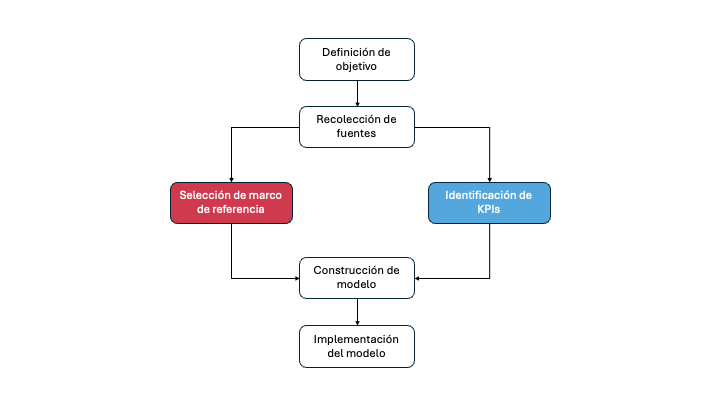
\includegraphics[scale=0.5]{images/4-desarrollo/diagrama-metodologia.png}
    \caption{Metodología utilizada}
    \label{fig:metodologia}
\end{figure}


En la Figura \ref{fig:estrategia} se presenta cual fue, además de la metodología previamente descrita, los componentes y el orden que se tuvieron en cuenta para cada estrategia. Cabe aclarar que no todas las estrategias planteadas contemplaban todos los componentes. Como se verá en la sección \ref{subsec:alternativas-diseno} \nameref{subsec:alternativas-diseno}, los motivos principales por los cuales se descartaron estrategias son por no considerar todos los componentes.  Los ‘Parámetros’ hacen referencia a parámetros que cada estrategia tuvo en cuenta. El primer parámetro, 'Concepto a evaluar', se refiere al componente del ecosistema que se evaluará. Algunos valores válidos pueden incluir ecosistema, servicios ecosistémicos, agua, carbono, especies, entre otros. El 'concepto a evaluar' es el aspecto sobre el cual la empresa está interesada en evaluar sus conocimientos y acciones, y del cual depende e impacta. El parámetro denominado 'Contexto de la empresa' se refiere al sujeto que será evaluado. Esto implica determinar si la estrategia se aplicará a una empresa específica o si se desarrollará para una empresa genérica. El último parámetro, ‘Granularidad empresarial’, se refiere a el nivel de la empresa que será evaluado. Por ejemplo, la granularidad más abstracta hace referencia a toda la empresa, mientras que la granularidad más precisa es un proceso en específico de la empresa. 

\begin{figure}[H]
    \centering
    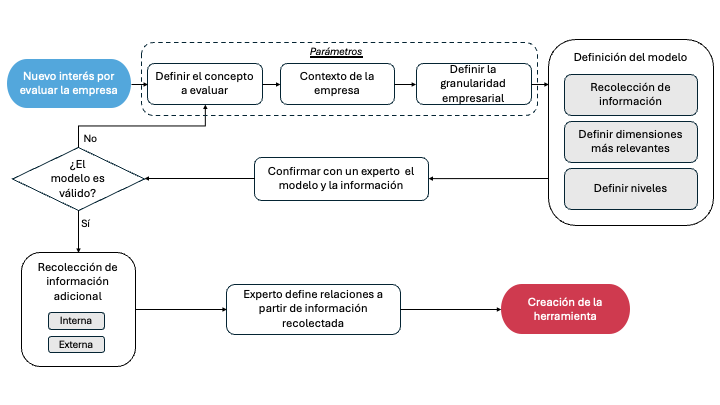
\includegraphics[scale=0.35]{images/4-desarrollo/diagrama-estrategia.png}
    \caption{Estrategia utilizada}
    \label{fig:estrategia}
\end{figure}

El segundo componente de la Figura \ref{fig:estrategia} es ‘Definición del modelo’. De este componente sale el modelo que genera la estrategia. Este es el componte se podría pensar como el más importante de todo el diagrama ya que es el producto “tangible” de la estrategia. Es en la definición del modelo donde comienza y se desarrolla la metodología explicada al principio de esta sección. En el segundo recuadro dentro de ‘Definición del modelo’, ‘Definir dimensiones más relevantes’, es donde se escoge por primera vez los KPIs previamente mencionados.  Por otro lado, ‘Definir niveles de madurez’ es el resultado de aplicar la metodología \textit{benchmarking}, es decir, el resultado de la fase ‘Recolección de información’ . También se podría considerar que el componente denominado 'Definición del modelo' es el resultado de la aplicación individual de la metodología de \textit{benchmarking} a cada subcomponente. El tercer componente del diagrama es la importancia del experto. En la sección \ref{subsec:especificaciones} \nameref{subsec:especificaciones} se habló de cómo era importante que en la herramienta generada de la estrategia no hubiera necesidad de un experto con competencias y conocimiento relacionado al concepto a evaluar (servicio ecosistémico, capital natural, especie, etc.). Sin embargo, en el desarrollo de la estrategia es imperativo la participación del experto. La participación del experto le aporta validez y robustes a la estrategia, ya que, este validará los elementos claves del modelo y la estrategia. Como se puede ver, el experto debe validar el modelo planteado y la información que fue usada y será usada más adelante. Además, el experto es quien se debe responsabilizar de hacer las conexiones entre el negocio y el ecosistema. Como se dijo en secciones anteriores, debido a que no existe una estandarización de relaciones entre elementos de un ecosistema, son los expertos basados en sus opiniones quienes deben determinar esas relaciones. El cuarto componente de este diagrama es la determinación de validez del modelo. A partir de las opiniones y sugerencias del experto, se debe aceptar o no el modelo planteado. En caso en el cual no se acepte el modelo, se debe replantear los tres parámetros a evaluar. Esto se debe a que el modelo puede estar siendo más/menos complejo de lo que en realidad debería ser con respecto al concepto, el contexto y la granularidad empresarial. También, se podría dar el caso que se deban replantear los parámetros debido a la cantidad y calidad de información disponible para la construcción del modelo. Si no hay suficiente información o la calidad de la información es de un grado menor al deseado, las conclusiones y sugerencias que llega el modelo podrán ser sesgas e inconsistentes. El componente ‘Recolección de información adicional’ hace referencia a información que aún falta recolectar sugerida por el experto para continuar con el modelo. La información interna es información relacionada a la empresa o las dimensiones que evalúa la empresa. Esto no significa necesariamente que toda la información interna deba ser de la empresa siendo evaluada. Información interna también puede ser información que un marco de referencia o guía recomienda utilizar para evaluar a una empresa. La información externa, por su parte, hace referencia a la información acerca del concepto a evaluar (ecosistema, capital natural, servicio ecosistémico, etc.) que el experto necesita para poder determinar las relaciones. Por último, la ‘Creación de la herramienta’ es el paso final de este diagrama. Esta herramienta tendrá toda la información creada y obtenida en los anteriores pasos. Por lo tanto, la herramienta será la que permita a la empresa saber su nivel con respecto al concepto que se está evaluando. 


\subsection{Recolección de información} \label{subsec:recoleccion-informacion}
La metodología de \textit{benchmarking} requiere utilizar un amplio número de fuentes de información. En el caso de este proyecto, las fuentes de información fueron utilizadas para determinar las dimensiones (\acrshort{kpis}), los niveles de madurez, los indicadores, las preguntas por dimensión que evalúan a la empresa, conceptos de evaluación, entre otras. A continuación se hará una descripción de las siete (7) fuentes de información más importantes. Existen otras fuentes de información que fueron utilizadas con un menor grado de importancia, por lo tanto, no serán explicadas a detalle. Estas fuentes de información fueron: \parencite{alliance-for-water-stewardship-2019}, \parencite{gri-2022}, \parencite{iso-1999}, \parencite{pacific-institute-2014}, \parencite{world-business-council-for-sustainable-development-2011}, \parencite{world-resources-institute-2008}, \parencite{world-wildlife-fund-2021}, \parencite{taskforce-on-nature-related-financial-disclosures-2023} y \parencite{climate-disclosure-standards-board-2022}

\subsubsection{\textit{Capital Natural Protocol}}
El \textit{Capital Natural Protocol} es un marco de referencia creado por Capital Colation que está diseñado para crear información valiosa para la toma de decisiones por parte de la altas directivas. El protocolo pretende apoyar mejores decisiones incluyendo cómo interactuamos con la naturaleza, o más específicamente con el capital natural, en la toma de decisiones \textit{\parencite{capitals-coalition-2021}}. Este documento tiene un marco de referencia divido en 4 etapas (Tabla \ref{tab:cnp-etapas}) , cada una con series de preguntas y objetivos que se deben responder y cumplir, respectivamente, para pasar a la siguiente etapa. 

\begin{table}[h!]
    \centering
    \begin{tabular}{p{3.5cm} | p{8cm} | p{3cm}}
        \centering\textbf{Etapa} & \centering\textbf{Definición}  & \textbf{Pregunta} \\
        \hline\hline
        \textit{Frame} & Identificar qué impactos de capital natural y/o dependencias son relevantes para el negocio.  & ¿Por qué?\\
        \hline
        \textit{Scope} & Establece lo que tendrá que considerar para establecer el objetivo específico para su evaluación del capital natural. & ¿Qué? \\
        \hline
        \textit{Measure and Value} & Cómo se pueden medir los impactos y las dependencias y cuál es el valor de los impactos y dependencias del capital natural. & ¿Cómo? \\
        \hline
        \textit{Apply} & Ayuda a interpretar, aplicar y actuar sobre los resultados del negocio.  & ¿Qué sigue? \\
        \hline
    \end{tabular}
    \caption{Etapas del \textit{Capital Natural Protocol} \parencite{capitals-coalition-2021}}
    \label{tab:cnp-etapas}
\end{table}

Para el desarrollo de este proyecto solo se tuvieron en cuenta las primeras etapas, ya que la cuarta etapa menciona futuros cambios y acciones, lo cuales no fueron contemplados ya que están asociados a las oportunidades y riesgos. El protocolo se basa en los siguientes cuatro (4) principios: relevancia, la cual busca que la empresa este considerando los problemas o circunstancias realmente más importantes; rigor, la información y los datos utilizados deben venir de perspectivas científicas o económicas; replicabilidad, todos los supuestos, datos y métodos utilizados son transparentes, documentados y repetibles; y, por último, consistencia, los datos y métodos utilizados durante el uso del marco de referencia son compatibles entre ellos, además de depender de los objetivos y expectativas de la aplicación del marco de referencia \parencite{capitals-coalition-2021}.



\subsubsection{ISO 14001 e ISO 14004}
Las normas de la Organización Internacional de Normalización (ISO) son utilizadas como marcos de referencias que ayudan a diferentes organizamos en diferentes contextos a lograr algún objetivo basándose en una estructura y estándares específicos. La norma ISO 14001 denominada “Sistemas de Gestión Ambiental – Requisitos con orientación para su uso” \parencite{iso-2015} fue la fuente principal para determinar las dimensiones (KPIs) que serían evaluadas para determinar el nivel de la empresa. En la sección \ref{sec:implementacion}. \nameref{sec:implementacion} se entra en mayor detalle de cómo se utilizó cada una de las dimensiones. Sin embargo, debido al objetivo de la ISO 14001, se considera que cada sección de la guía contempla las dimensiones clave que deben tenerse en cuenta al evaluar una empresa. El objetivo, según la guía \textcite{iso-2015}, es

\hfill
\par
\leftskip=0.35in \rightskip=0.35in
Esta Norma Internacional especifica los requisitos de un sistema de gestión ambiental para organizaciones que buscan establecer, implementar, mantener y mejorar continuamente un marco de referencia con el fin de gestionar sus responsabilidades ambientales de una forma que contribuya al “pilar ambiental” de la sostenibilidad.

\hfill
\par
\leftskip=0in \rightskip=0in
Por otro lado, la norma  ISO 14004 denominada “Sistemas de gestión ambiental – Directrices generales sobre principios, sistemas y técnicas de apoyo” \parencite{iso-2004} fue utilizada principalmente para evaluar la dimensión de Soporte. Es decir, la norma ISO 14004 fue utilizada para evaluar la empresa en sector de capital humano, específicamente, en los recursos, educación y comunicación brindada a los trabajadores dentro de la empresa. La razón principal de haber utilizado esta guía para evaluar dicha dimensión se debe a la justificación que presenta la misma norma. 

\hfill
\par
\leftskip=0.35in \rightskip=0.35in
Facilitar informaci\'on apropiada a los empleados de una organizaci\'on sirve para motivarlos y para fomentar la aceptaci\'on de los esfuerzos de la organizaci\'on para mejorar su desempe\~no ambiental. Esto puede ayudar a los empleados a cumplir sus responsabilidades y a la organizaci\'on a cumplir sus objetivos y metas ambientales. La organizaci\'on deber\'ia contar con un proceso para fomentar la retroalimentaci\'on y el compromiso de todos los niveles de la organizaci\'on, y recibir y responder las sugerencias e inquietudes de los empleados \parencite{iso-2004}. 

\hfill
\par
\leftskip=0in \rightskip=0in

El extracto anterior se considera que está alineado con las importancias ya mencionadas en la sección \ref{subsec:identificacion-problema-importancia}. \nameref{subsec:identificacion-problema-importancia}. La estrategia que se busca implementar dentro de este documento considera que la participación de todos los trabajadores involucrados dentro de la empresa debe ser actores activos. La mejora, el cambio y el progreso hacia un mejor nivel debe estar acompañado por un alineamiento unánime de todos los actores dentro de la empresa. 

\subsubsection{GRI 303: Agua y efluentes 2018}

La “GRI 303: Agua y efluentes 2018 incluye contenidos para que las organizaciones presenten información acerca de sus impactos relacionados con el agua y la manera en que gestionan estos impactos” \parencite{gri-2019}. La guía GRI 303 hace parte de los estándares GRI, los cuales, tienen como objetivo informar de la mejor manera a una empresa, ente gubernamental o grupo de personas específicas acerca de un impacto económico, ambiental o social.  La guía GRI 303 fue utilizada debido a que presenta información valiosa que una empresa debería tener en cuenta cuando trata con agua. El documento presenta tres secciones que solicitan a una empresa, que desee seguir el estándar, documentar y medir. La extracción del agua, el vertido del agua y el consumo del agua son tres componentes que una empresa debe medir y documentar para determinar el impacto sobre ecosistemas relacionados con el agua. Estos tres componentes fueron tenidos en cuenta a la hora de desarrollar la herramienta, ya que en la etapa de indicadores, se evalúan estos tres componentes.


\subsubsection{SASB}
Los estándares SASB tienen por objeto ayudar a las entidades a revelar información sobre los riesgos y oportunidades relacionados con la sostenibilidad que razonablemente podrían afectar a los flujos de efectivo de la entidad, su acceso a la financiación o el coste del capital a corto, medio o largo plazo \parencite{sasb-standards-2023}. Debido al reconocimiento global de este estándar, a la facilidad de uso de su página web y al consejo del experto, se decidió utilizar la clasificación de sectores e industrias proporcionada por dicho estándar. Este estándar también presenta un amplio repertorio de indicadores relacionados a diversos capitales naturales que fueron utilizados para relacionar a la empresa con los ecosistemas.  


\subsubsection{Manual de Estrategias para la Naturaleza}
Según \textcite{its-now-for-nature-2023} en su  “Manual de Estrategias para la Naturaleza”,

\hfill
\par
\leftskip=0.35in \rightskip=0.35in
El objetivo del Manual de Estrategias para la Naturaleza es apoyar a todas las empresas, ya sean corporaciones o instituciones financieras, en el desarrollo de una estrategia para la naturaleza que les permita contribuir significativamente a un mundo positivo para la naturaleza.

\hfill
\par
\leftskip=0in \rightskip=0in
El manual utilizada la metodología Evaluar, Comprometerse, Transformar y Divulgar (ACT-D) \parencite{its-now-for-nature-2023}, la cual guía a las empresas a través de diferentes herramientas y les ayuda, también, a fijar objetivos relacionados a disminuir el impacto en la naturaleza. Este manual es de gran importancia para el desarrollo de este documento y la generación de preguntas en la implementación de la herramienta. El Manual de Estrategias para la Naturaleza, fue utilizado como corroboración y revisión de preguntas en el paso de Cuestionario en el despliegue de la aplicación web (\ref{subsec:implementacion-desarrollo-herramienta}. \nameref{subsec:implementacion-desarrollo-herramienta}). 


\subsubsection{\textit{CDP Water Security 2023 Questionnaire}}

Esta fuente de información fue la fuente principal para el desarrollo del cuestionario de la aplicación web. El cuestionario de agua ayuda a las empresas a impulsar mejoras en la gestión del agua y permite la comparación con las prácticas líderes \parencite{disclosure-insight-action-2023}. Aunque en el documento se establece que el cuestionario está orientado a riesgos y oportunidades, muchas de las preguntas incluidas están relacionadas con las dependencias e impactos. El cuestionario está dividido en diez (10) secciones diferentes, las cuales buscan evaluar cada dimensión de una empresa para determinar los riesgos y oportunidades posibles. Estas diez (10) dimensiones no fueron escogidas sobre las proporcionadas por la ISO 14001, ya que las dimensiones del \textcite{disclosure-insight-action-2023} están orientadas a riesgos y oportunidades en lugar de dependencias e impactos. Además, no todas las dimensiones de este cuestionario se consideran relevantes, mientras que todas las dimensiones de la ISO 14001 sí se consideran vitales para la evaluación de la empresa. Según \textcite{disclosure-insight-action-2023}, existen 85 preguntas sin incluir preguntas específicas por sector o de cadena de suministro. Esto se debe a que el camino que toma cada empresa será diferente dependiendo no solo de su sector, sino respuestas en diferentes dimensiones que desencadenan preguntas específicas.

\subsection{Alternativas de diseño} \label{subsec:alternativas-diseno}
La Figura \ref{fig:estrategia} muestra cuál fue la manera genérica que se evaluó cada estrategia considerada. En esta sección se explicará las dos estrategias que se plantearon que no fueron escogidas. Se explicará el objetivo principal de la estrategia, los parámetros considerados, el modelo desarrollado y las razones por las cuales no fue escogida. 

\subsubsection{Estrategia: Primer acercamiento}
La estrategia 'Primer acercamiento' fue la primera estrategia que fue planteada y analizada para este proyecto. Como se puede ver en la Figura \ref{fig:primer-acercamiento} la estrategia incluye cuatro pasos principales, no incluye un modelo explícitamente y de los parámetros solo es tomado en cuenta el contexto de la organización. El objetivo principal de esta estrategia era proporcionarle información extra a la empresa según el estado actual de la misma. En el primer paso, y único parámetro tenido en cuenta, se buscaba comprender el contexto de la organización. En este paso se busca obtener la información geográfica de la empresa, su sector e industria, y por cada servicio ecosistémico que la empresa usara sus dependencias, impactos, riesgos y oportunidades. En este paso ya se pueden ver varios inconvenientes. El primero es la falta de información adicional que no se le pedía a la empresa. Al solo pedirle la ubicación geográfica o su sector e industria se estaban incurriendo en los mismos problemas que las herramientas \nameref{subsubsec:encore} y \nameref{subsubsec:wwf-water-risk-filter}. Adicionalmente, se estaba haciendo un supuesto bastante flexible y errónea en cual consistía que las empresas sabían desde un principio todos los \acrshort{ssee} de los cuales dependerían, impactaban, tenían riesgos y oportunidades. Entonces, bajo este supuesto, el objetivo de esta estrategia se perdía ya que, si la empresa no sabía nada, se le tendría que mostrar toda la información disponible en la herramienta. El problema de lo anterior es que si se le muestra toda la información disponible cuando la empresa desde un principio no tiene información, es muy probable que esta no vaya a saber cómo utilizarla, aprovecharla y aplicarla.

\begin{figure}[h!]
    \centering
    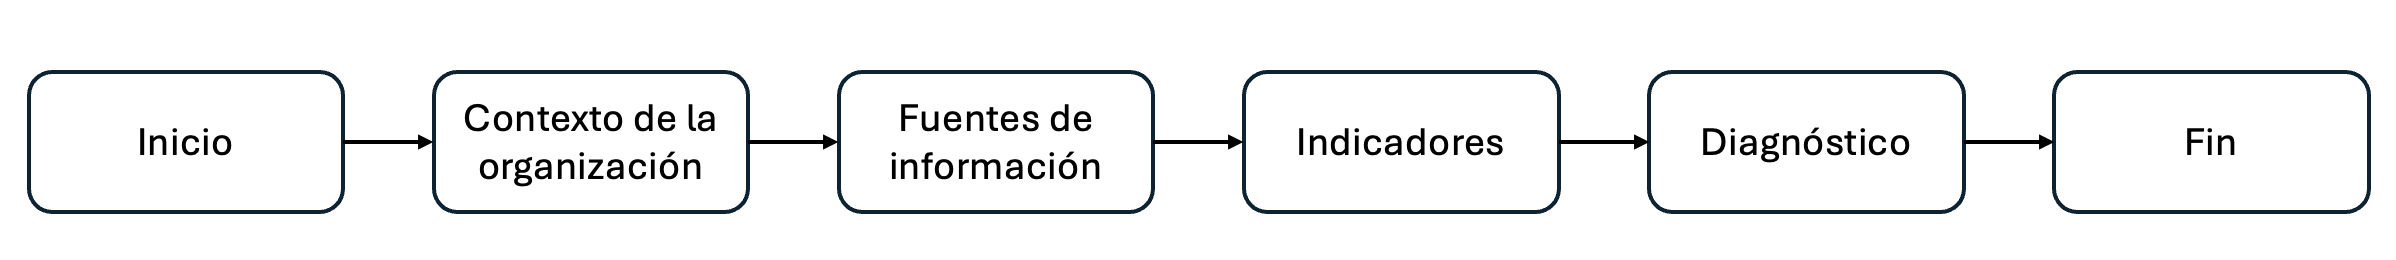
\includegraphics[scale=0.35]{images/4-desarrollo/estrategia-primer-acercamiento.png}
    \caption{Primer acercamiento}
    \label{fig:primer-acercamiento}
\end{figure}

El siguiente paso en la Figura \ref{fig:primer-acercamiento} denominado ‘Fuentes de información’ consistía en obtener las fuentes de información que la empresa utilizaba. Este paso sufría el mismo problema que el paso anterior. Cuando la empresa no tenía información este paso no se podría aplicar, es decir, el 25\% de la estrategia sería inutilizable. Cuando la empresa si tenía información, la intención de este paso era analizar y evaluar dicha información. Evaluar su temporalidad, rigurosidad, confiabilidad, utilidad, granularidad, comparabilidad, etc. A partir de estas dimensiones, se le mostraría a la empresa su nivel con respecto a la información que utiliza. 

El propósito del tercer paso, ‘Indicadores’, dependía directamente de los anteriores dos pasos. La intención era mostrarle a la empresa los indicadores que existían según la información que esta tenía. Entonces, si la empresa no tenía información, no se podía evaluar y adicionalmente, no se le podía mostrar indicadores. Por lo tanto, se estaría perdiendo 50\% de la estrategia. Se podría pensar en el caso que la empresa no tenga nada de información mostrarle toda la disponible más todos los indicadores disponibles, pero se estaría cayendo en una trampa. Si se le muestra toda la información y sus indicadores respectivos sin ninguna asistencia o guía, la empresa no sabría que hacer con ella. Este paso, por otro lado, no contemplaba el hecho que las empresas podían estar midiendo indicadores adicionales a los disponibles. Esto perjudicaba a la empresa ya que no le permitía analizar sus indicadores actuales. 

Finalmente, en el último paso, ‘Diagnóstico’, se busca mostrar un nivel de madurez con respecto a los tres anteriores pasos. Es decir, a partir de la información obtenida en el contexto de la organización y la evaluación de lo información que dispone la empresa, se determinaba un nivel de madurez. En el momento que se estaba desarrollando esta estrategia nunca se llegó a pensar en sus KPIs, lo cual, es otro indicio porque esta estrategia no fue aplicada. En conclusión, esta estrategia no fue aplicada debido a la alta dependencia entre cada etapa, la falta de rigurosidad y la generalización de las empresas. Además, no mostraba indicios de concienciar a las empresas para realizar cambios hacia el cuidado y la sostenibilidad de los ecosistemas. Finalmente, la estrategia no contemplaba la ayuda u opinión de expertos, y como ya se explicó en secciones anteriores, a opinión y conocimientos de estos es muy importante en el contexto de los ecosistemas y sus componentes. 

\subsubsection{Matriz de dimensiones} \label{subsubsec:matriz-dimensiones}
La segunda estrategia que fue tomada en cuenta se llamó Matriz de dimensiones. En la Figura \ref{fig:estrategia-matriz-dimensiones} se puede observar la estrategia que se llevó a cabo. Esta estrategia busca determinar el nivel de una empresa contemplando todos los \acrshort{ssee} de la cual esta dependía e impactaba. A pesar de que esta estrategia estaba dirigida a una empresa genérica, la granularidad empresarial era un proceso específico de la empresa. Entonces, el objetivo de esta estrategia era determinar el nivel de madurez de una empresa según las dependencias e impactos que tenía sobre todos los \acrshort{ssee} que utilizase en un proceso en específico.

\begin{figure}[h!]
    \centering
    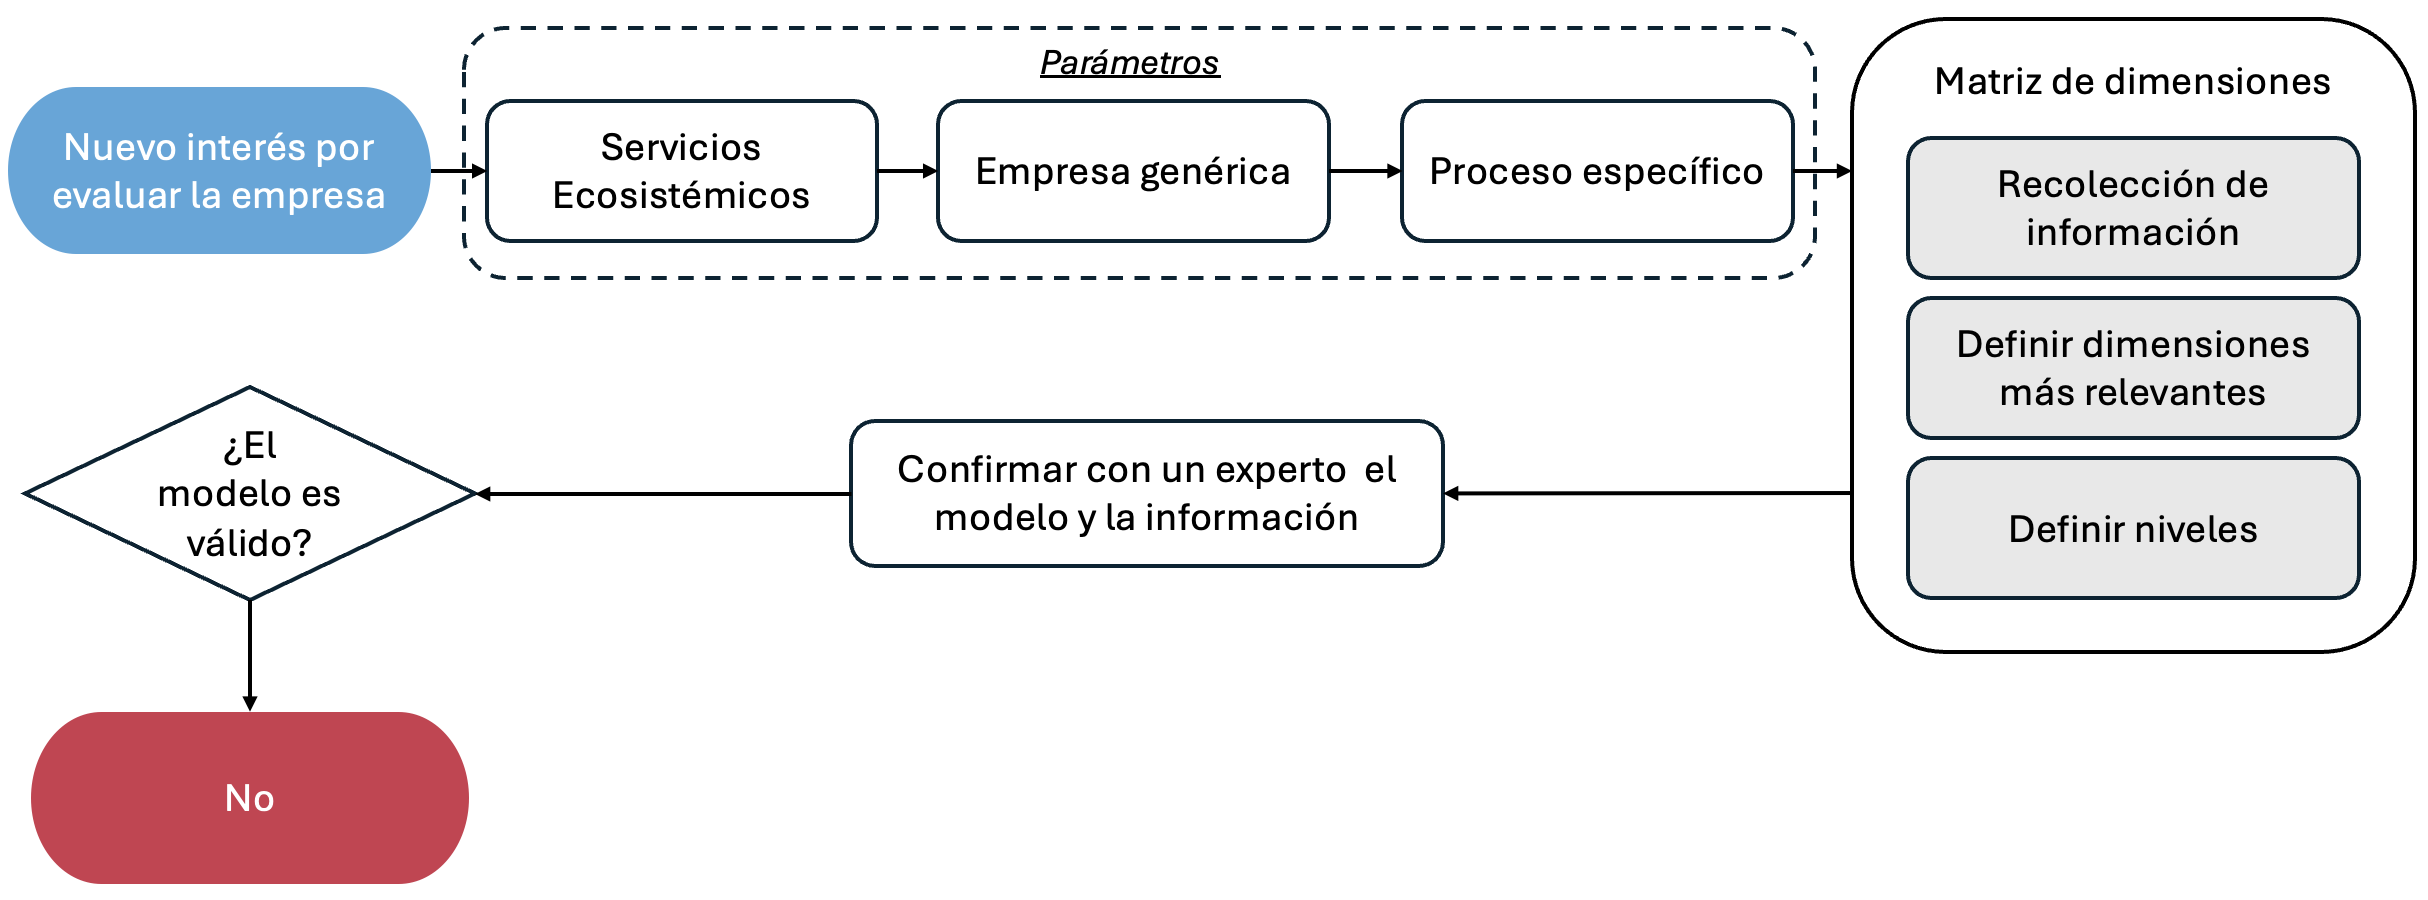
\includegraphics[scale=0.35]{images/4-desarrollo/estrategia-matriz-dimensiones.png}
    \caption{Diagrama de la estrategia Matriz de dimensiones}
    \label{fig:estrategia-matriz-dimensiones}
\end{figure}

En la Figura \ref{fig:proceso-matriz-dimensiones} se muestra el paso que se debía hacer antes de implementar la estrategia. En este paso se determinaba cuál proceso de la empresa se evaluaría. Primero, se escogían todos los procesos candidatos de la empresa. Según los objetivos del negocio, la factibilidad de cambio, los dolores que generaban no tener el proceso evaluado, las necesidades que surgían del proceso y las oportunidades que tiene el proceso se graficaba el proceso. Teniendo en cuentas todas las anteriores variables, se determinaba el impacto y la factibilidad, es decir, cuál es el impacto tanto a nivel empresarial como ecosistémico de cambiar el proceso versus cuál es la factibilidad de ese cambio. El proceso que tuviera el mayor impacto y la mayor factibilidad era el escogido para ser evaluado.  

\begin{figure}[H]
    \centering
    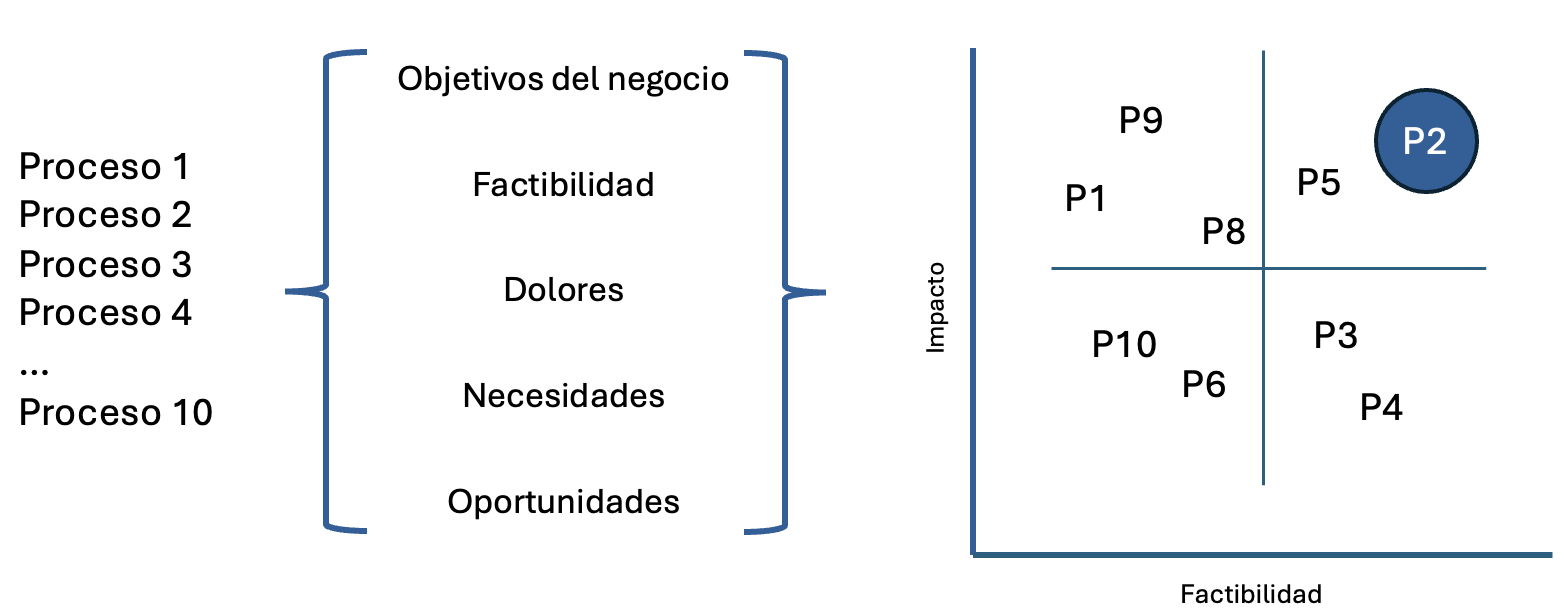
\includegraphics[scale=0.45]{images/4-desarrollo/proceso-matriz-dimensiones.png}
    \caption{Etapas para escoger el proceso en la estrategia Matriz de dimensiones}
    \label{fig:proceso-matriz-dimensiones}
\end{figure}

Cuando ya se hubiera escogido el proceso se procedía a evaluarlo. Esta evaluación se hacía a partir de modelo escogido en esta estrategia denominado Matriz de dimensiones \ref{fig:matriz-dimensiones}. Este modelo buscaba evaluar el proceso en cada una de las dimensiones que se ven en el diagrama. Por cada dimensión se le otorgaba un nivel, siendo uno (1) el peor nivel y cinco (5) el mejor. Luego de tener el nivel para cada dimensión, se determinaba el nivel general del proceso. En la Tabla \ref{tab:matriz-dimensiones} se puede ver la descripción de cada dimensión que evaluaba al proceso.

\begin{figure}[H]
    \centering
    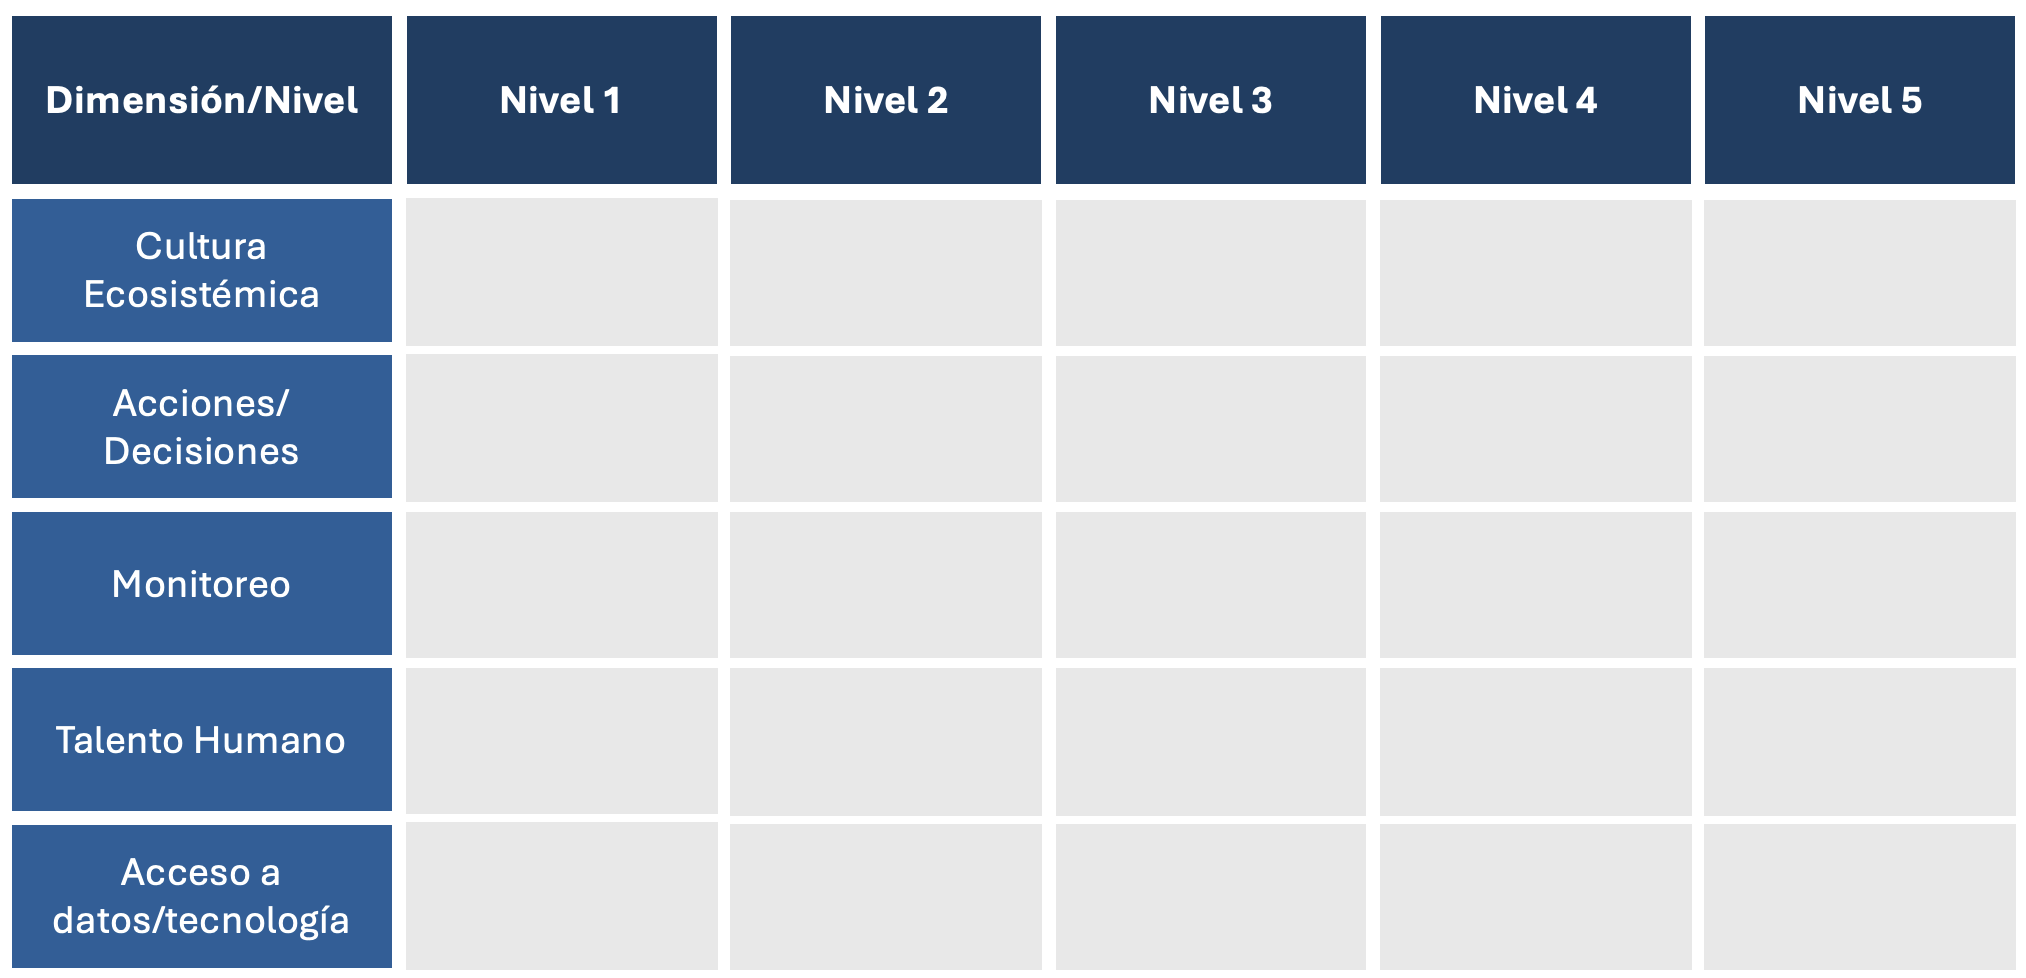
\includegraphics[scale=0.4]{images/4-desarrollo/matriz-dimensiones.png}
    \caption{Matriz de dimensiones}
    \label{fig:matriz-dimensiones}
\end{figure}


\begin{table}[H]
    \centering
    \begin{tabular}{p{5cm} | p{10cm}}
        \textbf{Dimensión} & \textbf{Descripción} \\
        \hline\hline
        Cultura Ecosistémica & Conocimiento y comprensión que tiene una empresa sobre su relación con los ecosistemas, incluyendo sus dependencias, impactos y el contexto ecosistémico de sus procesos.\\
        \hline
        Acciones/ Decisiones & El concepto de SSEE hace parte de la toma de decisiones y acciones hechas en el proceso.\\
        \hline
        Monitoreo & Seguimiento regular y evaluaciones periódicas de la relación entre un proceso y el ecosistema, incluyendo sus costos en términos de dinero, tiempo y mano de obra.\\
        \hline
        Talento Humano & Calidad del conjunto de personas, tanto internas como externas, involucradas en un proceso. \\
        \hline
        Acceso a datos/tecnología & Disponibilidad, facilidad de obtención y uso de datos y tecnologías para la recolección y análisis de información en un proceso.\\
        \hline
    \end{tabular}
    \caption{Explicación de dimensiones en Matriz de dimensiones}
    \label{tab:matriz-dimensiones}
\end{table}

El principal problema de la estrategia Matriz de dimensiones era la falta de información rigurosa o estandarizada para responder la pregunta “¿Qué significa ser nivel X para la dimensión Y?”.  Debido que calificar al proceso dependía del nivel por dimensión, la respuesta a la anterior pregunta debía tener un soporte, formalidad, estandarización y rigurosidad que actualmente no existe. Como bien se ha dicho en este documento, la opinión de los expertos es vital para cualquier estrategia debido a la falta de estandarización en el campo. Sin embargo, basar todo el modelo en la opinión de expertos es ir al extremo radical, el cual es un error. Cuando determinar qué significa ser nivel X en la dimensión Y para cada nivel por cada dimensión basándose en la opinión del experto, es más que probable que el modelo vaya a ser sesgado e inconsistente. No solo por la falta de información, sino porque no hay unanimidad en el contexto de los ecosistemas para aceptar 25 calificaciones (5 dimensiones x 5 niveles).

El segundo problema, algo relacionado con el primero, era la falta de formalidad que tenía la escogencia de las dimensiones. Las dimensiones presentadas en la matriz no vienen de ningún marco de referencia, manual, guía o estándar ya existente. Esto genera que exista posibles confusiones ya que a pesar de que se pueda definir la dimensión, no existe una fuente confiable que expanda sobre esta. Esto quiere decir, que el modelo no solo puede llegar a confundir, sino que también es necesario hacer una extensión por cada dimensión escogida. Explicarla detalladamente, justificar por qué no se escogieron más y por qué es suficiente solo estas dimensiones son las preguntas que se deberían responder.  El ejercicio anterior se podría hacer, el inconveniente es que no existe un respaldo oficial sobre este. En cambio, todos los componentes de la estrategia escogida en este documento fueron basados en marcos de referencia, manuales, guías o estándares ya existente. Esto le da validez, formalidad y soporte a la estrategia, algo que no es posible para la estrategia Matriz de dimensiones.


\section{Implementación} \label{sec:implementacion}
Aplicando la metodología \textit{benchmarking}, planteando posibles estrategias bajo parámetros diferentes y la revisión continua de expertos se llegó a la estrategia solución Negocio-Agua. El diagrama de flujo y los componentes de esta estrategia se puede ver en la Figura \ref{fig:estrategia-negocio-agua}. La estrategia solución usa al agua como concepto a evaluar, se hace sobre una empresa genérica y se contempla toda la empresa.  El agua como capital natural fue escogido para evaluar ya que es uno de los capitales natural más prácticos y sencillos para evaluar al tiempo que es uno de los capitales naturales con más información disponible. Es importante que la primera estrategia que implementará la empresa es con un elemento sencillo de evaluar. No solo facilita el entendimiento de la estrategia y la herramienta, sino que posiblemente puede motivar a la empresa a evaluar otros capitales naturales. Adicionalmente, el agua como capital natural, como bien se ha demostrado su importancia a través de este documento, tiene bastante información relacionada a todas las metas, iniciativas y objetivos que se buscan cumplir en el corto y largo plazo.  Debido que todas las industrias de todos los sectores utilizan el agua en algún momento de su cadena de producción, operaciones o ventas, se considera que hacer esta estrategia, y por su consecuencia la herramienta, de manera genérica tendrá mayor utilidad y prospecto. El agua al ser un recurso compartido por todos los seres vivos en el mundo, debe ser un trabajo de todos mejorar las condiciones actuales y futuras. Al implementar esta estrategia de manera genérica, se busca que más empresas pueda utilizar esta herramienta para que así, como país, se puedan mejorar las condiciones del agua, al tiempo que se cumplen con metas y objetivos internacionales. Finalmente, se considera a toda la empresa como agente a evaluar ya que el uso del agua dentro de una empresa esta interconectada entre diferentes líneas de negocio, procesos y recursos. Se considera que una evaluación sobre un único proceso, como en el caso de la estrategia Matriz de dimensiones, no sería lo más optimo ya que puede que se escoja un proceso con poca utilización de agua y genere resultados falsos y no producentes para la empresa. 

\begin{figure}[H]
    \centering
    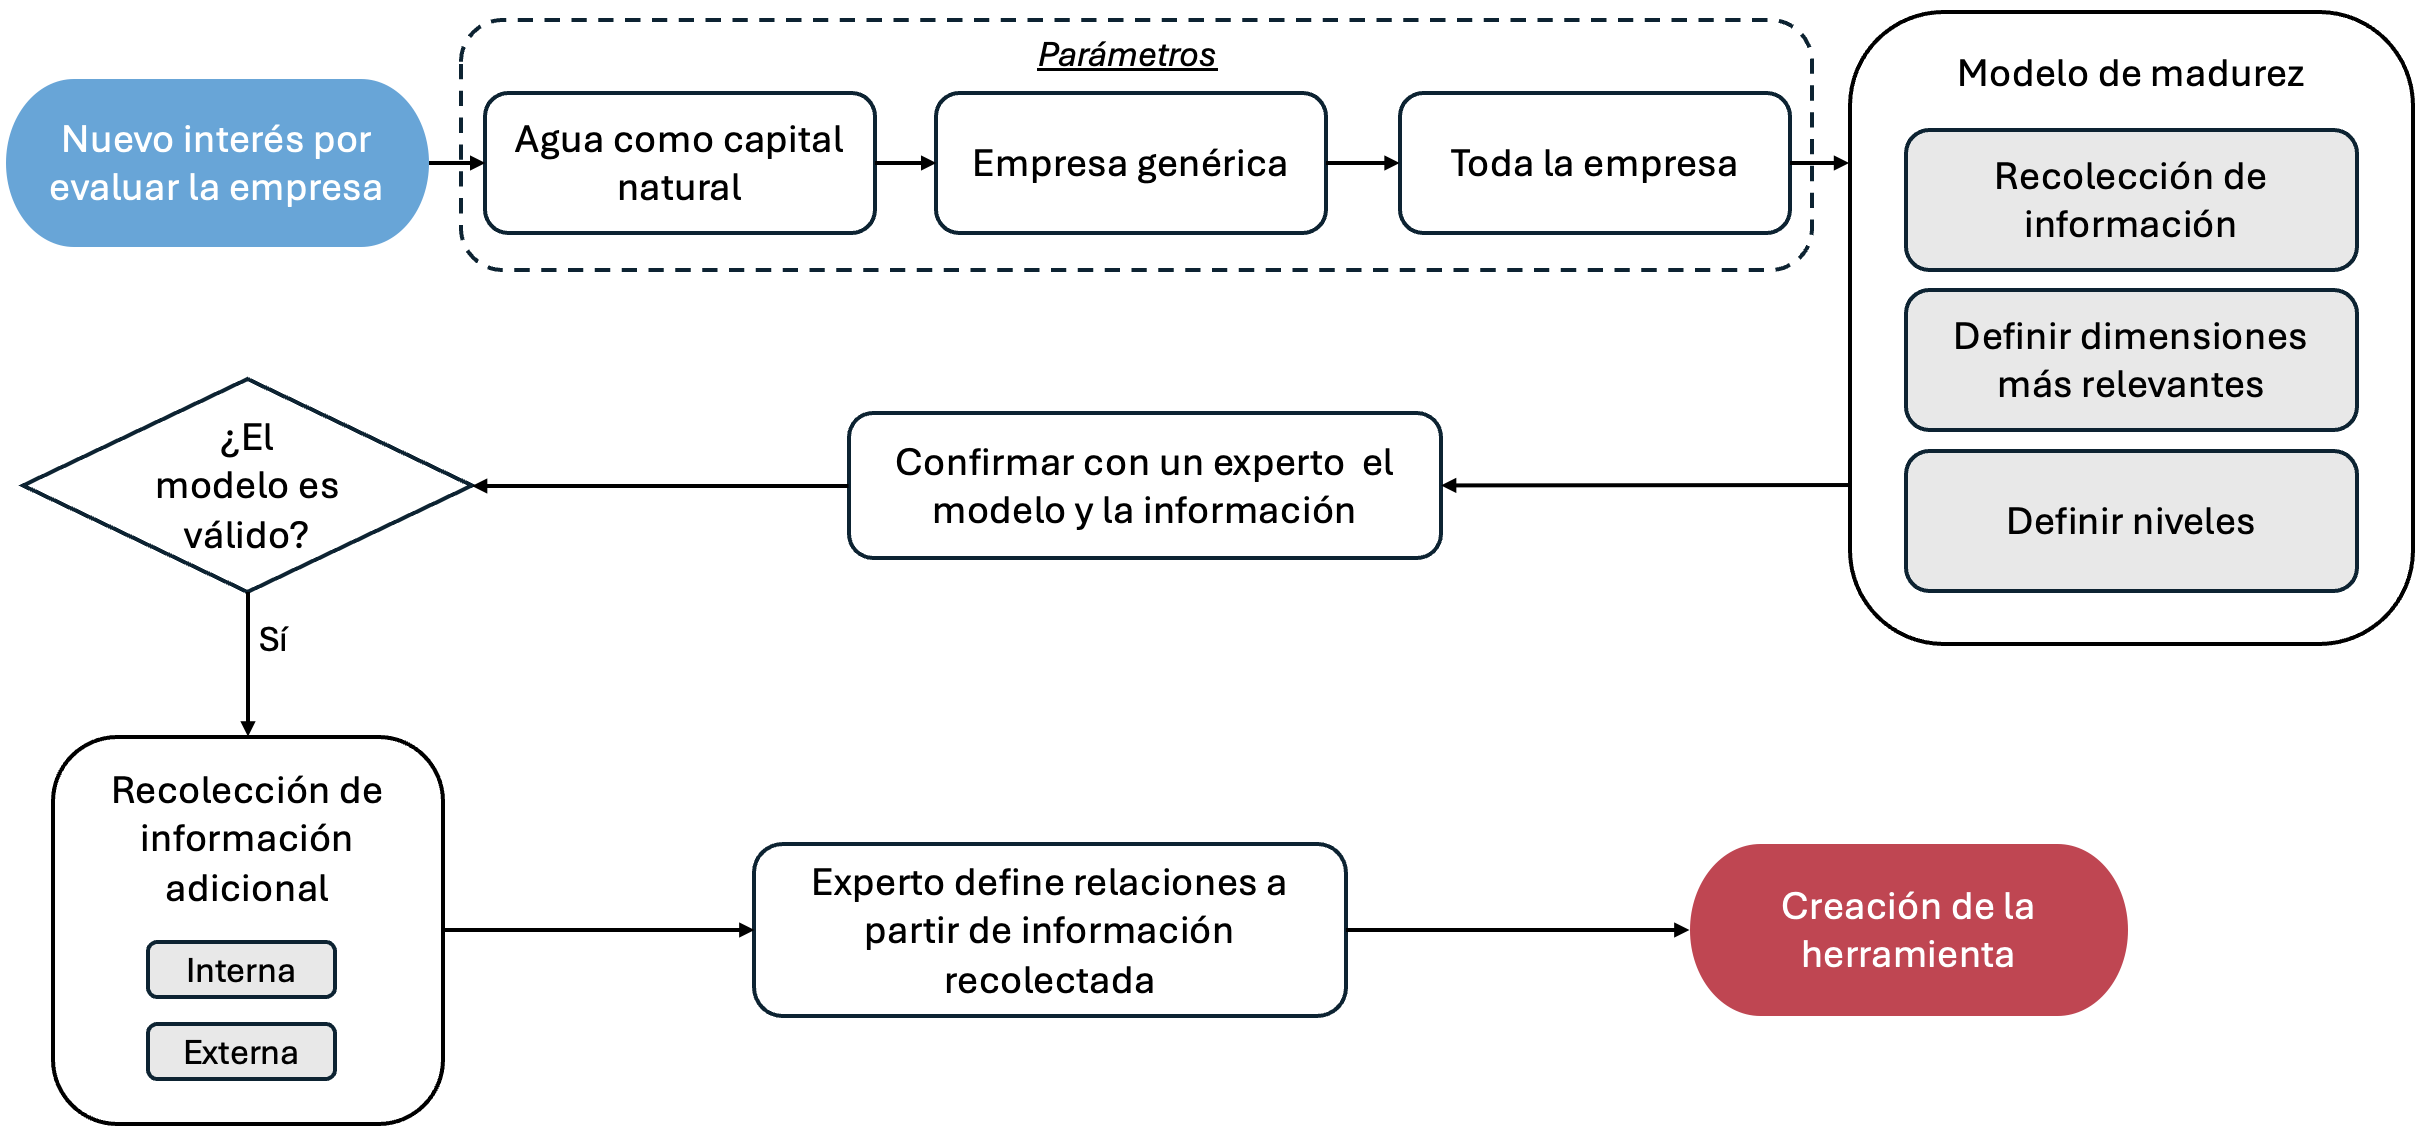
\includegraphics[scale=0.25]{images/5-implementacion/estrategia-negocio-agua.png}
    \caption{Flujo de la estrategia Negocio-Agua}
    \label{fig:estrategia-negocio-agua}
\end{figure}

Luego de haber definido los parámetros que serán evaluados en esta estrategia, se procede a crear el modelo de madurez que evalué a la empresa. El modelo de madurez fue realizado utilizando la metodología descrita en la sección \ref{sec:desarrollo-diseno}. \nameref{sec:desarrollo-diseno} , utilizando las fuentes de información descritas en la sección \ref{subsec:recoleccion-informacion}. \nameref{subsec:recoleccion-informacion}. Este modelo está compuesto por siete dimensiones que evalúan a la empresa y cuatro niveles posibles de clasificación.  En la siguiente sección se describirá en mayor detalle el modelo de madurez y sus componentes.

La información adicional que se requirió para completar el modelo y la estrategia fue principalmente información externa. Como dicho en la sección \ref{sec:desarrollo-diseno}. \nameref{sec:desarrollo-diseno}  la información externa hace referencia a la información acerca del concepto a evaluar, en este caso el agua como capital natural, que el experto necesita para poder determinar las relaciones. En especial, la información adicional recolectada estuvo relacionada a indicadores de agua, servicios, funciones y gestiones ecosistémicas relacionadas al agua. Adicionalmente, para mayor robustez del modelo, la experta M.A. Parra sugirió implementar la metodología \textit{Analytic Hierarchy Process} la cual será explicada en la siguiente sección. Finalmente, luego de tener toda la información, la validación del modelo, las relaciones entre el negocio y el agua establecidas se puedo hacer la creación de la herramienta. La implementación de la herramienta fue hecha a través de una aplicación web. El objetivo de la herramienta es desarrollar e implementar el modelo generado por la estrategia para determinar el nivel de madurez de la empresa, al mismo tiempo que se visualiza su relación con el agua a partir de la información proporcionada por la misma empresa. Más detalles e imágenes de la aplicación web serán mostrados en la sección \ref{subsec:implementacion-desarrollo-herramienta}. \nameref{subsec:implementacion-desarrollo-herramienta}.

\subsection{Descripción de la implementación} \label{subsec:descripcion-implementacion}

En esta sección se explicará cada componente de la estrategia en detalle. Primero, se explicará el modelo de madurez generado por la estrategia y todos sus componentes. Luego, se procederá a explicar la metodología \textit{Analytic Hierarchy Process}, la cual fue implementada para darle mayor robustez al modelo. Por último, se mostrarán las relaciones entre el negocio y el agua que se generaron y la manera en que fueron establecidas.

\subsubsection{Modelo de madurez}
Un modelo de madurez según \textcite{poppelbu-2011} en su artículo \textit{What Makes a Useful Maturity Model? A Framework of General Design Principles for Maturity Models and Its Demonstration in Business Process Management} es:

\hfill
\par
\leftskip=0.35in \rightskip=0.35in
[…] un marco estructurado que describe las etapas de evolución y mejora en un área de interés particular, como procesos, capacidades o entidades. Típicamente consiste en una serie de niveles o etapas que representan niveles crecientes de madurez o sofisticación. Los modelos de madurez se utilizan para evaluar el estado actual de una organización o sistema, identificar áreas de mejora y proporcionar una hoja de ruta para avanzar hacia niveles más altos de madurez.

\hfill
\par
\leftskip=0in \rightskip=0in

En el caso de este documento, el modelo de madurez (Figura \ref{fig:modelo-madurez}) originado de la estrategia Negocio-Agua, determina el nivel de madurez de una empresa en cuanto a sus conocimientos y acciones sobre las dependencias e impactos que tiene sobre el agua como capital natural. Los cuatro niveles que componen este modelo de madurez están basados en los niveles del proyecto \textit{Valuing Water Finance Initiative Benchmark} \parencite{ceres-2023B}.

\begin{figure}[H]
    \centering
    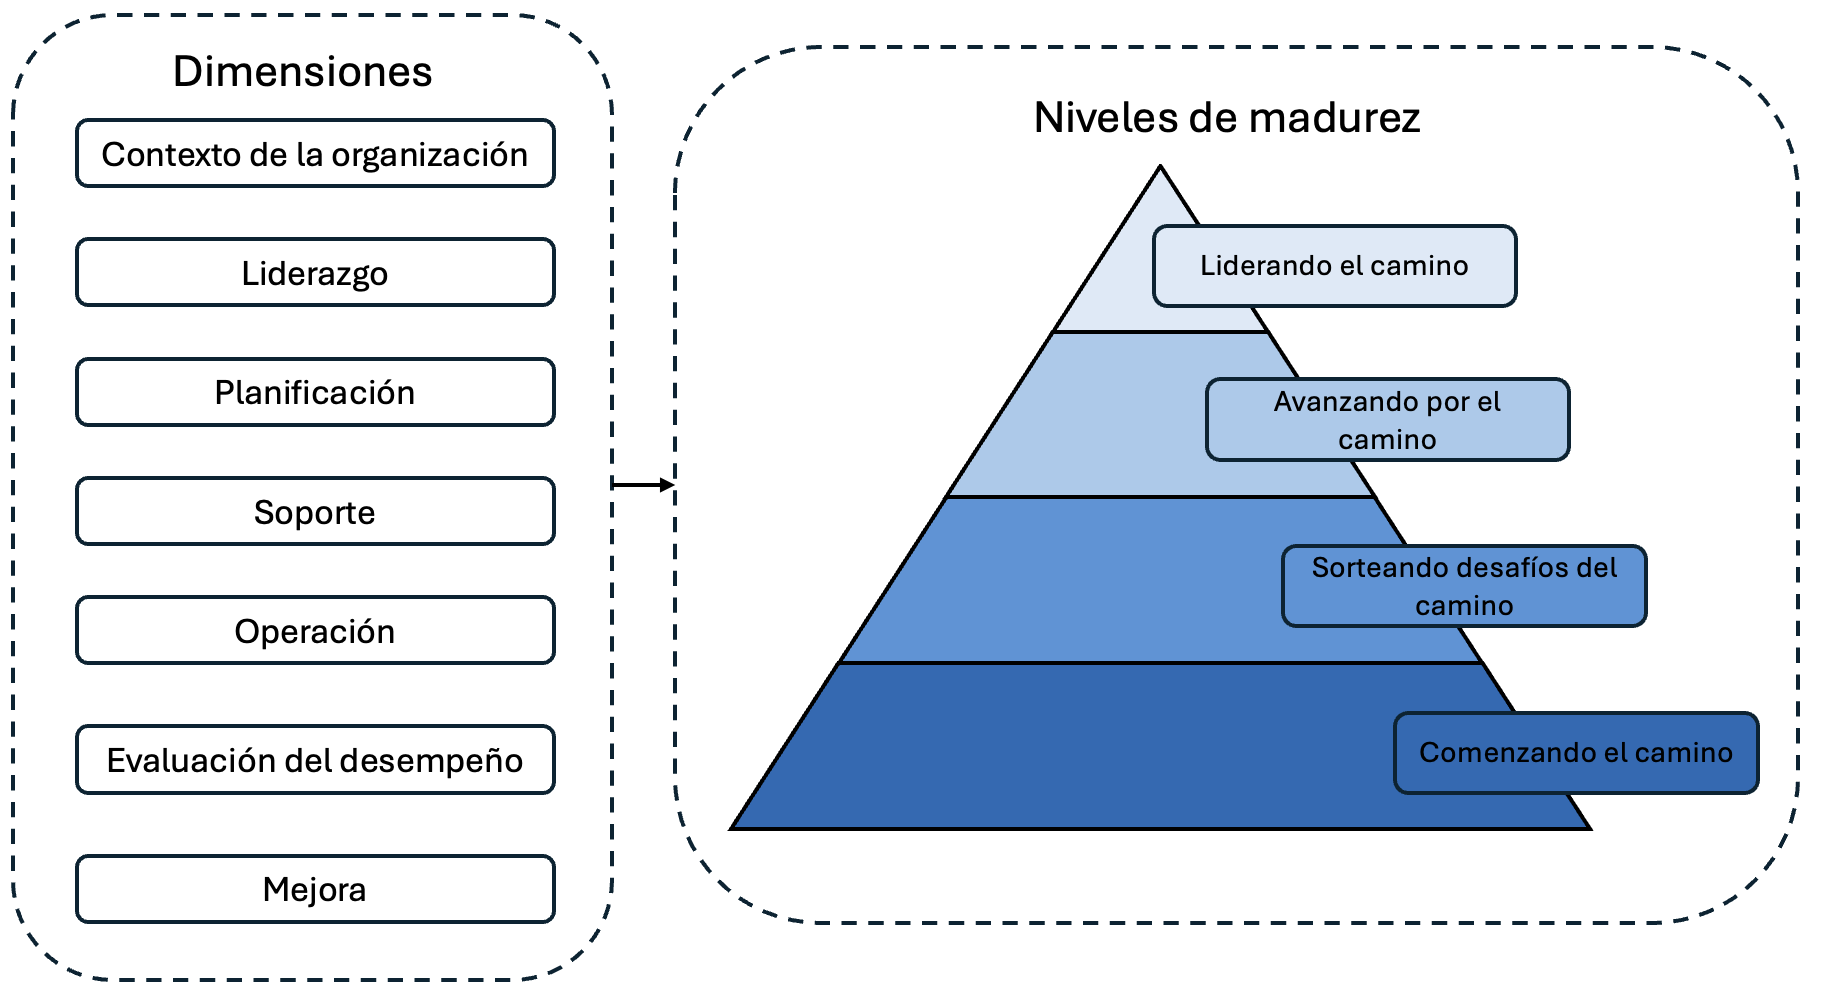
\includegraphics[scale=0.4]{images/5-implementacion/modelo-madurez.png}
    \caption{Modelo de madurez}
    \label{fig:modelo-madurez}
\end{figure}

El primer nivel del modelo de madurez de la estrategia Negocio-Agua se llama Comenzando el camino. En este nivel la empresa todavía está en etapas preliminares para lograr comprender y actuar sobre las dependencias e impactos que tiene sobre el agua. En el siguiente nivel de madurez denominado ‘Sorteando desafíos del camino’ la empresa ya ha comenzado a comprender y actuar sobre las dependencias e impactos que tiene sobre el agua, sin embargo, grandes esfuerzos se deben seguir haciendo para mejorar. En el tercer nivel de madurez, ‘Avanzando por el camino’, la empresa ya logra comprender y actuar sobre las dependencias e impactos que tiene sobre el agua casi en su totalidad. En algunos casos ya empieza hacer una referencia para otras empresas. Por último, en el nivel de madurez ‘Liderando el camino’ la empresa ya logra comprender y actuar sobre las dependencias e impactos que tiene sobre el agua en su totalidad. En la mayoría de los casos es una referencia para otras empresas, además de tener programas y proyectos adicionales a favor del agua. En la tabla a continuación se muestra el puntaje mínimo y máximo por nivel. El sistema de puntuación será explicado a lo largo de esta sección.


\begin{table}[H]
    \centering
    \begin{tabular}{p{7cm} | p{2cm} | p{2cm}}
        \textbf{Nivel} & \textbf{Mínimo} & \textbf{Máximo}\\
        \hline\hline
        Comenzando el camino & 0 & 30 \\
        \hline
        Sorteando desafíos del camino & 31 & 50\\
        \hline
        Avanzando por el camino & 51 & 75\\
        \hline
        Liderando el camino & 76 & 100 \\
        \noalign{\global\arrayrulewidth=1pt} 
        \hline
    \end{tabular}
    \caption{Puntaje mínimo y máximo por nivel de madurez}
    \label{tab:niveleles-min-max}
\end{table}

El sistema de puntos está determinado a partir de las siete dimensiones que se evalúan a la empresa. Las dimensiones fueron definidas a partir de la ISO 14001 Sistemas de Gestión Ambiental – Requisitos con orientación para su uso \parencite{iso-2015}. Como se puede ver en la Figura \ref{fig:modelo-madurez} la primera dimensión es ‘Contexto de la organización’. Esta dimensión busca comprender el contexto en el que opera la organización, incluyendo las necesidades y expectativas relacionadas con el agua como servicio ecosistémico. Es crucial para determinar los objetivos y el alcance de la gestión del agua. Luego está ‘Liderazgo’ la cual evalúa a la alta dirección\footnote{Alta dirección: persona o grupo de personas que dirige y controlan una organización al más alto nivel \parencite{iso-2015}.}. Esta debe mostrar un compromiso claro con la gestión del agua como servicio ecosistémico, estableciendo políticas y asignando responsabilidades para garantizar su efectividad. La siguiente dimensión, ‘Planificación’, evalúa establecer objetivos claros relacionados con la gestión del agua, considerando los riesgos, oportunidades y dependencias asociadas. También implica evalúa la integración de acciones específicas para alcanzar los objetivos ambientales relacionados con el agua en los procesos de negocio de la organización. La cuarta dimensión, ‘Soporte’, evalúa si la organización proporciona los recursos necesarios y se asegura de que su personal tenga las competencias adecuadas para llevar a cabo la gestión del agua como servicio ecosistémico. Además, evalúa si los canales de comunicación son efectivos interna y externamente.  Internamente hace referencia a comunicaciones que deberían ocurrir dentro de la misma empresa, mientras que, externamente hace referencia a comunicaciones con, por ejemplo, proveedores o clientes. La siguiente dimensión, ‘Operación’, hace referencia a la planificación, implementación y control de los procesos necesarios para cumplir con los requisitos de gestión del agua como capital natural, así como para responder a situaciones de emergencia relacionadas con el agua. La sexta dimensión, ‘Evaluación del desempeño’, incluye la evaluación del seguimiento, medición, análisis y evaluación del desempeño en la gestión del agua como capital natural, con revisiones periódicas por parte de la alta dirección para garantizar la eficacia continua. Finalmente, la última dimensión, ‘Mejora’, incluye la evaluación de la identificación de áreas de mejora, la implementación de acciones correctivas y preventivas, la participación en la restauración y reparación de daños al agua y los ecosistemas, así como el compromiso con la mejora continua en la sostenibilidad ambiental y la protección de los recursos hídricos.

A partir de las siete dimensiones previamente descritas se califica a la empresa para luego determinar el nivel de madurez. Cada dimensión tiene un número de preguntas que evalúan a la empresa (en la sección \ref{apx:preguntas}. \nameref{apx:preguntas} están todas las preguntas hechas con sus respuestas posibles). En la siguiente tabla se podrá ver el número de preguntas y puntos por dimensión.


\begin{table}[H]
    \centering
    \begin{tabular}{p{5cm} | p{4.5cm} | p{4.5cm}}
        \textbf{Dimensión} & \textbf{Núm. Preguntas} & \textbf{Puntos disponibles}\\
        \hline\hline
        Contexto de la organización & 12 & 20 \\
        \hline
        Liderazgo & 7 & 10 \\
        \hline
        Planificación & 13 & 31\\
        \hline
        Soporte & 12 & 22\\
        \hline
        Operación & 5 & 7\\
        \hline
        Evaluación del desempeño & 13 & 28 \\
        \hline
        Mejora & 7 & 5\\
        \hline
        \textbf{Total} &  69 & 123\\
        \hline
    \end{tabular}
    \caption{Número de preguntas y puntos disponibles por dimensión}
    \label{tab:num-preguntas-puntos-dimension}
\end{table}

Estas preguntas son de diferentes estilos, existen preguntas de si-no, escogencia única y múltiple. Cada pregunta, además, tiene la opción de No Sabe/ No responde (NS/NR) ya que esta estrategia está dirigida a una empresa genérica. El puntaje de la dimensión es determinado por la respuesta que se da en cada pregunta. Existen diferentes tipos de puntajes de preguntas. Sin embargo, para determinar el puntaje que tenía cada respuesta se pensó en la empresa ideal. Esto quiere decir, se pensaba como la empresa ideal y a partir de ahí se asignaba el puntaje. Por ejemplo, en la pregunta número 21.1, la empresa ideal debería seleccionar a todos los \textit{stakeholders} ya que en la implementación de la estrategia todo el mundo debería ser tomado en cuenta. En siguiente tabla se podrá ver los tipos de preguntas y sus sistemas de calificación. 


\begin{table}[H]
    \centering
    \begin{tabular}{p{5cm} | p{8cm}}
        \textbf{Nombre} & \textbf{Descripción}\\
        \hline\hline
        Binario & Solo una de las opciones disponibles da puntos \\
        \hline
        Si Sabe/Si Responde & Si la respuesta no es NS/NR dará un punto\\
        \hline
        Suma & El número de opciones seleccionadas, que no sean NS/NR, dará puntos.\\
        \hline
        Mejor & Entre todas las opciones existen opciones con más y menos puntos\\
        \hline
        No Puntos & Ninguna opción de la pregunta dará puntos\\
        \hline
    \end{tabular}
    \caption{Tipo de pregunta y su sistema de calificación}
    \label{tab:pregunta-calificacion}
\end{table}

\subsubsection{Metodología: \textit{Analytic Hierarchy Process}}
Luego de tener el puntaje por dimensión para determinar el nivel de madurez, se aplica una ponderación. Esta ponderación se basa en la importancia relativa de cada dimensión en la determinación del nivel de madurez. Es decir, a cada dimensión se le asigna un porcentaje (peso) para determinar el puntaje final. Este peso se determinó utilizando la metodología \textit{Analytic Hierarchy Process} \parencite{bahurmoz-2006}.

La metodología del Proceso Analítico Jerárquico (AHP) es un enfoque estructurado para la toma de decisiones que ayuda a descomponer problemas complejos en componentes más manejables, establecer prioridades y tomar decisiones racionales. Se basa en la comparación de criterios y alternativas a través de matrices de comparación, lo que permite asignar pesos a los criterios y tomar decisiones fundamentadas. 

Para obtener los pesos por dimensión se realizó un taller con cuatro expertos en donde se determinada la importancia relativa. El objetivo de este taller es establecer la importancia de las dimensiones que determinan el nivel de la empresa con respecto a sus dependencias e impactos sobre el agua. La importancia será determinada haciendo una comparación entre cada dimensión. Es decir, la importancia de la 'Dimensión A' relativa a la 'Dimensión B'. A continuación, se puede ver una matriz ejemplo del taller.

\begin{figure}[H]
    \centering
    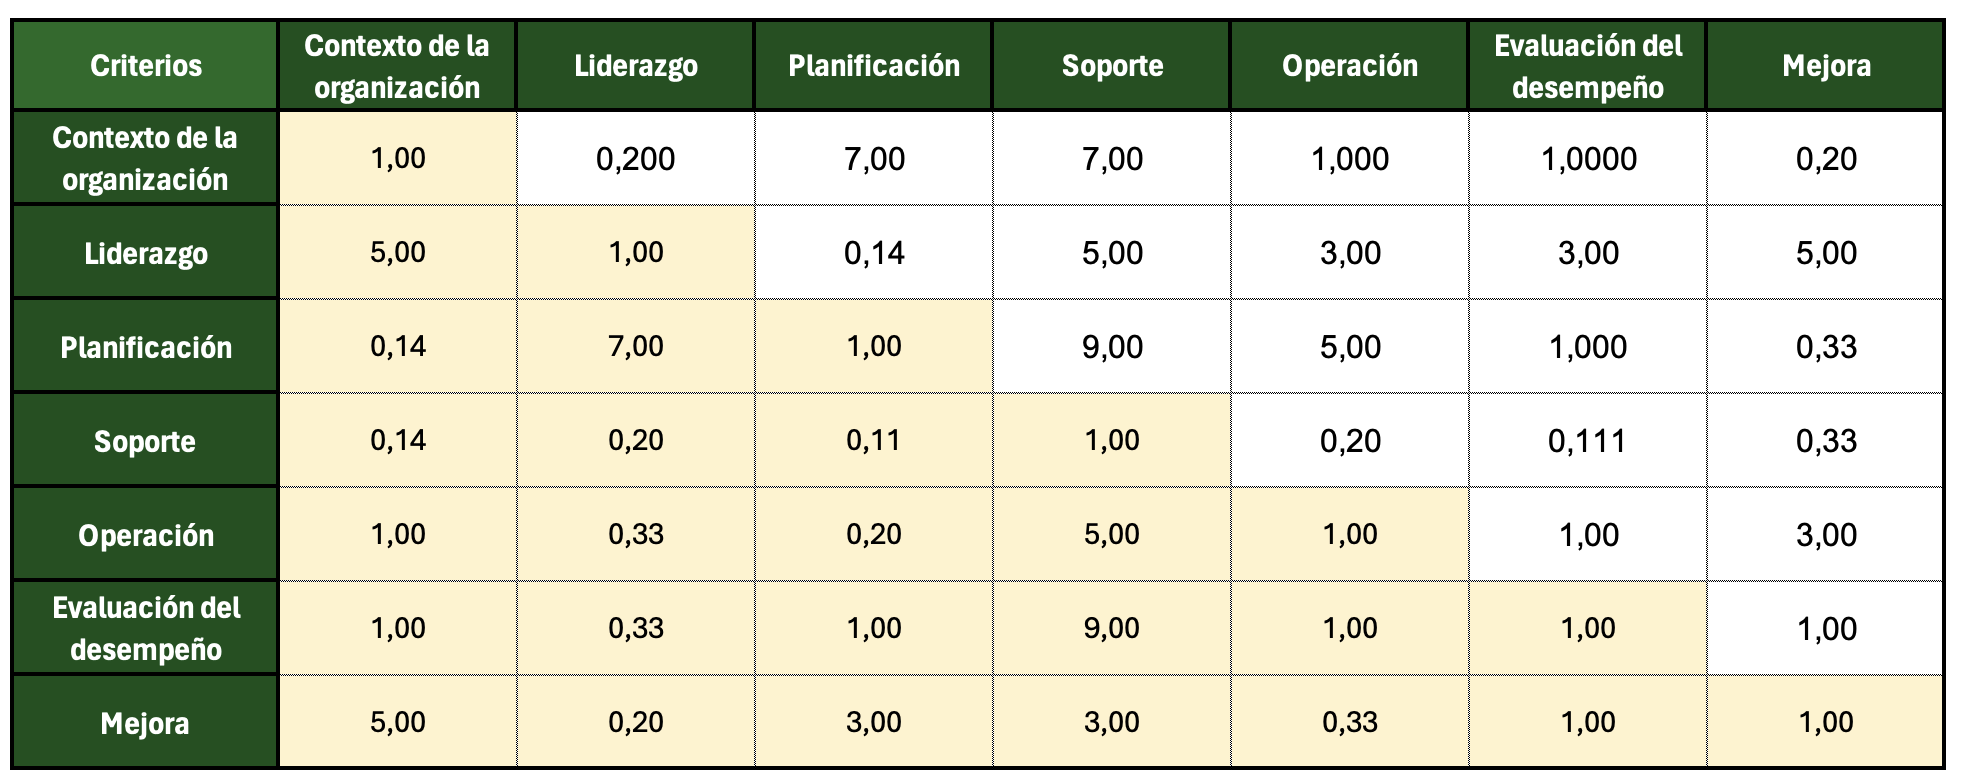
\includegraphics[scale=0.45]{images/5-implementacion/ejemplo-matriz.png}
    \caption{Ejemplo de matriz realizada por experta M.A. Parra}
    \label{fig:ejemplo-matriz}
\end{figure}

Las comparaciones se hacen Fila 1 vs Todas las columnas, luego Fila 2 vs Todas las columnas, etc.  Para determinar la importancia la matriz se lee tal que se haga la pregunta: "¿Qué tan importante es la dimensión i (fila) con respecto a la dimensión j (columna)?". La importancia entre dos dimensiones se determina de la siguiente manera: si es igual de importante = 1; si es levemente más importante = 3; si es mucho más importante = 5; si es demasiado más importante = 7; si es extremadamente más importante = 9. Si el experto cree que la importancia de la dimensión de la fila 1 es menor por un grado N relativa a alguna columna, entonces coloque en la celda correspondiente 1/N. Para obtener los pesos definitivos por dimensión se hizo el promedio de los pesos por dimensión. A continuación, podrá ver los resultados del taller y los pesos por dimensión.


\begin{table}[H]
    \centering
    \begin{tabular}{p{5cm}|p{1.25cm}|p{1.25cm}|p{1.25cm}|p{3.25cm}}
        \textbf{Dimensión} & \textbf{Exp 1} & \textbf{Exp 2} & \textbf{Exp 3} & \textbf{Peso Definitivo} \\
        \hline\hline
        Contexto de la organización & 17\% & 11\% & 34\% & 21\%\\
        \hline
        Liderazgo & 21\% & 25\% & 13\% & 20\%\\
        \hline
        Planificación & 27\% & 13\% & 14\% & 18\%\\
        \hline
        Soporte & 2\% & 18\% & 7\% & 9\%\\
        \hline
        Operación & 8\% & 6\% & 20\% & 11\%\\
        \hline
        Evaluación del desempeño & 11\% & 6\% & 6\% & 8\%\\
        \hline
        Mejora & 14\% & 20\% & 6\% & 14\%\\
        \hline
    \end{tabular}
    \caption{Pesos relativos de las dimensiones por experto}
    \label{tab:pesos-expertos}
\end{table}

\subsubsection{Sistema de puntos}
Luego de obtener los puntos y los pesos relativos por dimensión se puede proceder a obtener el puntaje final que determina el nivel de madurez. En la Ecuación \ref{eq:nivel-madurez} se puede ver cómo se obtiene el puntaje.

\begin{equation} \label{eq:nivel-madurez}
P = (\sum_{i=1}^{7} d_i/t_i \times p_i) \times 100
\end{equation} 

El puntaje final, $P$, es igual a la suma del porcentaje de  puntos obtenidos de cada dimensión $i$, $d_i/t_i$, ponderado por el peso de misma la dimensión, $p_i$. La variable $d_i$ corresponde a los puntos obtenidos en la dimensión $i$, mientras que la variable $t_i$ es la cantidad de puntos posibles de la dimensión $i$.

\subsubsection{Relación entre el negocio y el agua}
Además de determinar el nivel de madurez de una empresa, la estrategia también busca concientizar a las empresas sobre sus actuales relaciones con el agua. Estas relaciones se basan en los indicadores que la empresa actualmente mide o contempla en los reportes que realiza acerca del agua como capital natural dentro de su negocio. En específico, con qué SSEE, funciones y gestiones ecosistémicas se relacionan los indicadores de la empresa. Estas relaciones fueron determinadas por los expertos M.A. Parra y M. Murcia, los cuales utilizaron las siguientes referencias: \textit{Guidelines for identifying business risks and opportunities arising from ecosystem change: Version 2.0} (Hanson et al., 2012) y \textit{A typology for the classification, description and valuation of ecosystem functions, goods and services} (De Groot et al., 2002). Los expertos fundamentaron sus respuestas en estas dos referencias debido al elevado nivel de aceptación que tienen en la industria y a su amplia citación en diversos artículos. El objetivo principal de establecer estas relaciones es poder concientizar a las empresas de que los procesos que ellos realizan tienen dependencias y generan impactos sobre los SSEE, funciones y procesos ecológicos asociados al agua.  En la sección de Anexos, podrá encontrar los indicadores y sus respectivas relaciones. 

Establecer las relaciones entre el negocio y el agua, en especial entre los indicadores que utiliza la empresa y las gestiones ecosistémicas cobra importancia en Colombia para seguir la \acrfull{pngibse}. Según el \textcite{ministerio-de-ambiente-y-desarrollo-sostenible-2012},

\hfill
\par
\leftskip=0.35in \rightskip=0.35in
\acrshort{pngibse} será la que enmarque y oriente conceptual y estratégicamente todos los demás instrumentos ambientales de gestión (políticas, normas, planes, programas y proyectos), existentes o que se desarrollen, para la conservación de la biodiversidad en sus diferentes niveles de organización, además de ser base de articulación intersectorial y parte fundamental en el desarrollo del país.

\hfill
\par
\leftskip=0in \rightskip=0in
Es por esto por lo que es muy importante que las empresas entiendan y conozcan las relaciones que existen entre su negocio y los diferentes componentes del ecosistema. Esto incluye, además, todos los capitales naturales, SSEE, funciones ecosistémicas, etc. Entendiendo estas relaciones, va a ser la forma principal en la que las empresas podrán seguir mejorando sus estados actuales. Además, podrá minimizar los costos adicionales generados por reparaciones y daños, si desde un principio entienden las relaciones tal que puedan seguir las políticas, normas, planes, programas y proyectos. 

\subsubsection{Indicadores}
Además de establecer las relaciones con el agua, los indicadores también son una fuente de información para evaluar una empresa (\ref{apx:indicadores}. \nameref{apx:indicadores}). En especial, evaluar los datos y las fuentes de información y la calidad de los atributos que mide las empresas. Para esto, la estrategia evalúa la granularidad, frecuencia, comparabilidad, fuente, tipo, \textit{Sciene Based Target} (SBT)\footnote{\textit{Science Based Target}: Los objetivos basados en la ciencia proporcionan una vía claramente definida para que las empresas reduzcan las emisiones de gases de efecto invernadero (GEI), ayudando a prevenir los peores impactos del cambio climático y el crecimiento empresarial a prueba de futuro \parencite{science-based-targets-no-date}.} y validación externa. En la siguiente tabla se podrá ver las preguntas que se hacía por atributo de calidad del indicador y sus opciones.


\begin{table}[H]
    \centering
    \begin{tabular}{p{3cm} | p{7cm} | p{4.5cm}}
        \textbf{Dimensiones} & \textbf{Pregunta} & \textbf{Opciones} \\
        \hline\hline
        Granularidad & Seleccione el nivel de granularidad de los datos&País-Departamento-Municipio-Cuenca-NS/NR\\
        \hline
        Frecuencia & Seleccione la frecuencia de los datos utilizados para armar/calcular los indicadores&Diaria-Semanal-Mensual-Bimestral-Semestral-Anual-NS/NR\\
        \hline
        Comparabilidad & ¿Sus datos han sido comparados con otros datos externos?&SI-NO-NS/NR\\
        \hline
        Fuente & ¿Cuál es la fuente principal de los datos utilizados para armar/calcular los indicadores?& Datos primarios-Datos secundatios-NS/NR\\
        \hline
        Tipo & ¿Qué tipo de indicador es?&Cualitativo-Cuantitativo-NS/NR\\
        \hline
        SBT & ¿Sus datos son \textit{Science Based Targets} (SBT)?& SI-NO-NS/NR\\
        \hline
    \end{tabular}
    \caption{Atributos evaluados de los indicadores}
    \label{tab:atributos-indicadores}
\end{table}

\subsubsection{Servicios Ecosistémicos}
La estrategia también le permite a la empresa que tiene un mayor grado de conocimiento evaluar las dependencias e impactos sobre los servicios ecosistémicos asociados a los indicadores medidos. Esto permite una mayor profundización en la estrategia y, además, a aquellas empresas que no sabían acerca del nivel de dependencia (bajo, medio o alto) y el tipo de impacto (positivo o negativo) que tenían sobre los servicios ecosistémicos asociados a los indicadores medido o contemplados, les hace reflexionar y enterarse de información que deberían tener en cuenta. 


\subsection{Implementación y desarrollo de la herramienta} \label{subsec:implementacion-desarrollo-herramienta}

En esta sección se explicará el desarrollo e implementación del modelo generado por la estrategia en una herramienta que permita determinar el nivel de madurez de la empresa, al mismo tiempo que se visualiza su relación con el agua a partir de la información proporcionada por la misma empresa. La herramienta se desarrolló en una aplicación web que utiliza MongoDB para almacenar los datos, Render para desplegar la aplicación y Dash Plotly como librería principal de Python para crear la aplicación y sus servicios. En el siguiente diagrama se podrá ver la relación entre los componentes previamente mencionados. 

\begin{figure}[H]
    \centering
    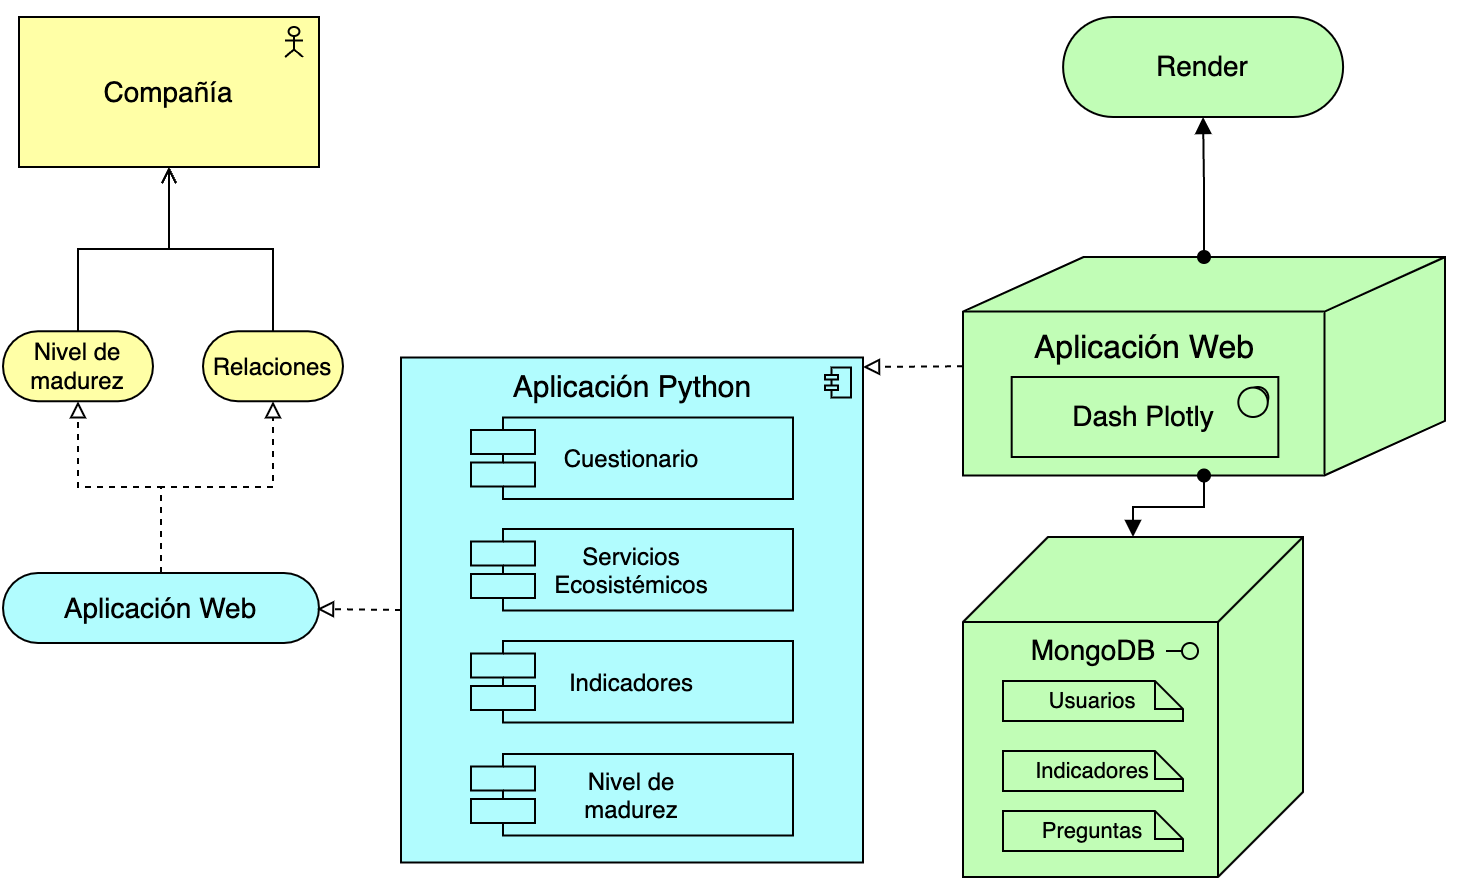
\includegraphics[scale=0.45]{images/5-implementacion/diagrama-archimate.png}
    \caption{Diagrama archimate de la aplicación web}
    \label{fig:archimate-app-web}
\end{figure}

A través de una serie de preguntas, se buscará determinar el nivel de madurez de la empresa con respecto a las dependencias e impactos que tiene sobre el agua. La aplicación web tiene los siguientes objetivos:

\begin{enumerate}
    \item Determinar el nivel de madurez a partir de la evaluación del conocimiento y acciones que tiene la empresa acerca de las dependencias y los impactos sobre el agua.
    \item Entender, de las dimensiones a evaluar, cuál es la mejor dimensión actualmente que tiene la empresa.
    \item Exponer a la empresa, según los indicadores que miden, cuáles servicios y funciones ecosistémicos deben contemplar en los reportes relacionados con el agua.
\end{enumerate}

En la Figura \ref{fig:paso-paso-app} se puede ver el paso a paso de cómo se pueden cumplir con los tres objetivos anteriormente mencionados. En el primer paso, ‘Cuestionario’, la empresa deberá responder un conjunto de preguntas relacionadas a los conocimientos y acciones que actualmente está haciendo en relación con las dependencias e impactos sobre el agua. En el siguiente paso, ‘Indicadores’, la empresa deberá seleccionar los indicadores que actualmente estén midiendo o contemplando en reportes relacionados al agua. Luego, en el paso ‘Nuevos indicadores’, la empresa podrá ingresar sus propios indicadores, que no encontró en la anterior sección, a la herramienta. A partir del segundo paso, en el paso ‘Servicios Ecosistémicos, la empresa podrá determinar el nivel de dependencia (bajo, medio, alto) y el tipo de impacto (positivo, negativo) que tiene sobre los servicios ecosistémicos. En el quinto paso, ‘Funciones Ecosistémicas’, la empresa podrá ver una visualización de la relación entre indicadores, servicios y funciones ecosistémicos, para entender la importancia en la relación entre el negocio y el agua y sus servicios ecosistémicos. Finalmente, en el último paso, ‘Resultados’, la empresa podrá saber cuál es su nivel de madurez, su puntaje obtenido, su mejor dimensión, el puntaje y descripción por dimensión y unas gráficas descriptivas para los indicadores escogidos. En la sección \ref{apx:imagenes-app-web}. \nameref{apx:imagenes-app-web}, están las imágenes para cada uno de los pasos anteriormente mencionados.

\begin{figure}[H]
    \centering
    
\includegraphics[scale=0.4]{images/5-implementacion/paso-a-paso-app.png}
    \caption{Paso a paso de la aplicación}
    \label{fig:paso-paso-app}
\end{figure}

En la Figura \ref{fig:resultados-nivel-madurez} se ve un resultado ejemplo de la aplicación. En la primera fila, luego del encabezado, se ven los tres primeros resultados. El primer (1) resultado muestra el nivel de madurez obtenido, en este caso 'Sorteando desafíos del camino'. El siguiente resultado (2) muestra el puntaje obtenido, el cual define el nivel de madurez mencionado. El tercer (3) resultado en esta fila muestra la mejor dimensión obtenida por la empresa ('Contexto de la organización').

\begin{figure}[H]
        \centering
        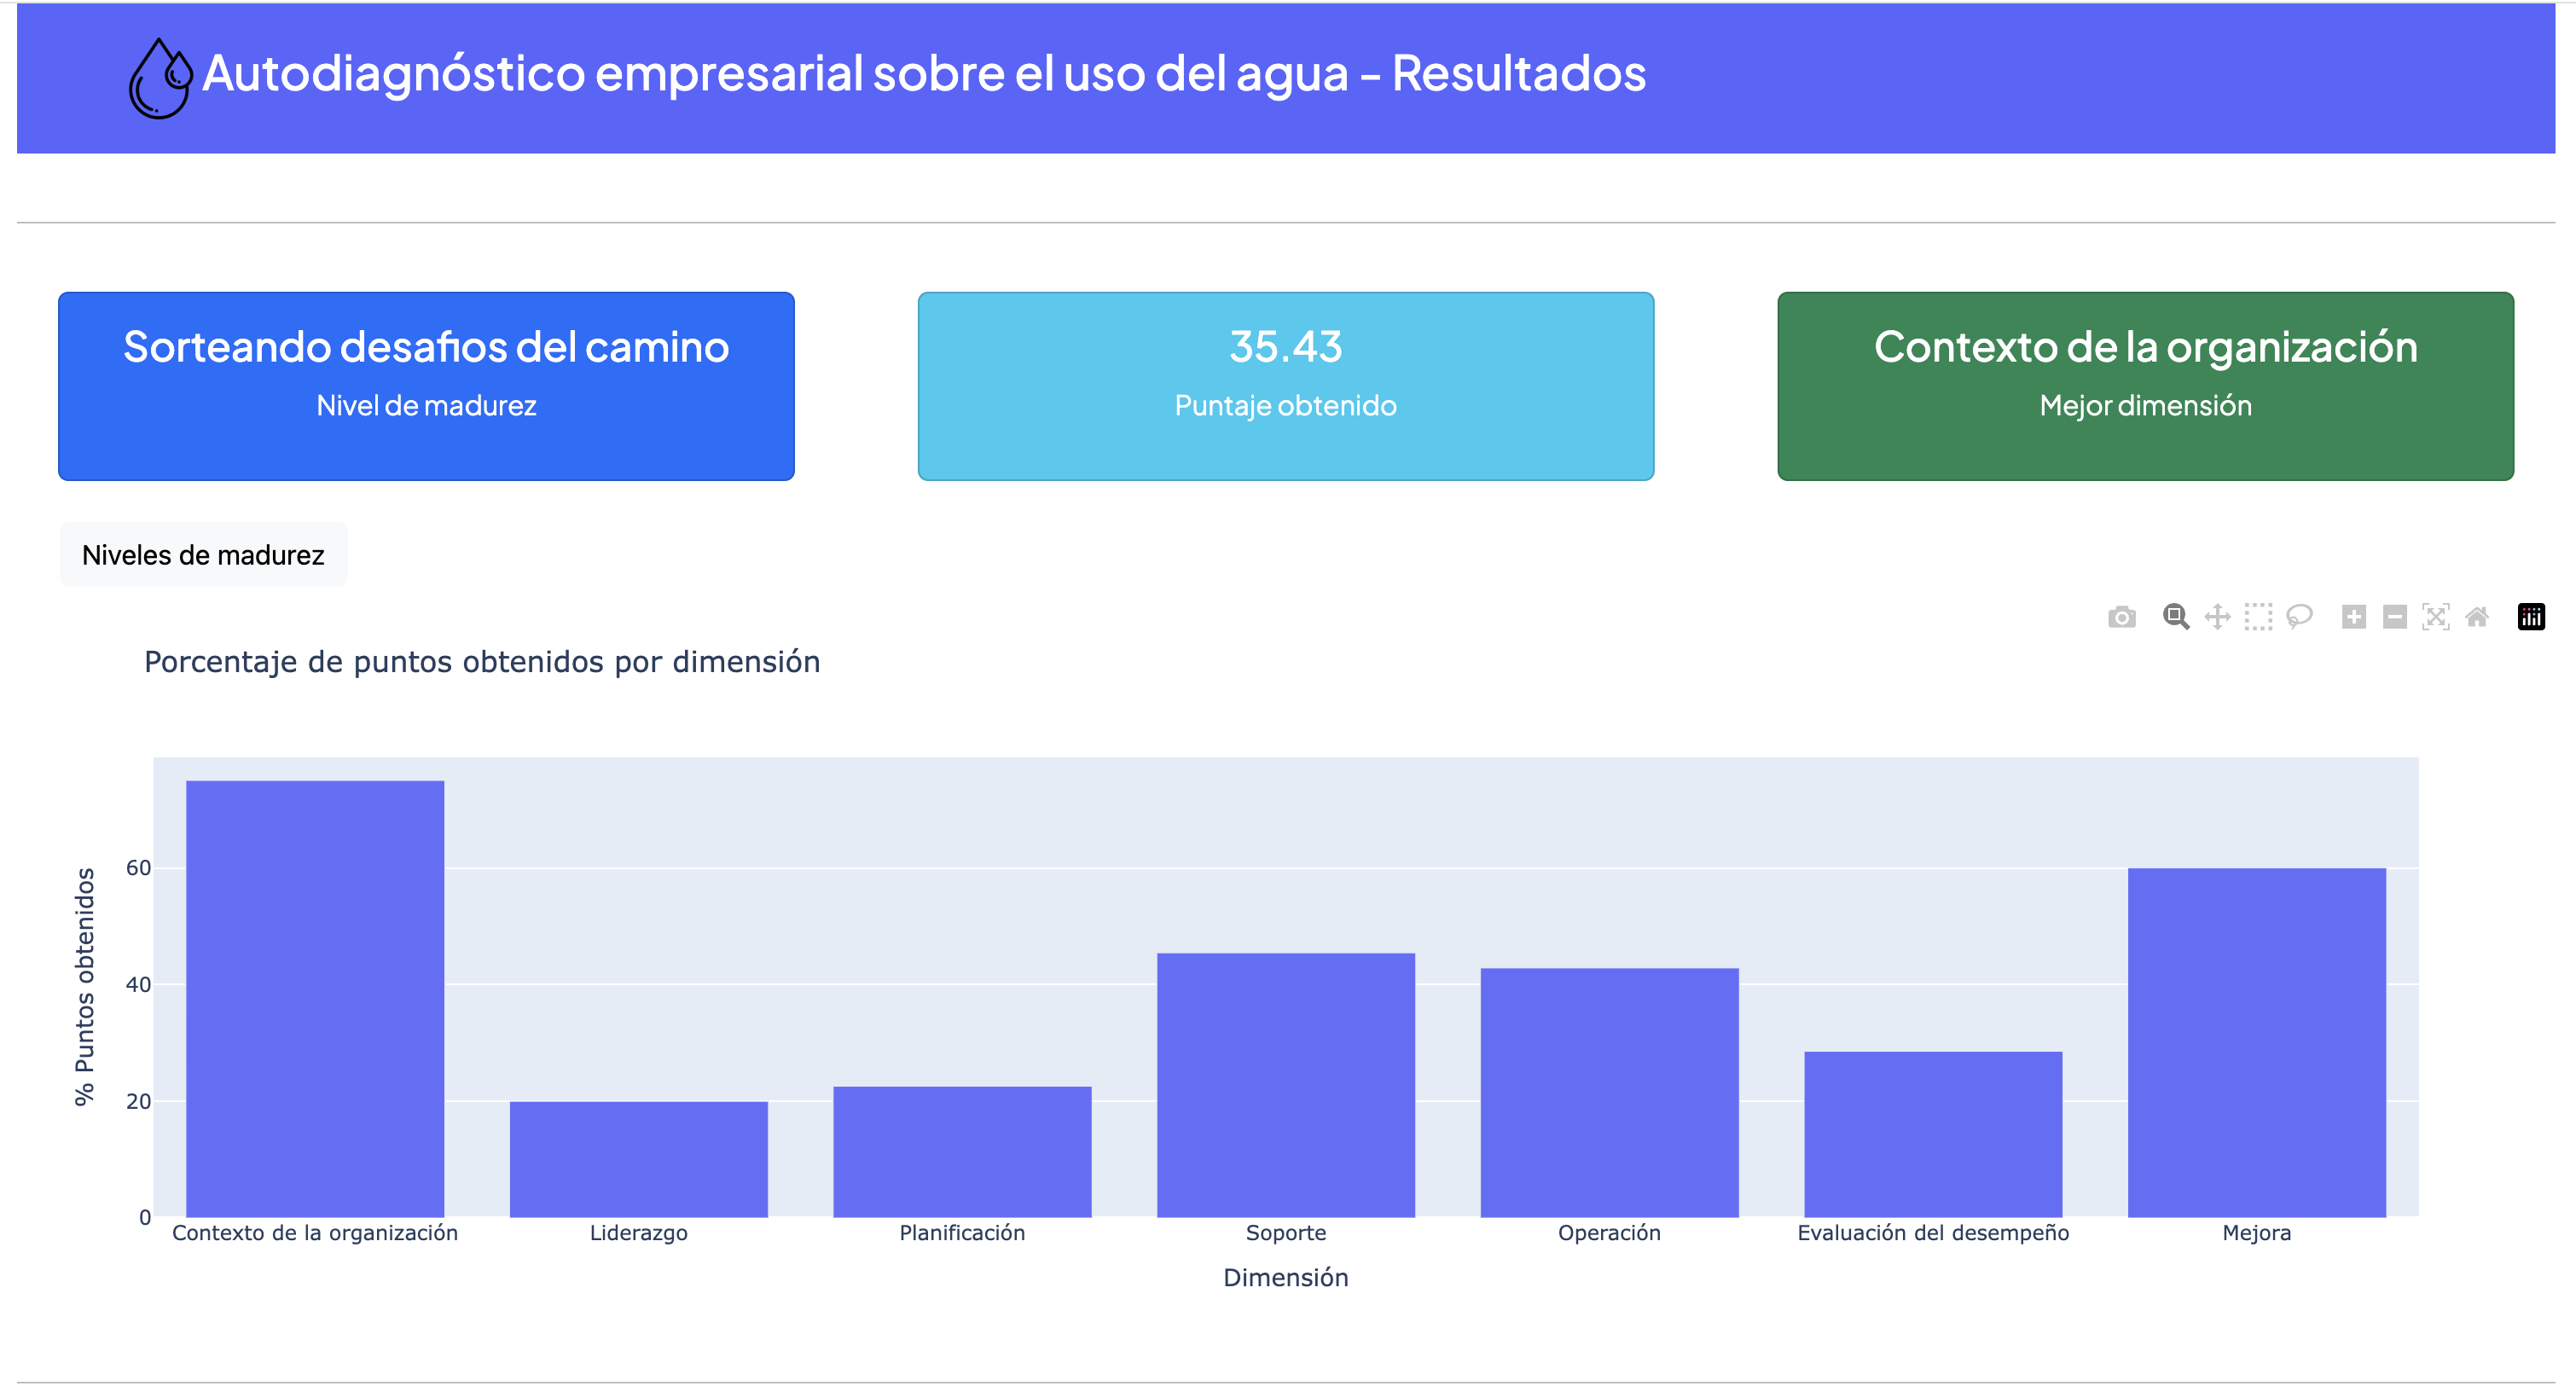
\includegraphics[scale=0.25]{images/99-aplicacion-web/8-mm.png}
        \caption{Resultado-Nivel de madurez de la empresa}
        \label{fig:resultados-nivel-madurez}
\end{figure}

En la gráfica dentro de la Figura \ref{fig:resultados-nivel-madurez}, se observa el porcentaje de puntos obtenidos (eje vertical) para cada dimensión (eje horizontal). Para el 'Contexto de la organización', se obtuvo alrededor del 70\% de los puntos. Esto indica que la empresa conoce su estado actual y sus necesidades; sin embargo, podría mejorar en la determinación de los objetivos y el alcance de la gestión del agua de manera correcta. En la dimensión 'Liderazgo', se evidencia que la alta dirección no muestra un compromiso claro con la gestión del agua, ya que no establece políticas ni asigna responsabilidades para garantizar su efectividad. De manera similar, en la dimensión 'Planificación', con un bajo porcentaje de puntos obtenidos (aproximadamente 23\%), los objetivos no se establecen claramente en relación con la gestión del agua, considerando los riesgos, oportunidades y dependencias asociadas. Para la dimensión 'Soporte', con alrededor del 45\% de los puntos posibles, la empresa debe asegurar que su personal tenga mayores competencias y mejores recursos para llevar a cabo la gestión del agua como servicio ecosistémico. Además, debe establecer canales de comunicación efectivos, tanto internos como externos, relacionados con la gestión del agua. En la dimensión 'Operación', al obtener casi el 42\% de los puntos posibles, la empresa necesita mejorar significativamente en la planificación, implementación y control de los procesos necesarios para cumplir con los requisitos de gestión del agua como servicio ecosistémico, así como en la respuesta a situaciones de emergencia relacionadas con el agua. Según la gráfica, la empresa tiene mucho por mejorar en el seguimiento, medición, análisis y evaluación del desempeño en la gestión del agua, con revisiones periódicas por parte de la alta dirección para garantizar la eficacia continua, ya que obtuvo solamente el 30\% de los puntos posibles en la dimensión 'Evaluación del desempeño'. Finalmente, la empresa debe mejorar sustancialmente en la identificación de áreas de mejora, implementación de acciones correctivas y preventivas, y debe tener una mayor participación en la restauración y reparación de daños al agua y los ecosistemas ya que obtuvo el 50\% de los puntos posibles. 



\section{Validación}
\subsection{Métodos}
La validación realizada para este proyecto consistió en una encuesta que debe contestar dos expertos y una empresa. Los dos expertos son Mario Murcia y María Angélica Parra, los dos son expertos en temas relacionados con los ecosistemas y el agua. Por otro lado, la empresa que ha validado la herramienta desarrollada es Corona, en especial la división independiente de Corona, Empresa Colombiana de Cementes (Alion). Alion es una división independiente de Corona cuyo origen es una alianza con Cementos Molins de España. Esta división comenzó operaciones en el 2019-2 y se especializa en la extracción de caliza en Río Claro. Alion es el proveedor principal de insumos de otras divisiones de Corona como, por ejemplo, Insumos Industrias y Energía. 
Para la validación de la aplicación web, proveniente del modelo producto de la estrategia, se realizó un formulario en Google Forms. Este formulario busca evaluar los atributos de calidad de la aplicación web, la calidad de preguntas con respecto al contexto del agua como capital natural y otros atributos que se deben evaluar de la aplicación. En la tabla \ref{tab:formulari-validacion} en el Apéndice A podrá ver las preguntas que se realizaron en el formulario. Por cada atributo evaluado se incluyó una sección abierta para que el evaluador pudiera incluir comentarios adicionales.

Las preguntas relacionadas al contexto, practicidad, visualizaciones finales y utilidad están evaluando de manera indirecta a la estrategia. Esto se debe a que están evaluando la calidad del modelo, la facilidad de usar la herramienta y por lo tanto la estrategia, la claridad de las visualizaciones finales, i.e., los resultados de la estrategia y la utilidad de la herramienta, es decir, si los resultados han ayudado a la empresa a entender su situación actual.

\subsection{Validación de resultados}
En esta sección se discutirá los resultados de las validaciones hechas por los expertos. Los cuatro atributos de calidad evaluados de la aplicación web fueron la funcionalidad, la confiabilidad, la usabilidad y el rendimiento. En la segunda pregunta relacionada a la funcionalidad de la herramienta, “¿Encontró alguna función que no estuviera disponible y que considere esencial?”, hubo un comentario que mencionaba que hacía falta el servicio ecosistémico ‘Cultural del Agua’. Este error pudo haber sido causado por una falta de atención en el momento de copiar la información entregada por el experto a la aplicación.  En esta sección también se hizo el comentario de una mayor explicación en la sección de indicadores puesto que la búsqueda en los documentos de estos no es inmediata y se puede caer en imprecisiones. En la siguiente imagen se podrá ver las respuestas a la primera pregunta de la validación. Como se puede ver, tanto a los expertos como a la empresa, estaban todas las necesidades para evaluar las dependencias e impactos de la empresa sobre el agua.

\begin{figure}[H]
        \centering
        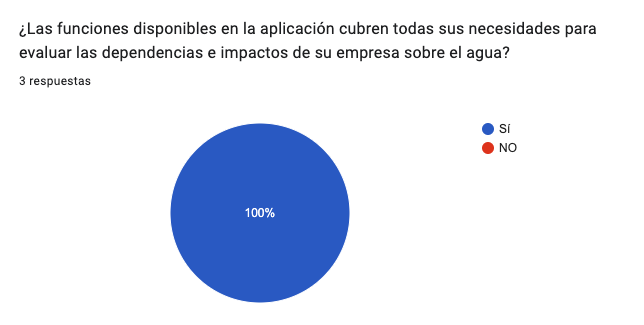
\includegraphics[scale=0.45]{images/6-validacion/1-funcionalidad.png}
        \caption{Respuestas de la primera pregunta relacionada a la funcionalidad de la aplicación web}
 \end{figure}

Con respecto a la confiabilidad, el único comentario que se obtuvo fue que la aplicación permitía continuar a la siguiente pregunta sin haber respondido la pregunta. Este comportamiento está basado en el comportamiento de la herramienta de IMPULS Industry 4.0 Readiness Online Self-Check for Business, la cual le permite a las empresas hacer todo el diagnóstico sin haber respondido todas las preguntas. Por otro lado, en ninguna de las validaciones hechas por los usuarios hubo pérdida de datos o información incorrecta al usar la aplicación.

\begin{figure}[H]
        \centering
        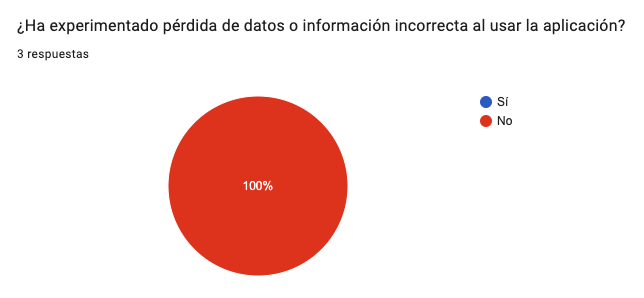
\includegraphics[scale=0.45]{images/6-validacion/2-confiabilidad.png}
        \caption{Porcentaje de pérdida de datos o información según evaluadores}
\end{figure}

La ‘Usabilidad’ de la herramienta tuvo un gran resultado pues los evaluadores se demoraron menos de 30 minutos en familiarizarse con el uso de la aplicación y el 66\% de los evaluadores consideraron la interfaz intuitiva y fácil de usar. Sin embargo, los comentarios si mencionaban como era importante advertir a la empresa que utilice la herramienta la necesidad de tener la información lista o saber dónde está para así agilizar el proceso.  Adicionalmente, se recomienda disminuir el número de preguntas para hacer el tiempo de respuesta mucho menor.

\begin{figure}[H]
        \centering
        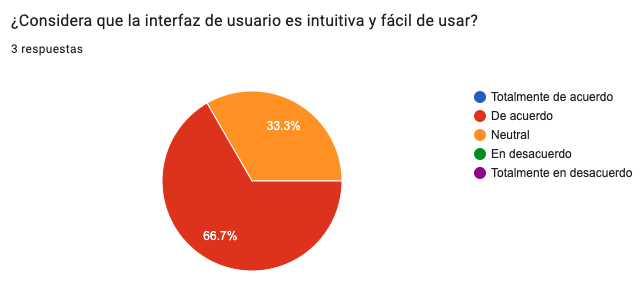
\includegraphics[scale=0.45]{images/6-validacion/3-usabilidad.png}
        \caption{Porcentaje de evaluadores que consideran la interfaz intuitiva y fácil de usar}
\end{figure}

\begin{figure}[H]
        \centering
        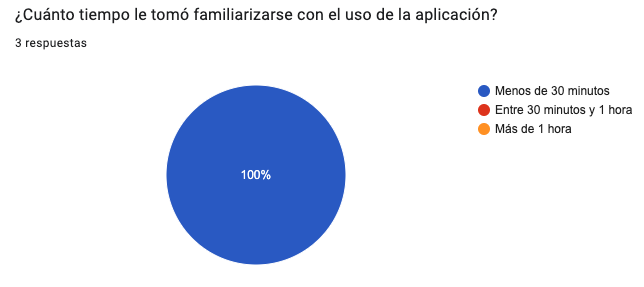
\includegraphics[scale=0.45]{images/6-validacion/4-usabilidad.png}
        \caption{Tiempo para familiarizarse con la aplicación según evaluadores}
\end{figure}
    
El rendimiento de la aplicación tuvo, en términos generales, una respuesta positiva ya que la velocidad de carga fue, por lo menos, satisfactoria. Pero, si hubo un comentario en el cual se mencionaba que había preguntas que se demoraban en salir lo que posiblemente dejaba preguntas sin responder. 

\begin{figure}[H]
        \centering
        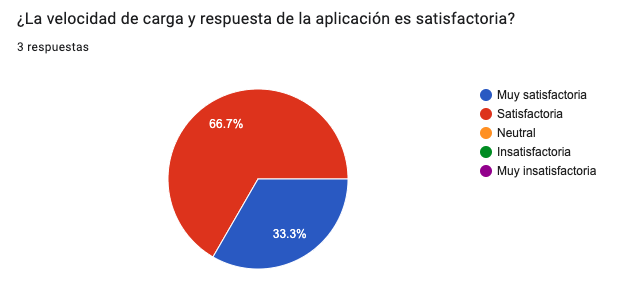
\includegraphics[scale=0.45]{images/6-validacion/5-rendimiento.png}
        \caption{Satisfacción de los evaluadores con respecto a la velocidad de carga y respuesta de la aplicación}
\end{figure}
 
\begin{figure}[H]
        \centering
        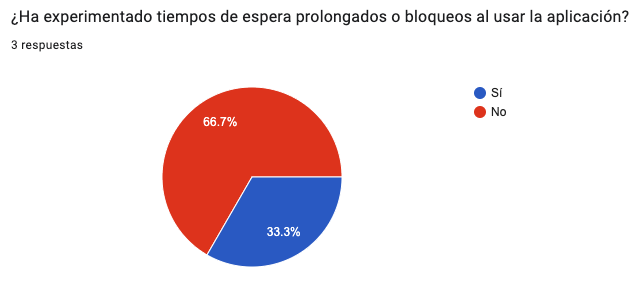
\includegraphics[scale=0.45]{images/6-validacion/6-rendimiento.png}
        \caption{Respuestas con respecto al rendimiento de la aplicación}
\end{figure}
 
  
Con respecto a la consideración del ‘Contexto’, la aplicación puede mejorar en la información mínima para que la empresa pueda entender su nivel de madurez. Adicionalmente, se puede mejorar la redacción de algunas de las preguntas hechas en el cuestionario. Finalmente, en la sección de comentarios se advierte de que la herramienta es útil para empresas reguladas, pero para empresas no reguladas podría ser un reto responder la mayoría de las preguntas. 

\begin{figure}[H]
        \centering
        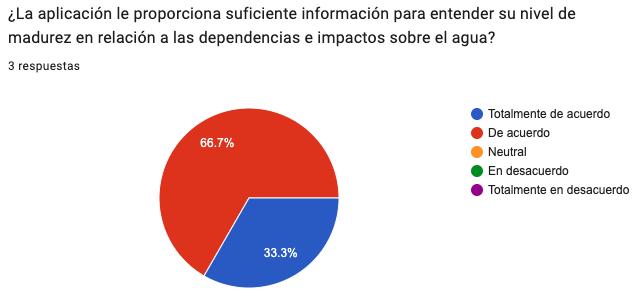
\includegraphics[scale=0.45]{images/6-validacion/7-contexto.png}
        \caption{Percepción de los evaluadores con respecto a la cantidad de información proporcionada por la aplicación para entender el nivel de madurez}
\end{figure}

\begin{figure}[H]
        \centering
        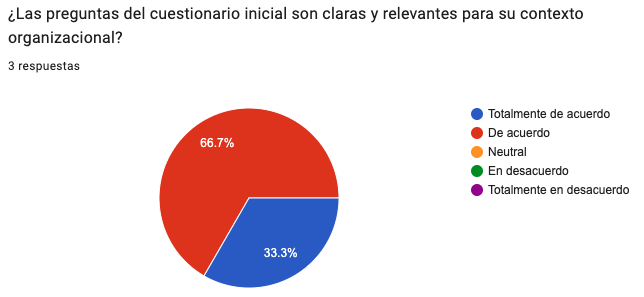
\includegraphics[scale=0.45]{images/6-validacion/8-contexto.png}
        \caption{Claridad y relevancia de las preguntas del cuestionario según los evaluadores}
\end{figure}


Para las visualizaciones finales de la aplicación donde se muestra el nivel de madurez y las relaciones el comentario principal fue la necesidad de simplificar las gráficas. Ya sea través de explicaciones más claras de cómo utilizar las gráficas o cambiar el tipo de gráficas que se utilizan. Esta inconformidad se puede ver en las gráficas presentadas a continuación. En especial, en la gráfica que muestra los resultados de la pregunta que evalúa la utilidad para los análisis de las gráficas. 


\begin{figure}[H]
        \centering
        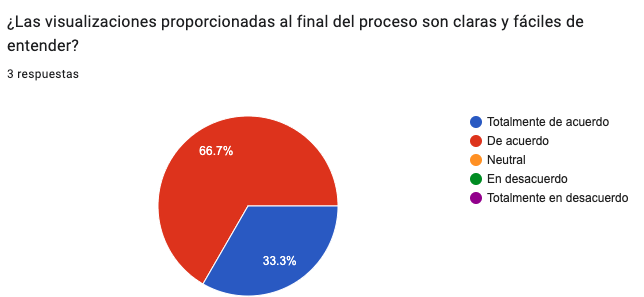
\includegraphics[scale=0.45]{images/6-validacion/9-vf.png}
        \caption{Claridad y facilidad de entender de las visualizaciones según los evaluadores}
\end{figure}
    
\begin{figure}[H]
        \centering
        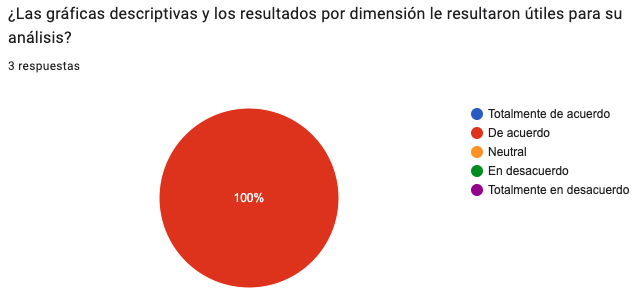
\includegraphics[scale=0.45]{images/6-validacion/10-vf.png}
        \caption{Gráficas descriptivas para entender los resultados relacionados a las dimensiones evaluadas}
\end{figure}

 

La utilidad de la aplicación tuvo grandes resultados ya que la aplicación le ha ayudado a identificar nuevas áreas de mejora en la gestión del agua al tiempo que cumple con los objetivos establecidos.  A través de la aplicación, según los evaluadores, se pudo determinar el nivel de madurez, la mejor dimensión y exponer características descriptivas de los indicadores.

\begin{figure}[H]
        \centering
        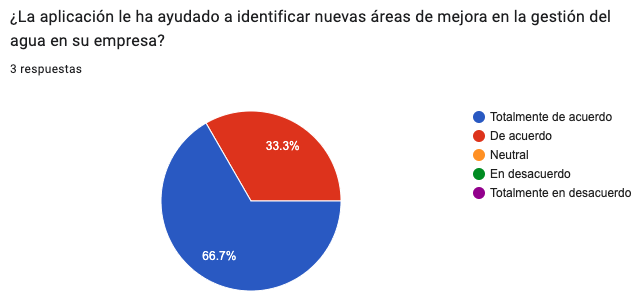
\includegraphics[scale=0.45]{images/6-validacion/11-utilidad.png}
        \caption{Utilidad para encontrar nuevas áreas de mejora}
\end{figure}

\begin{figure}[H]
        \centering
        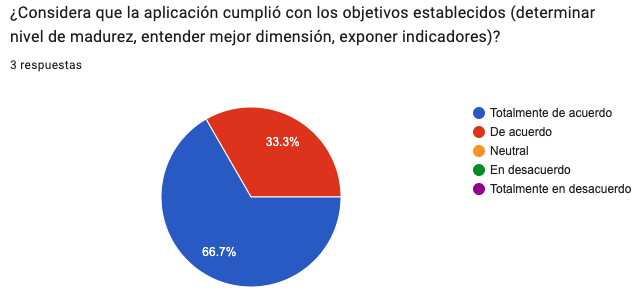
\includegraphics[scale=0.45]{images/6-validacion/12-utilidad.png}
        \caption{Percepción de los evaluadores acerca del cumplimiento de los objetivos}
\end{figure}

\hfill

Además de los resultados del formulario, la validación también se hizo de manera virtual con el represéntate de Corona y Alion, como mencionado anteriormente. Durante esta validación el represéntate tuvo algunas preguntas con respecto a la herramienta. Primero, el representante preguntó si existía la posibilidad de poder ver los resultados de otras empresas para poder compararlos con los de su empresa. Esta funcionalidad, sin embargo, todavía no está implementada. Esto se debe a que esta herramienta sigue siendo un prototipo y su objetivo principal era determinar el nivel de madurez de su propia empresa. Sin embargo, esta funcionalidad se podría implementar dependiendo de cuantas empresas utilicen el prototipo puesto que la funcionalidad se nutriría de la misma información proporcionada por las empresas. El representante de Corona y Alion también estaba interesado en ver sus respuestas específicas para cada una de las variables del modelo. Esta funcionalidad sería una extensión de la aplicación web ya que, para obtener un mejor resultado, hacer un tablero de control en herramientas como Power BI o Tableau presentaría un mejor informe a la empresa. Finalmente, el representante de Corona y Alion hizo comentarios con respecto a la facilidad de uso de la aplicación con respecto a ciertos esfuerzos adicionales que se debían hacer. Por ejemplo, el representante no se escuchaba a gusto con el hecho de tener que guardar manualmente las respuestas. La razón detrás de dicho protocolo es por la capacidad de los servicios utilizados para este prototipo. Debido a que el servidor donde corría la aplicación web, Render, y la base de datos donde se almacenaba los datos, Mongo DB, estaban con planes gratuitos, las limitaciones tecnológicas no permitan el guardado automático constantemente. Para evitar errores o comportamientos indeseados durante la utilización de la aplicación, se tomó la decisión de hacer un guardado manual o un guardado cuando se acabara todo un paso por completo.

\section{Conclusiones}
\subsection{Discusión}
En este documento se llegó a una estrategia para determinar el nivel de madurez de una empresa en cuanto a sus conocimientos y acciones sobre las dependencias e impactos que tiene sobre el agua como capital natural. A través del uso de la metodología \textit{benchmark} y siguiendo el Diagrama 4 se logró crear una estrategia que evalúa las dependencias e impactos que tiene a nivel general la empresa sobre el agua como capital natural. Adicionalmente, se obtuvo el modelo de madurez resultado de la estrategia. Modelo de madurez que evalúa siete diferentes dimensiones de la empresa para calificarle en uno de los cuatro niveles disponibles. Además, mediante el trabajo y la opinión de los expertos, se determinaron las relaciones entre los indicadores medidos o considerados por la empresa y los servicios ecosistémicos, funciones y gestiones vinculadas al agua como capital natural. El segundo resultado de este documento está asociado a desarrollar e implementar el modelo generado por la estrategia en una herramienta que permita determinar el nivel de madurez de la empresa, al mismo tiempo que se visualiza su relación con el agua a partir de la información proporcionada por la misma empresa. A través de la implementación de la aplicación web utilizando los servicios descritos en secciones anteriores, se logró mostrar las relaciones entre el negocio y el agua como capital natural, además de mostrar el nivel de madurez y el puntaje obtenido por cada dimensión evaluada. 
En este documento también se presentaron dos estrategias que fueron contempladas, pero debido a sus problemas no fueron seleccionadas. Los problemas principales fueron la falta de información, rigurosidad y exceso de opinión. Estos tres problemas, a pesar de estar minimizados en la estrategia propuesta en este documento, sigue existiendo. Se recomienda a cada empresa seguir investigando y buscando herramientas que les permita ilustrar su situación de manera más específica. Esto con la intención de maximizar la información externa al tiempo que se minimiza la información no utiliza de la empresa. Es fundamental destacar la importancia de mantener la rigurosidad en todo momento, lo cual se logra mediante el uso de guías, estándares o marcos de referencia ampliamente aceptados y utilizados a nivel mundial. Esto garantiza la obtención de la mejor información posible y ayuda a reducir la influencia de opiniones sesgadas o inconsistencias en el proceso de evaluación.

\subsection{Trabajo futuro}
El final de esta estrategia y su herramienta parecen no existir. El desarrollo y profundización de estas dos podría, y debería, seguir cambiando y mejorando año tras año. A continuación, se ilustran tres ejemplos que trabajos futuros que se podrían hacer, ya sea con la estrategia o la herramienta. Explorar la posibilidad de ampliar el enfoque del proyecto para abordar otro capital natural distinto al agua, o incluso trabajar en profundidad un servicio ecosistémico específico. Esto implicaría adaptar la metodología desarrollada para evaluar y comprender la relación de las empresas con este nuevo capital natural o servicio ecosistémico, lo que ampliaría el alcance y la aplicabilidad del proyecto a diferentes contextos y problemáticas ambientales. Por otro lado, también se podría extender el alcance del trabajo para incluir un análisis detallado de los riesgos y oportunidades que enfrentan las empresas en relación con el uso del agua como capital natural. Esto implicaría identificar y evaluar los riesgos financieros, legales, operativos y de reputación asociados con las prácticas de gestión del agua de las empresas, así como las oportunidades de mejora y crecimiento que podrían surgir de una gestión sostenible del recurso hídrico. Finalmente, se podría desarrollar una versión mejorada de la herramienta de evaluación que permita recopilar información de múltiples empresas a nivel nacional y comprender la situación actual del país en términos de dependencia e impacto sobre el agua como capital natural. Esto implicaría la implementación de una plataforma o sistema más robusto y escalable que facilite la recopilación, análisis y visualización de datos a gran escala, lo que proporcionaría una visión más completa y detallada de la gestión del agua en el contexto nacional y permitiría identificar áreas de intervención prioritarias para políticas públicas y acciones empresariales.

\clearpage

%Anexos
\appendix
\section{Estrategia: Negocio-Agua}
\subsection{Preguntas del Cuestionario}\label{apx:preguntas}
\begin{longtable}{p{0.75cm}|p{6cm}|p{6cm}|p{2cm}}
\textbf{ID} & \textbf{Preguntas} & \textbf{Opciones} & \textbf{Fuente}  \\
\hline\hline
1 & ¿Sabe usted cuál se su sector? & SI(1)-NS/NR(0) & \parencite{sasb-standards-2023} \\
\hline
2 & ¿Sabe usted cuál es su industria? & SI(1)-NS/NR(0) & \parencite{sasb-standards-2023} \\
\hline
3 & Seleccione los lugares (departamento, municipio, cuenca) que tendrá en cuenta para este diagnóstico & Departamento-Municipio-Cuenca-NS/NR & \parencite{capitals-coalition-2021} \\
\hline
4 & Si su empresa está haciendo esta evaluación por motivos NORMATIVOS seleccione el nivel de cumplimiento normativo & Bajo(1)-Medio(2)-Alto(3)-No se está haciendo por tivos Normativos(0)-NS/NR(0) &  \\
\hline
5 & Si su empresa está haciendo esta evaluación por motivos FINANCIERO seleccioné si  su empresa está haciendo esto para obtener acceso a oportunidades de inversión y/o capital & SI(1)-NO(0)-No se está haciendo por tivos Financieros(0)-NS/NR(0) & \parencite{capitals-coalition-2021} \\
\hline
6 & Seleccione los stakeholders por los cuales está haciendo esta evaluación & Clientes-Proveedores-Trabajadores-Ninguna de las anteriores & \parencite{capitals-coalition-2021} \\
\hline
7 & ¿Su empresa está haciendo esta evaluación por temas de oportunidades o necesidades? & Oportunidades(1)-Necesidades(1)-Ambas(2)-Ninguna de las anteriores(0) &  \\
\hline
8 & ¿Su empresa está haciendo esta evaluación por temas de riesgos físicos? & SI(1)-NO(0)-NS/NR(0) &  \\
\hline
9 & Seleccione los aspectos del negocio que su empresa ha contemplado al pensar en las dependencias e impactos que existen sobre el agua como servicio ecosistémico & Modelo de negocio-Cadena de suministro-Estrategia-Planificación financiera-Planes de transición-Ninguna de las anteriores & \parencite{its-now-for-nature-2023} \\
\hline
10 & ¿Su empresa considera material el uso del agua para sus operaciones? & SI(1)-NO(0)-NS/NR(0) &  \\
\hline
10.1 & ¿Qué grado de materialidad considera que tiene el agua (como servicio ecosistémico) en las operaciones de su empresa? & Muy alto-Alto-Medio-Bajo-Muy Bajo-NS/NR &  \\
\hline
10.2 & Seleccione la importancia de la calidad de agua en el éxito de su negocio & No importa en lo absoluto-No muy importante-Neutral-Importante-Vital-NS/NR & \parencite{disclosure-insight-action-2023} \\
\hline
10.3 & Seleccione la importancia de la cantidad de agua en el éxito de su negocio & No importa en lo absoluto-No muy importante-Neutral-Importante-Vital-NS/NR & \parencite{disclosure-insight-action-2023} \\
\hline
11 & ¿Su empresa tiene políticas internas de gestión integral del agua (GIA)? & SI(1)-NO(0)-NS/NR(0) &  \\
\hline
12 & ¿Su empresa tiene políticas ecosistémicas definidas relacionadas al agua? & SI(1)-NO(0)-NS/NR(0) & \parencite{iso-2004} \\
\hline
12.1 & Seleccione las características que cumplen sus políticas ecosistémicas & Propósito de la empresa (misión, visión, valores)-Contexto de la empresa-Proporciona un marco de referencia-Compromisos para la protección del agua-Compromiso de mejora continua-Ninguna de las anteriores & \parencite{iso-2015} \\
\hline
12.2 & Estaría de acuerdo que sus políticas ecosistémicas siguen esta definición: "La política debería ser apropiada a los impactos sobre el agua de las actividades, productos y servicios de la organización y debería guiar el establecimiento de objetivos y metas" & SI(1)-NO(0)-NS/NR(0) & \parencite{iso-2004} \\
\hline
13 & Indique los objetivos relacionados con la contaminación del agua, las extracciones de agua, WASH u otras categorías relacionadas con el agua que tenga. & La contaminación del agua-Las extracciones de agua-WASH-Otras categorías relacionadas con el agua-Ninguna de las anteriores & \parencite{disclosure-insight-action-2023} \\
\hline
13.1 & ¿Por qué no tienes objetivos(s) relacionados con el agua y cuáles son tus planes para desarrollarlos en el futuro? & Estamos planeando introducir un objetivo en los próximos dos años-Importante, pero no una prioridad comercial inmediata-Falta de recursos internos-Datos insuficientes sobre las operaciones-Ninguna instrucción de la gerencia-Considerado sin importancia & \parencite{disclosure-insight-action-2023} \\
\hline
14 & ¿El concepto de agua está dentro de las estrategias de la empresa? & SI(1)-NO(0)-NS/NR(0) &  \\
\hline
15 & ¿El concepto de agua está dentro del modelo de negocio de la empresa? & SI(1)-NO(0)-NS/NR(0) &  \\
\hline
16 & ¿Usted considera que los cambios e impactos de su empresa sobre los ecosistemas a través del tiempo han seguido las metas y objetivos definidos desde un principio? & SI(1)-NO(0)-NS/NR(0) & \parencite{capitals-coalition-2021} \\
\hline
17 & ¿Se integran las cuestiones relacionadas con el agua en algún aspecto de su plan estratégico de negocios a largo plazo? & Sí, las cuestiones relacionadas con el agua están integradas(2)-No, las cuestiones relacionadas con el agua se examinaron pero no se consideraron estratégicamente pertinentes/significativas(1)-No, las cuestiones relacionadas con el agua aún no se han revisado, pero hay planes para hacerlo en los próximos dos años(1)-No, las cuestiones relacionadas con el agua no fueron revisadas y no hay planes para hacerlo(0) & \parencite{disclosure-insight-action-2023} \\
\hline
18 & ¿Sabe su empresa cuales etapas de la cadena de suministro tiene dependencias y/o impactos? & SI(1)-NO(0)-NS/NR(0) & \parencite{disclosure-insight-action-2023} \\
\hline
18.1 & ¿En qué etapas de la cadena de suministro tiene dependencias e impactos? & Suministro-Fabricación-Distribución-NS/NR & \parencite{its-now-for-nature-2023} \\
\hline
18.2 & ¿Sus proveedores tienen que cumplir con los requisitos relacionados con el agua como parte del proceso de compra de su organización? & Sí, los requisitos relacionados con el agua están incluidos en nuestros contratos de proveedores(3)-Sí, los proveedores tienen que cumplir con los requisitos relacionados con el agua, pero no están incluidos en nuestros contratos de proveedores(2)-No, pero tenemos previsto introducir requisitos relacionados con el agua en los próximos dos años(1)-No, y no tenemos previsto introducir requisitos relacionados con el agua en los próximos dos años(0) & \parencite{disclosure-insight-action-2023} \\
\hline
18.3 & ¿Su empresa conoce y clasifica los lugares y las instalaciones involucradas en su cadena de suministro para identificar donde hay un mayor impacto o dependencia? & Sí, conocemos y calificamos todos los lugares e instalaciones(3)-Sí, conocemos o calificamos todos los lugares e instalaciones(2)-Sí, cocemos o calificamos algunos lugares e instalaciones(1)-No, consideramos que no es importante(0)-No, no tenemos información(0)-No(0) & \parencite{ceres-2023A} \\
\hline
19 & ¿Su organización ya ha realizado algún tipo de evaluación de los riesgos relacionados con el agua? & SI(1)-NO(0)-NS/NR(0) & \parencite{disclosure-insight-action-2023} \\
\hline
19.1 & ¿Por qué su organización no realiza una evaluación de los riesgos relacionados con el agua? & Estamos planeando introducir un proceso de evaluación de riesgos dentro de los próximos dos años-Importante pero no una prioridad comercial inmediata-Considerado sin importancia, explicación proporcionada-Falta de recursos internos-Datos insuficientes sobre las operaciones-Ninguna instrucción de la gerencia-Otros & \parencite{disclosure-insight-action-2023} \\
\hline
20 & ¿Su empresa ha identificado alguna oportunidad relacionada con el agua con el potencial de tener un impacto financiero o estratégico sustancial en su negocio? & Sí, hemos identificado oportunidades, y algunos/ todos se están realizando(2)-Sí, hemos identificado oportunidades, pero no son capaces de realizarlas(1)-No(0) & \parencite{disclosure-insight-action-2023} \\
\hline
20.1 & ¿Por qué en su organización no se considera tener oportunidades relacionadas con el agua? & Existen oportunidades, pero no somos capaces de realizarlas-Existen oportunidades, pero ninguna con potencial para tener un impacto financiero o estratégico sustancial en las empresas-Evaluación en curso-Juzgado como sin importancia-Ninguna instrucción de la gerencia para buscar oportunidades-Aún no se ha evaluado-Otros & \parencite{disclosure-insight-action-2023} \\
\hline
21 & ¿Existe una supervisión a nivel de junta directiva de los asuntos relacionados con el agua dentro de su organización? & SI(1)-NO(0)-NS/NR(0) & \parencite{disclosure-insight-action-2023} \\
\hline
21.1 & Seleccione los stakeholders que usted considera que se deben tener en cuenta durante este diagnóstico & Trabajadores-Alta Gerencia-Terceros-Proveedores-Clientes-Ninguna de las anteriores & \parencite{capitals-coalition-2021} \\
\hline
21.2 & ¿Los reportes relacionados a temas de agua o ecosistemas son expuestos a las altas directivas de la empresa? & SI(1)-NO(0)-NS/NR(0) & \parencite{ceres-2023A} \\
\hline
21.3 & ¿Con qué frecuencias son los informes presentados a las altas directivas? & Mensual(4)-Bimestral(3)-Semestral(2)-Anual(1)-Ninguna de las anteriores(0) & \parencite{ceres-2023A} \\
\hline
21.4 & ¿Existen incentivos para las altas directivas para cumplir con los objetivos relacionados al agua? & SI(1)-NO(0)-NS/NR(0) & \parencite{ceres-2023A} \\
\hline
22 & En el año que se informa, ¿su organización estuvo sujeta a multas, órdenes de cumplimiento y/u otras sanciones por violaciones regulatorias relacionadas con el agua? & SI-NO-NS/NR & \parencite{disclosure-insight-action-2023} \\
\hline
22.1 & Si sí, selección cuales les aplican & Multas-Órdenes de ejecución u otras sanciones-Multas, pero ninguna que se considere significativa-Órdenes de ejecución u otras sanciones, pero ninguna que se considere significativa-Otro-NS/NR & \parencite{disclosure-insight-action-2023} \\
\hline
23 & ¿La empresa participa en actividades que podrían influir directa o indirectamente en las políticas públicas sobre el agua a través de cualquiera de las siguientes actividades? & Sí, compromiso directo con los responsables políticos-Sí, asociaciones comerciales-Sí, financiando organizaciones de investigación-Sí-Ninguna de las anteriores & \parencite{disclosure-insight-action-2023} \\
\hline
24 & ¿La empresa contempla las dependencias e impactos que tiene la extracción y consumo de agua y el vertido de aguas residuales? & SI(1)-NO(0)-NS/NR(0) & \parencite{ceres-2023A} \\
\hline
24.1 & En comparación al año anterior, cuánta agua se ha extraído? & Mucho menos(3)-Menos(2)-Igual(1)-Más(0)-Mucho más(0)-El primer año midiendo(0)-NS/NR(0) & \parencite{disclosure-insight-action-2023} \\
\hline
24.2 & En comparación al año anterior, cuánta agua se ha vertido? & Mucho menos(3)-Menos(2)-Igual(1)-Más(0)-Mucho más(0)-El primer año midiendo(0)-NS/NR(0) & \parencite{disclosure-insight-action-2023} \\
\hline
24.3 & En comparación al año anterior, cuánta agua se ha consuido? & Mucho menos(3)-Menos(2)-Igual(1)-Más(0)-Mucho más(0)-El primer año midiendo(0)-NS/NR(0) & \parencite{disclosure-insight-action-2023} \\
\hline
24.4 & Seleccione la fuente principal de agua que se utiliza para extraer & Agua dulce superficial-Aguas superficiales salobres-Aguas subterráneas-Agua producida/arrastrada-Fuentes de terceros-NS/NR & \parencite{disclosure-insight-action-2023} \\
\hline
24.5 & Seleccione el destino principal del agua verida. & Agua dulce superficial-Aguas superficiales salobres-Aguas subterráneas-Fuentes de terceros-NS/NR & \parencite{disclosure-insight-action-2023} \\
\hline
25 & ¿Alguno de sus productos contiene sustancias clasificadas como peligrosas por un ente regulatorio? & SI-NO-NS/NR & \parencite{disclosure-insight-action-2023} \\
\hline
26 & ¿Su organización identifica y clasifica los contaminantes potenciales del agua asociados con sus actividades que podrían tener un impacto perjudicial en los ecosistemas hídricos o la salud humana? & Sí, identificamos y clasificamos nuestros contaminantes potenciales del agua(1)-No, no identificamos ni clasificamos nuestros contaminantes potenciales del agua(0)-NS/NR(0) & \parencite{disclosure-insight-action-2023} \\
\hline
27 & ¿La empresa asigna recursos financieros y humanos para garantizar el derecho humano al agua y saneamiento, no solo dentro de sus operaciones internas y empleados, sino también incluyendo a proveedores y comunidades afectadas? & SI(1)-NO(0)-NS/NR(0) & \parencite{ceres-2023A} \\
\hline
28 & ¿La empresa proporciona informes detallados sobre la naturaleza exacta de sus compromisos con políticas públicas? & SI(1)-NO(0)-NS/NR(0) & \parencite{ceres-2023A} \\
\hline
29 & ¿La empresa contempla justicia, equidad e inclusividad en sus estrategias para manejar el agua? & SI(1)-NO(0)-NS/NR(0) & \parencite{ceres-2023A} \\
\hline
30 & ¿Su empresa utiliza un precio interno en el agua? & SI(1)-NO(0)-NS/NR(0) & \parencite{ceres-2023A} \\
\hline
31 & La compañía promueve proactivamente el fortalecimiento de la gobernanza del agua, la infraestructura y el acceso equitativo al agua & SI(1)-NO(0)-NS/NR(0) & \parencite{ceres-2023A} \\
\hline
32 & ¿La alta dirección de la empresa crea una cultura y ambiente que estimule roles de liderzago en temas relacionados con el agua? & SI(1)-NO(0)-NS/NR(0) & \parencite{iso-2015} \\
\hline
33 & Seleccione las características que describa la información (relacionada a las dependencias e impactos sobre el agua) que es comunicada interna y externamente  & Transparente-Apropiada-Veraz-Basada en hechos-Completa en su propio contexto-Clara y comprensible-Ninguna de las anteriores & \parencite{iso-2015} \\
\hline
34 & Seleccione los stakeholders que están al tanto de todos los requerimientos normativos relacionados a medidas y políticas relacionadas al agua & Clientes-Proveedores-Trabajadores-Altas directivas-Ninguna de las anteriores & \parencite{iso-2004} \\
\hline
35 & Seleccione el nivel de preparación que tiene la empresa ante nuevos requisitos o modificaciones, de manera que se pueda realizar las acciones apropiadas para seguirlos cumpliendo & Muy alto(4)-Alto(3)-Medio(2)-Bajo(1)-Muy Bajo(0)-No hay ningún tipo de preparación(0) & \parencite{iso-2004} \\
\hline
36 & En el momento de contratación de personal que directamente influya en los procesos con alto impacto en el agua, se hacen preguntas relacionadas al agua & SI(1)-NO(0)-NS/NR(0) & \parencite{iso-2004} \\
\hline
37 & Existe algún tipo de educación o formación para los trabajadores que tiene implicaciones directas con los procesos con alto impacto en el agua & SI(1)-NO(0)-NS/NR(0) & \parencite{iso-2004} \\
\hline
37.1 & Existe algún tipo de informe o seguimiento del avance que ha hecho el personal relacionado al tema del agua & SI(1)-NO(0)-NS/NR(0) & \parencite{iso-2004} \\
\hline
38 & La empresa conoce las causas de las deficiencias y actua sobre ellas para mejorar las condiciones del agua & Sí, conoce las causas y actua sobre ellas(2)-Sí, conoce las causas pero no actua sobre ellas(1)-No, desconoce de las causas y, por lo tanto, no actua sobre ellas(0) & \parencite{iso-2004} \\
\hline
39 & A que demografía afectan sus dependencias/impactos en el ecosistema & Individuos-Comunidades-Organizaciones-NS/NR & \parencite{capitals-coalition-2021} \\
\hline
40 & La empresa tiene en cuenta las opiniones, conocimientos, sugerencias y/o necesidades de las comunidades locales  & SI(1)-NO(0)-NS/NR(0) & \parencite{ceres-2023A} \\
\hline
41 & Con que frecuencia se hace la revisión de los impactos y dependencias sobre el agua en las operaciones del negocio & Mensual(4)-Bimestral(3)-Semestral(2)-Anual(1)-Ninguna de las anteriores(0) & \parencite{iso-1999} \\
\hline
42 & Indique si sus indicadores son más cualitativos o  más cuantitativos & Cualitativos(1)-Cuantitativos(2)-NS/NR(0) & \parencite{capitals-coalition-2021} \\
\hline
43 & Los fuente principal de los datos que la empresa usando proviene & Internamente-Publica-Comercial-NS/NR & \parencite{capitals-coalition-2021} \\
\hline
44 & Seleccione las características de los datos que tiene actualmente la empresa. & Validez científica-Validez estadística-Verificables-Ninguna de las anteriores & \parencite{iso-1999} \\
\hline
45 & Su empresa recolecta indicadores & SI(1)-NO(0)-NS/NR(0) &  \\
\hline
45.1 & Selecciona las categorías de indicadores que su empresa recolecta & Indicadores de la Condicional Ambiental (ICAs)-Indicadores de Desempeño de Gestión (IDGs)-Indicadores de Deempeño Operacional (IDOs)-Ninguna de las anteriores & \parencite{iso-1999} \\
\hline
    
\caption{Preguntas utilizadas para evaluar a la empresa}
\label{tab:preguntas}
\end{longtable}
    


\subsection{Indicadores}\label{apx:indicadores}



    \begin{longtable}{p{1.75cm}|p{13cm}}
        \textbf{Número} & \textbf{Nombre} \\
        \hline\hline
        1                                     & Índice de Aridez- IA                                                                                                                                        \\ \hline
2                                     & Agotamiento del agua (Water Depletion)                                                                                                                    \\ \hline
3                                     & Estrés hídrico de referencia (Baseline Water Stress)                                                                                                       \\ \hline
4                                     & Escasez de agua azul (Blue Water Scarcity)                                                                                                                  \\ \hline
5                                     & Agua disponible restante (Available Water Remaining (AWARE))                                                                                            \\ \hline
6                                     & Probalidad de frecuencia de sequía (Drought Frequency Probability)                              \\ \hline
7                                     & Cambio proyectado en la ocurrencia de sequías (Projected Change in Drought Occurrence)                                                                      \\ \hline
8                                     & Ocurrencia estimada de inundaciones (Estimated Flood Occurrence)                                                                                              \\ \hline
9                                     & Cambio proyectado en la ocurrencia de inundaciones (Projected Change in Flood Occurrence)                                                                   \\ \hline
10                                    & Estado de fragmentación de los ríos (Fragmentation Status of Rivers)                                                                                      \\ \hline
11                                    & Impactos proyectados sobre la biodiversidad de agua dulce (Projected Impacts on Freshwater Biodiversity)                                                  \\ \hline
12                                    & Estado de la política de agua dulce (Freshwater Policy Status)                                                                                          \\ \hline
13                                    & Ley de agua dulce (Freshwater Law Status)                                                                                                         \\ \hline
14                                    & Estado de aplicación de los planes de ordenación de los recursos hídricos (Implementation Status of Water Management Plans)                            \\ \hline
15                                    & Participación del sector privado en la gestión de los recursos hídricos (Private Sector Participation in Water Management)                               \\ \hline
16                                    & Instrumentos de gestión para la gestión del agua (Management Instruments for Water Management)                                                    \\ \hline
17                                    & Acceso a agua potable segura (Access to Safe Drinking Water)                                                                                           \\ \hline
18                                    & Endemismo de agua dulce (Freshwater Endemism)                                                                                                         \\ \hline
19                                    & Volumen total anual de agua extraída                                                                                                                 \\ \hline
20                                    & Volumen total anual de agua descargada                                                                                                             \\ \hline
21                                    & Porcentaje de agua consumida en regiones con estrés hídrico de línea de base alto o extremadamente alto                                               \\ \hline
22                                    & Número de incidentes de incumplimiento relacionados con los permisos, normas y reglamentos de calidad del agua                                             \\ \hline
23                                    & Demanda hídrica Multisectorial Nacional - DHMN                                                                                                      \\ \hline
24                                    & Índice del Uso del Agua -IUA                                                                                                                          \\ \hline
25                                    & Índice de Agua no Retornada a la Cuenca - IARC                                                                                                \\ \hline
26                                    & Índice de Eficiencia en el Uso del Agua - IEUA                                                                                                 \\ \hline
27                                    & Índice de Retención y Regulación Hídrica - IRH                                                                                                      \\ \hline
28                                    & Índice de alteración potencial de la calidad del agua - IACAL                                                                                \\ \hline
29                                    & Índice de calidad del agua                                                                                                                     \\ \hline
30                                    & Índice de Vulnerabilidad Hídrica por Desabastecimiento - IVH  \\                                                            
        \hline
    \caption{Indicadores relacionados al agua como capital natural}
    \label{tab:indicadores}
    \end{longtable}
    


\section{Aplicación web}
\subsection{Imágenes de la aplicación web}\label{apx:imagenes-app-web}
\begin{figure}[H]
        \centering
        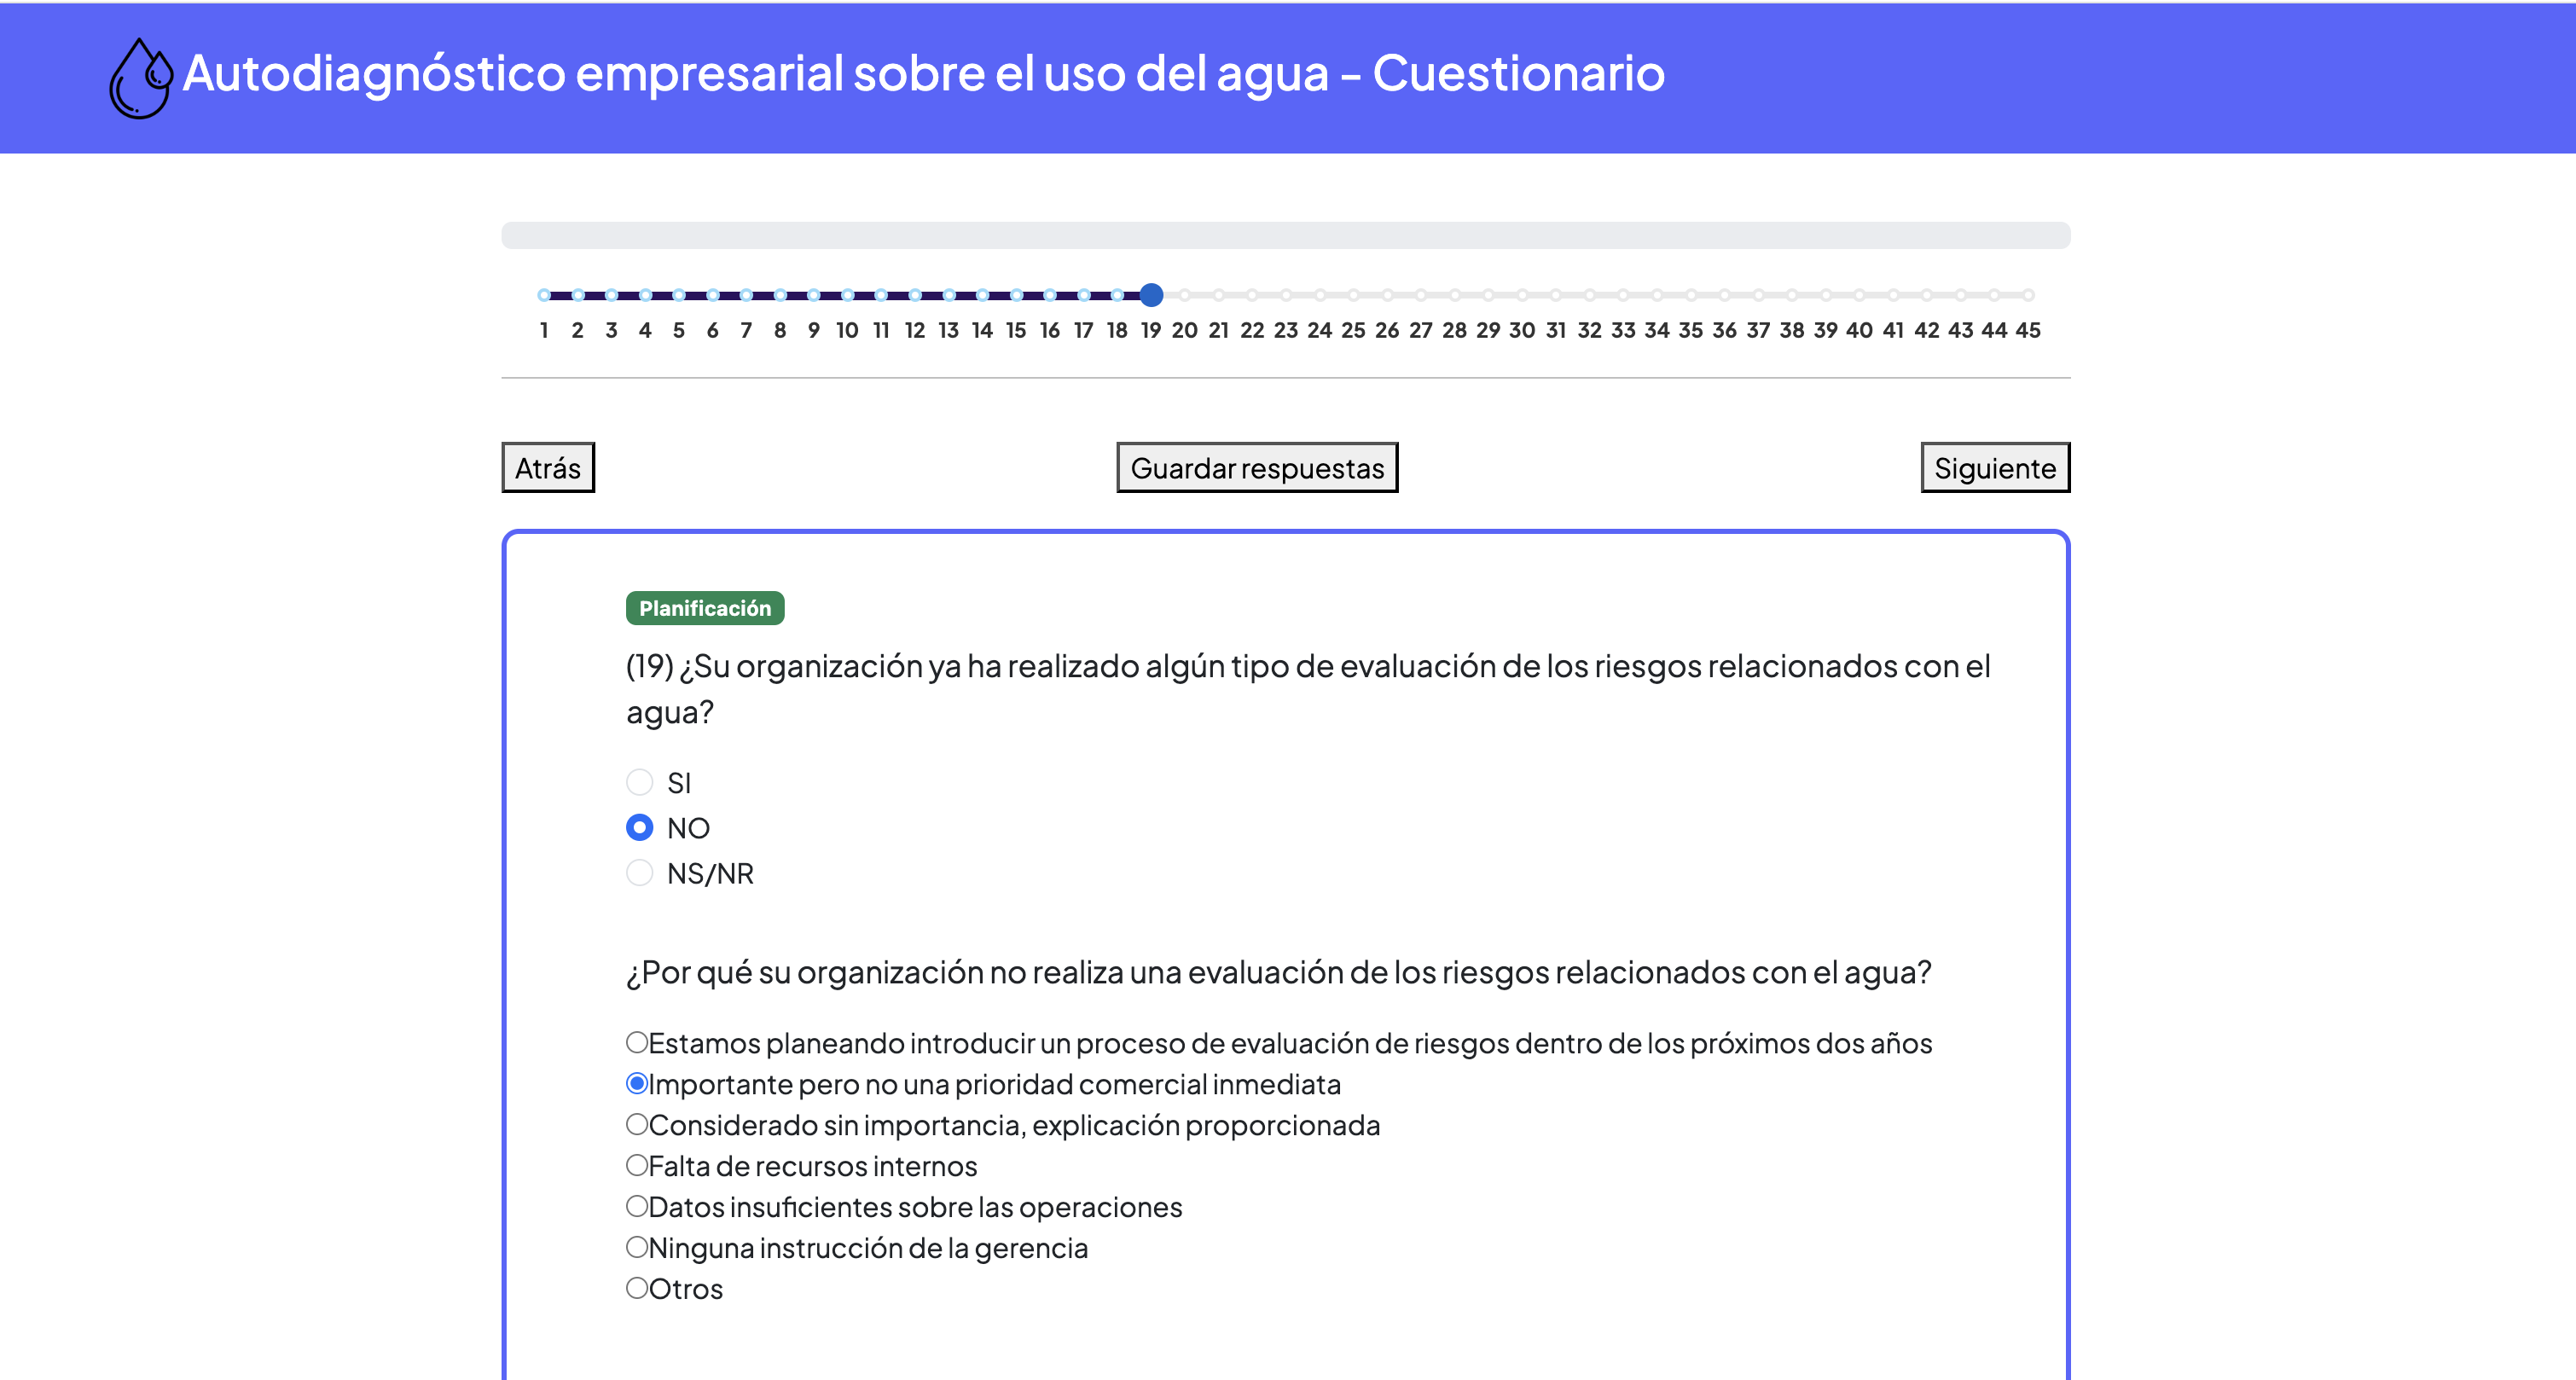
\includegraphics[scale=0.25]{images/99-aplicacion-web/3-cuestionario.png}
        \caption{Pantalla 'Cuestionaro' en la aplicación web}
\end{figure}

\begin{figure}[H]
        \centering
        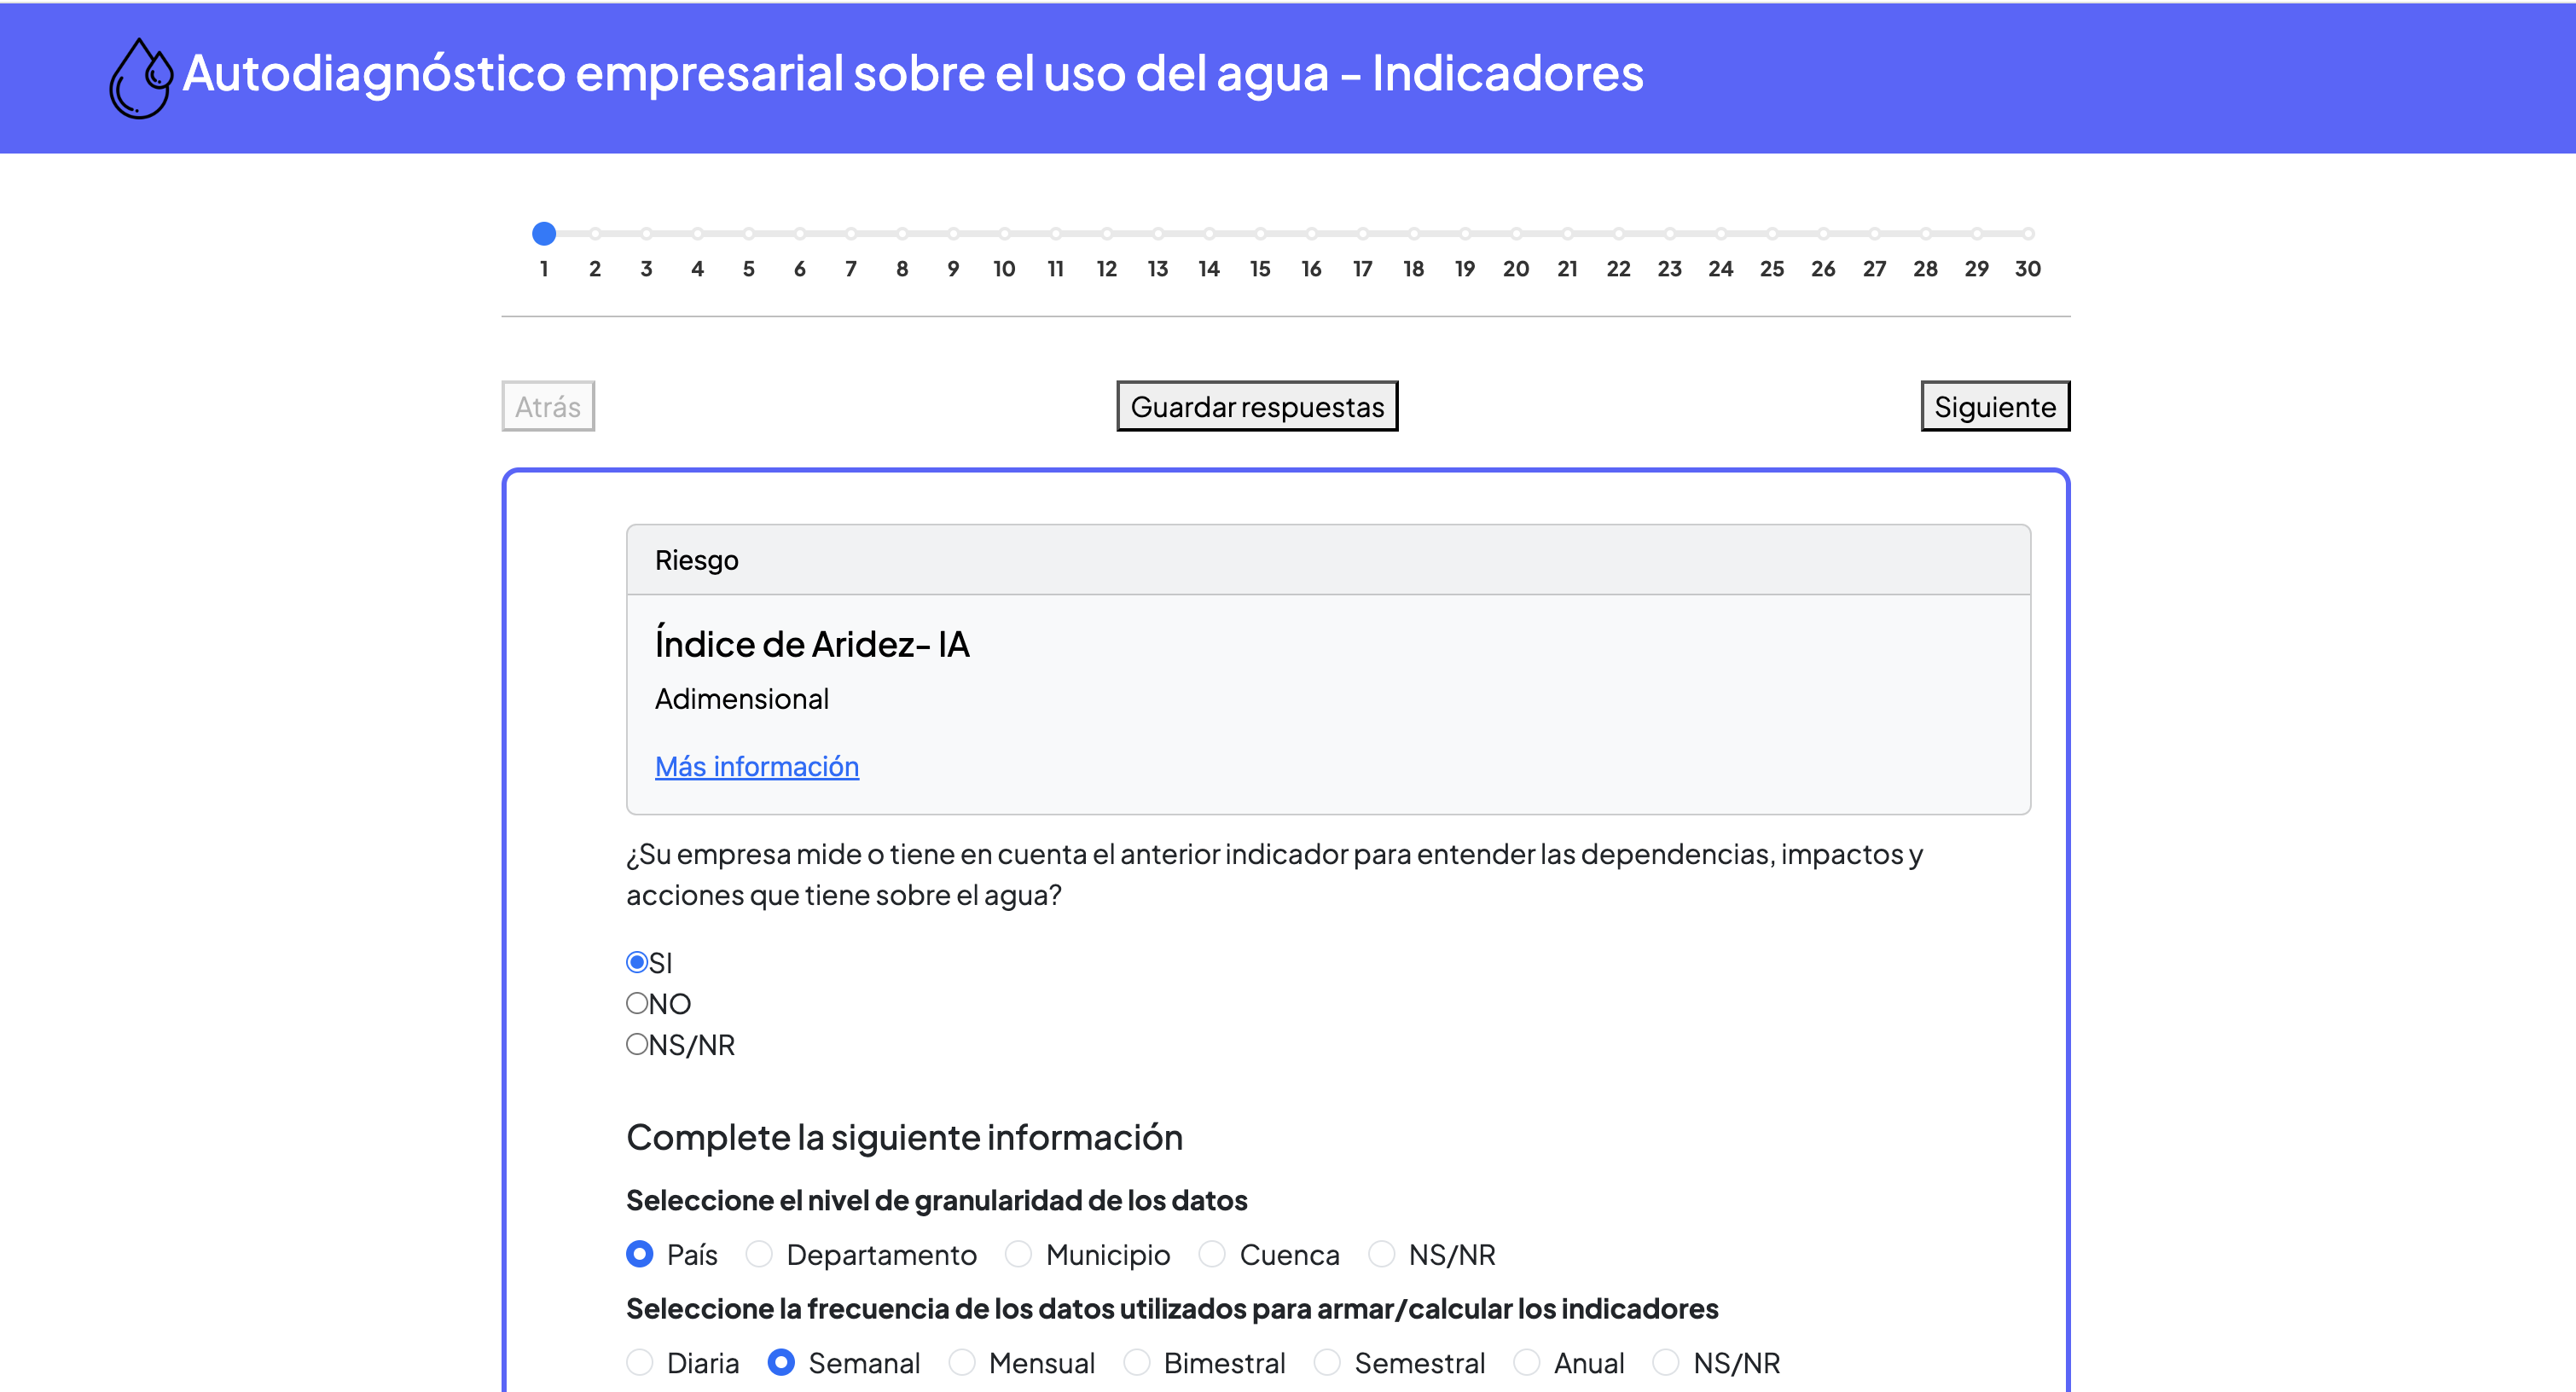
\includegraphics[scale=0.25]{images/99-aplicacion-web/4-indicadores.png}
        \caption{Pantalla 'Indicadores' en la aplicación web}
\end{figure}

\begin{figure}[H]
        \centering
        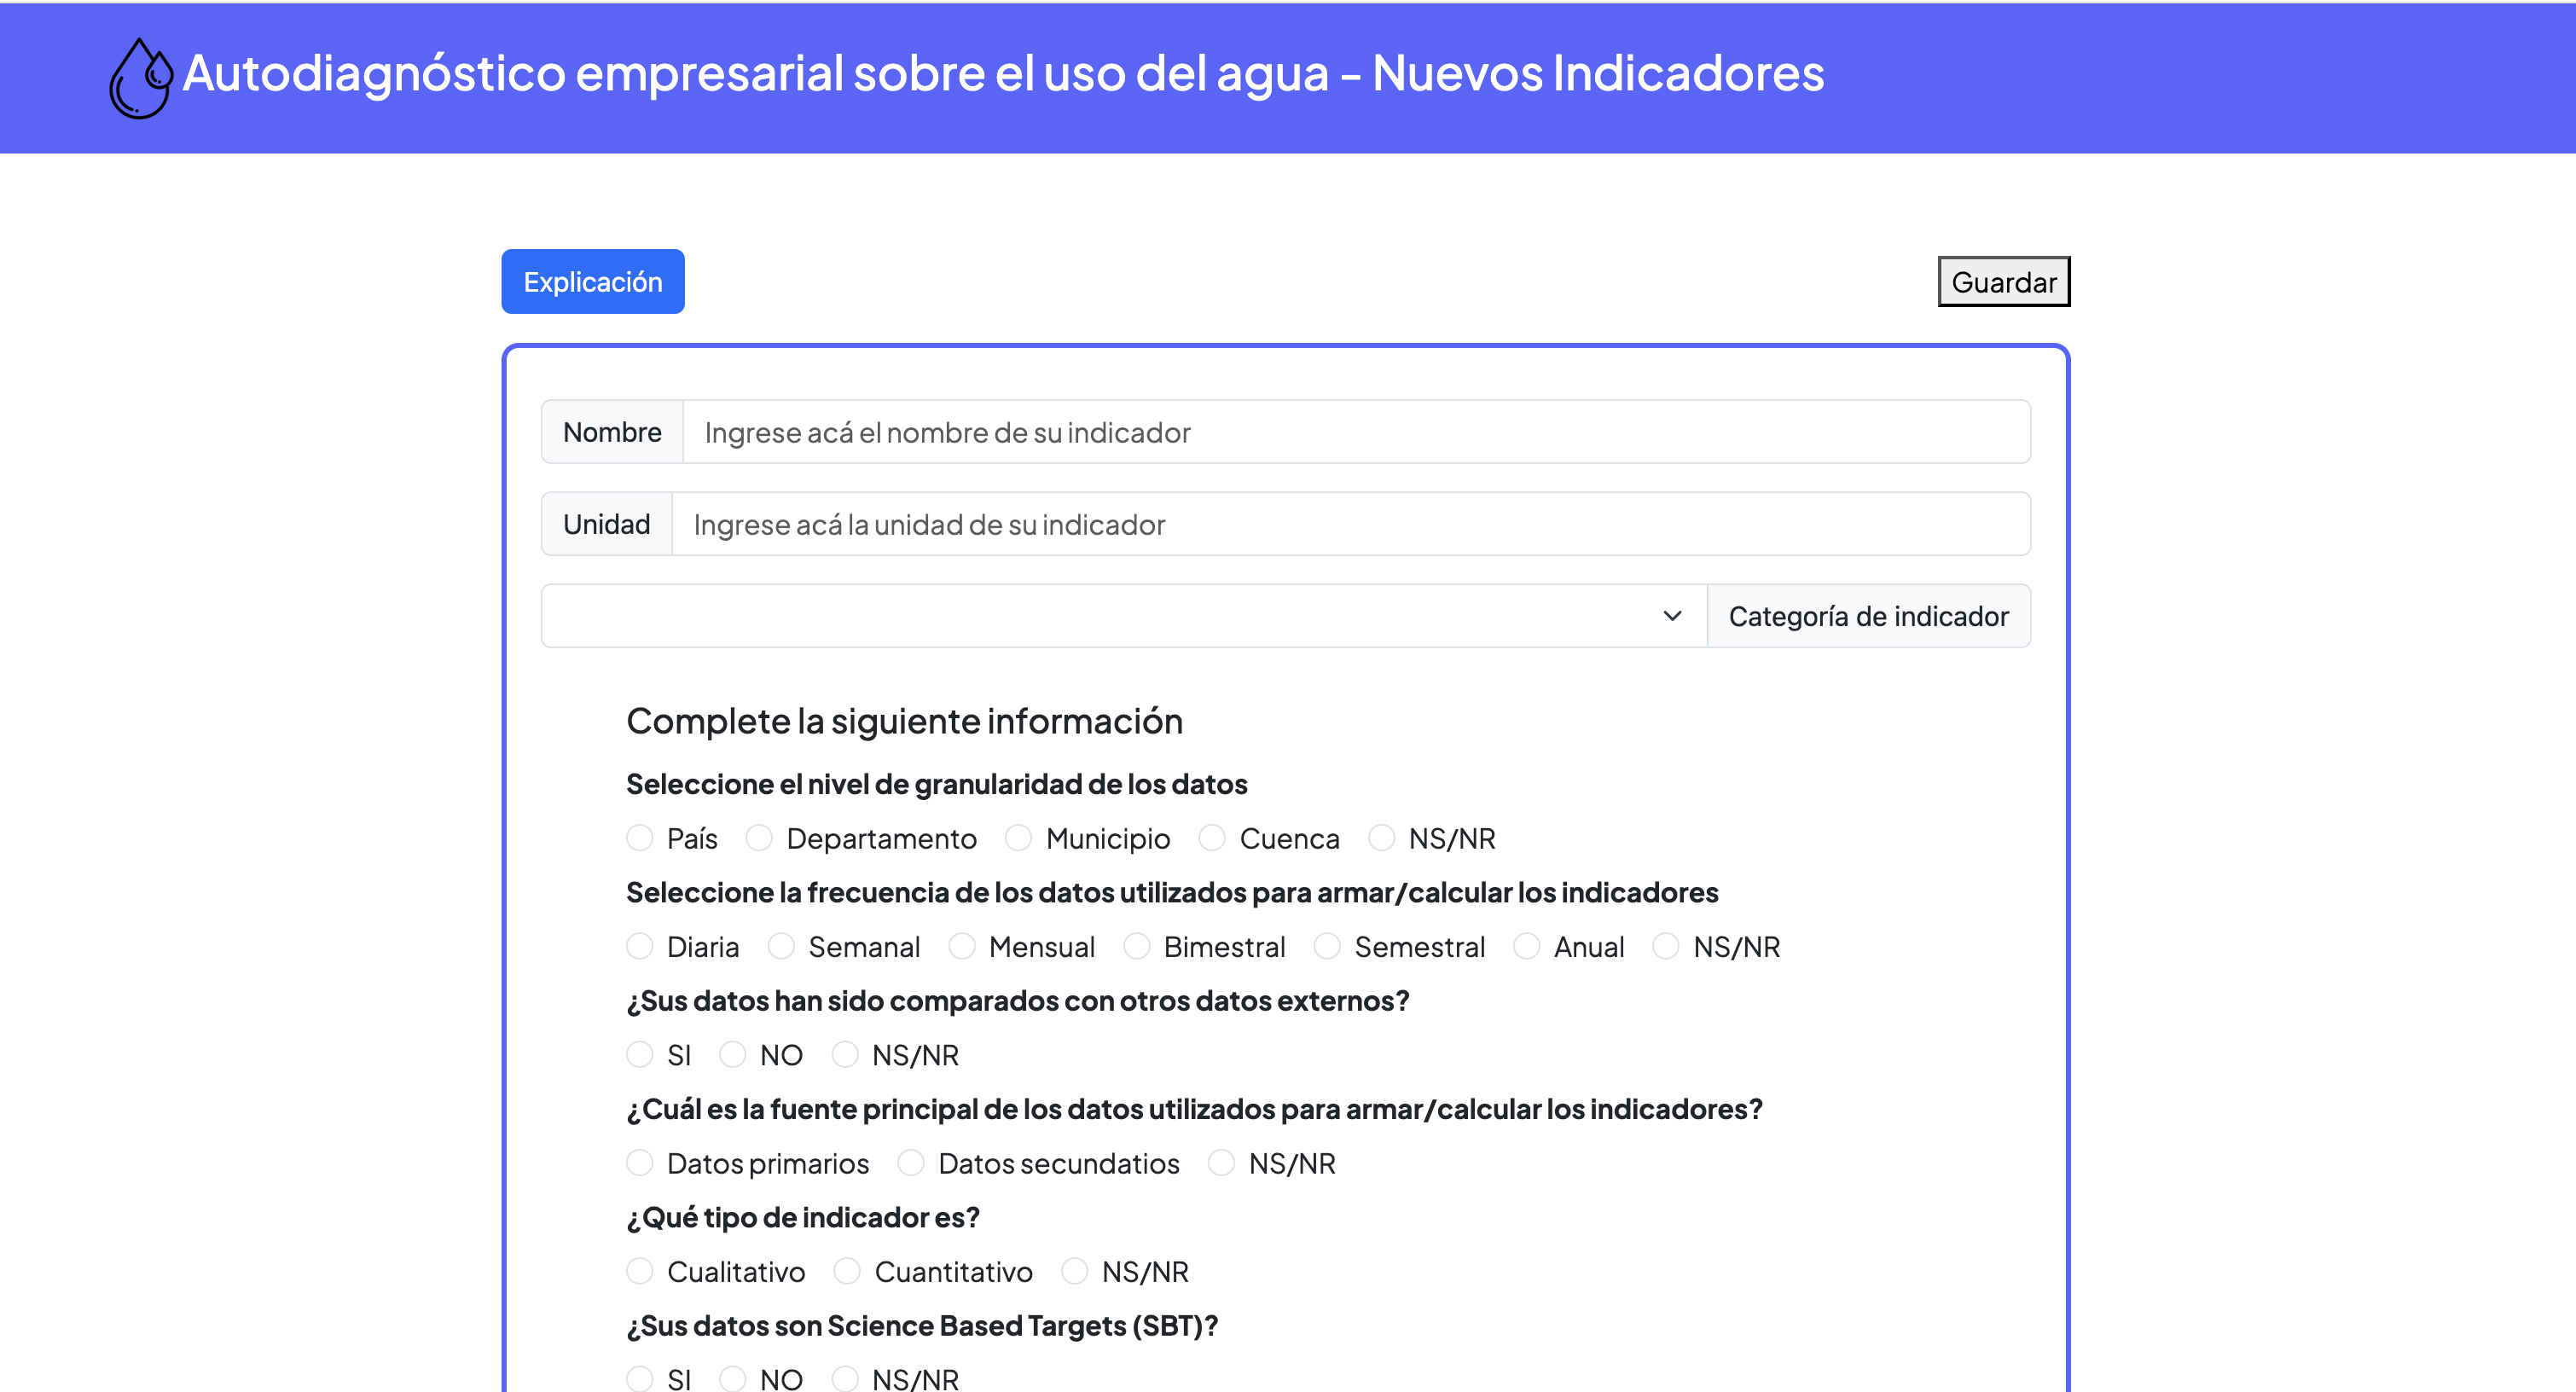
\includegraphics[scale=0.25]{images/99-aplicacion-web/5-nuevos-indicadores.png}
        \caption{Pantalla donde las empresas pueden agregar nuevos indicadores}
\end{figure}

\begin{figure}[H]
        \centering
        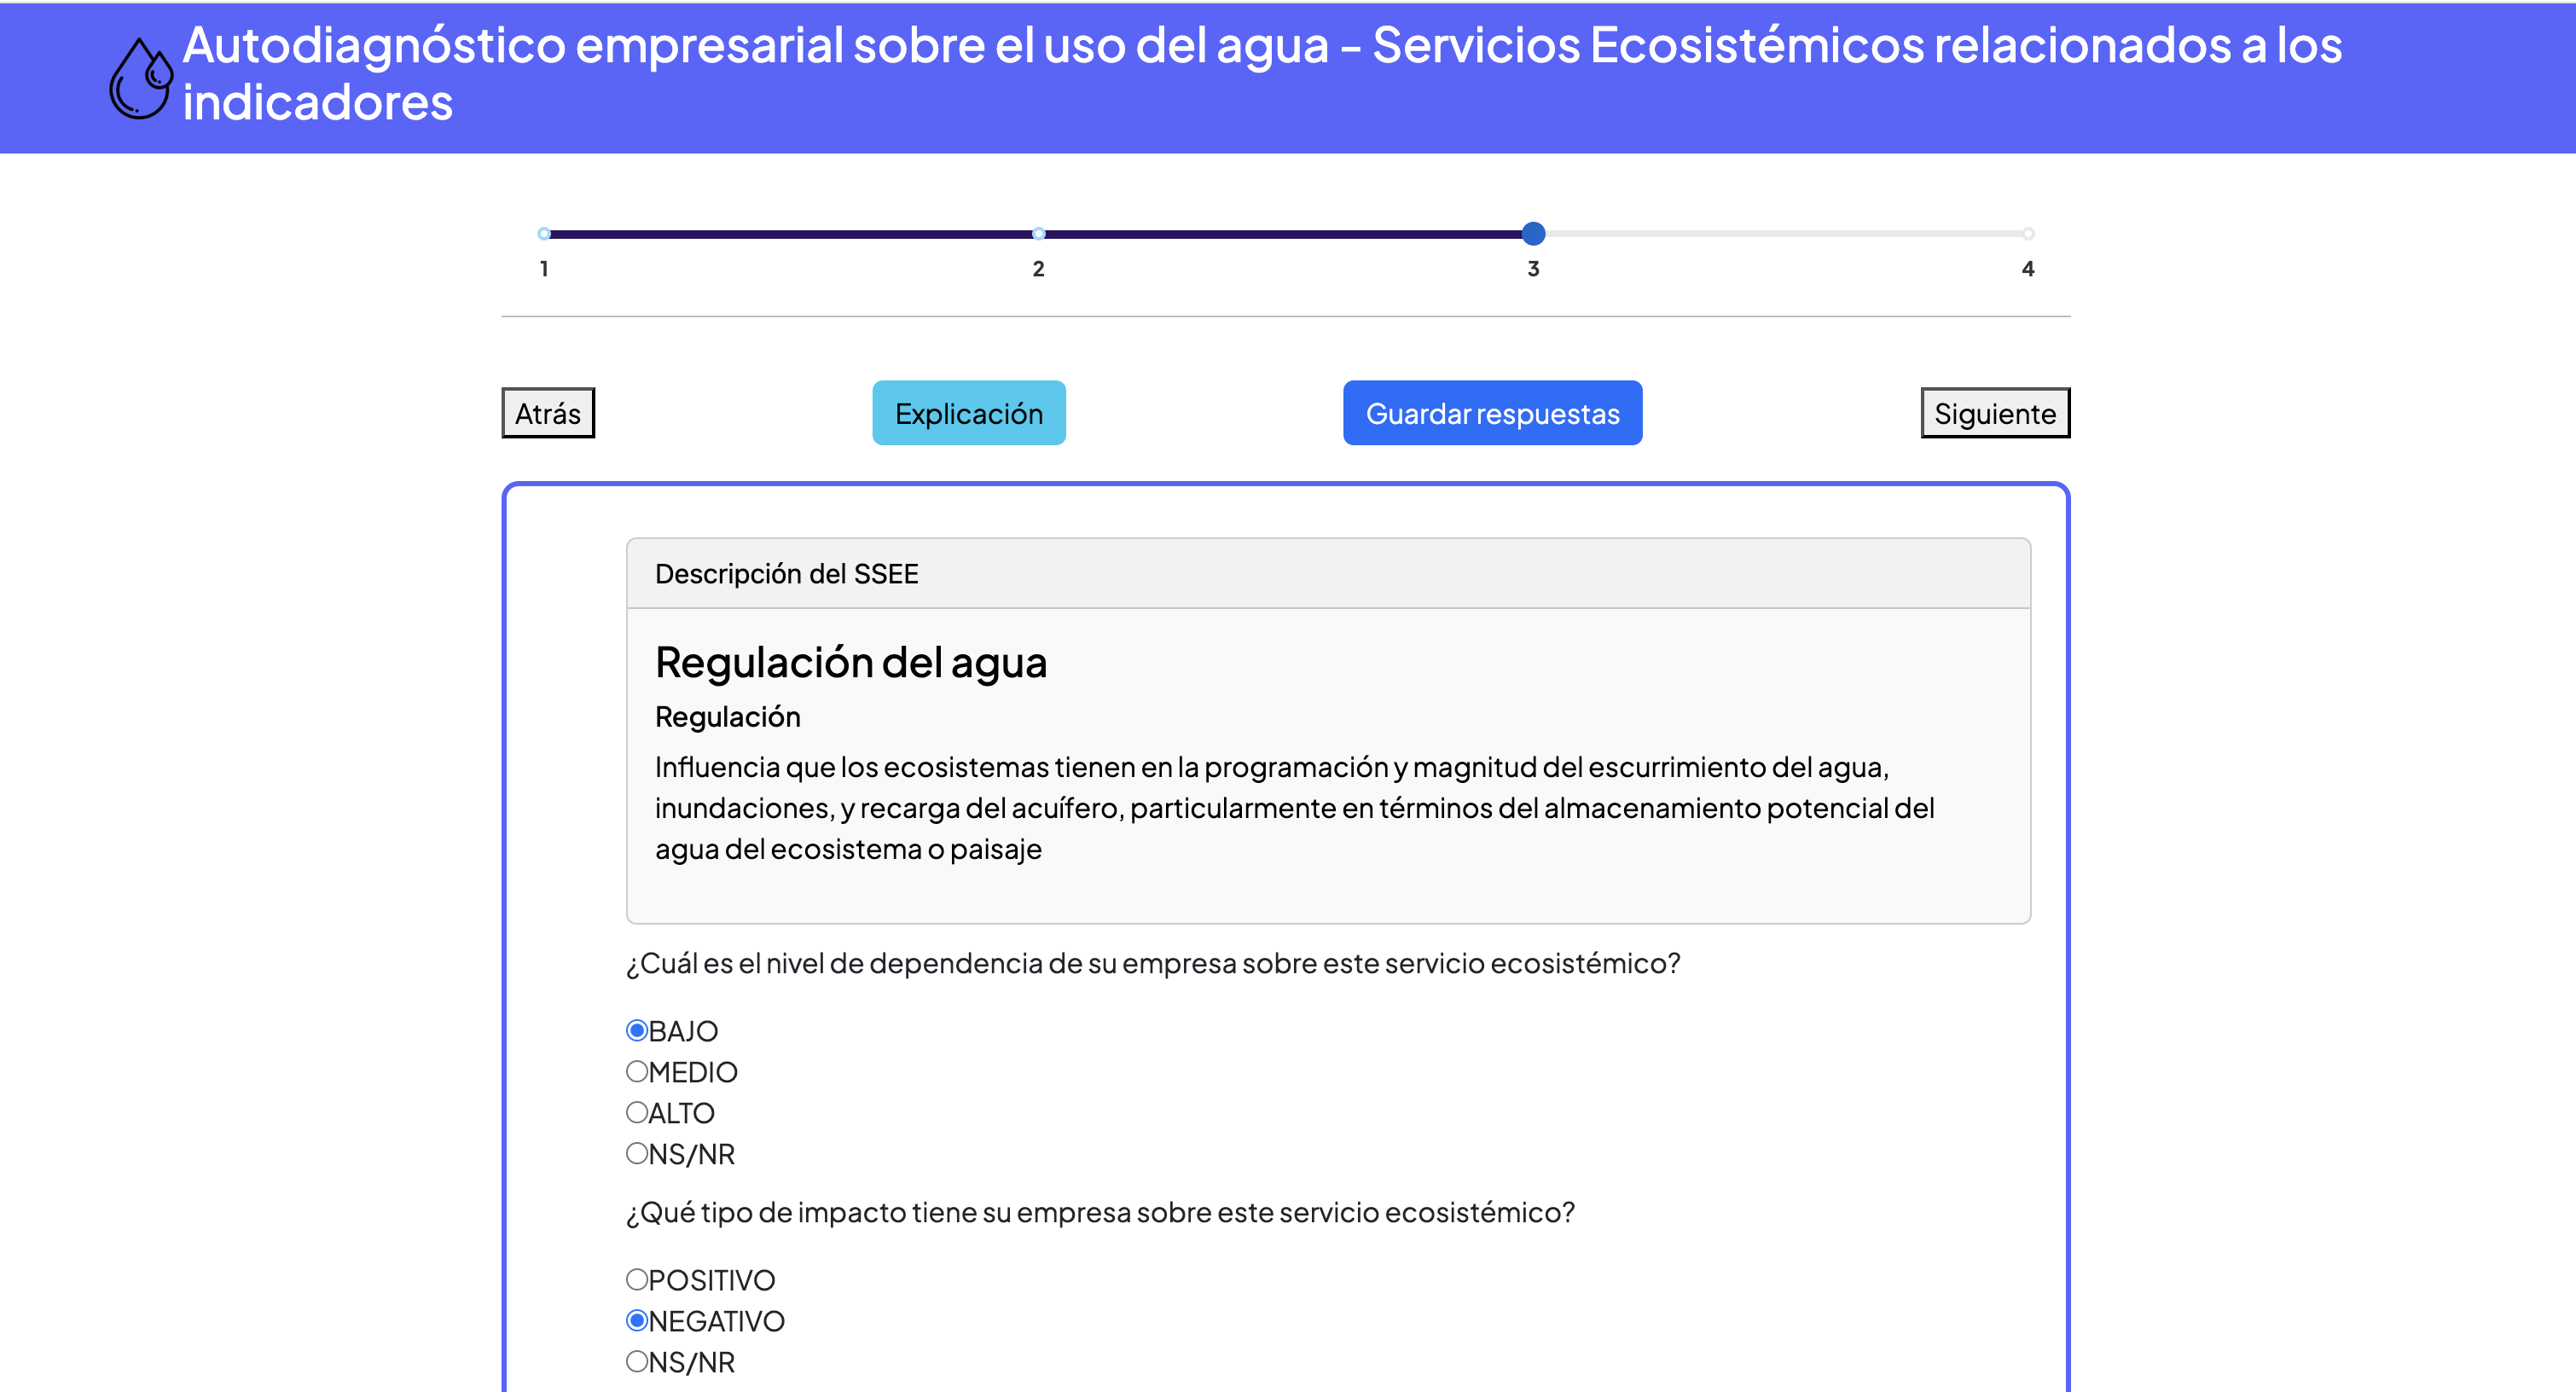
\includegraphics[scale=0.25]{images/99-aplicacion-web/6-ssee.png}
        \caption{Paso donde la empresa determina el nivel de dependencia y el tipo de impacto sobre un servicio ecosistémico}
\end{figure}

\begin{figure}[H]
        \centering
        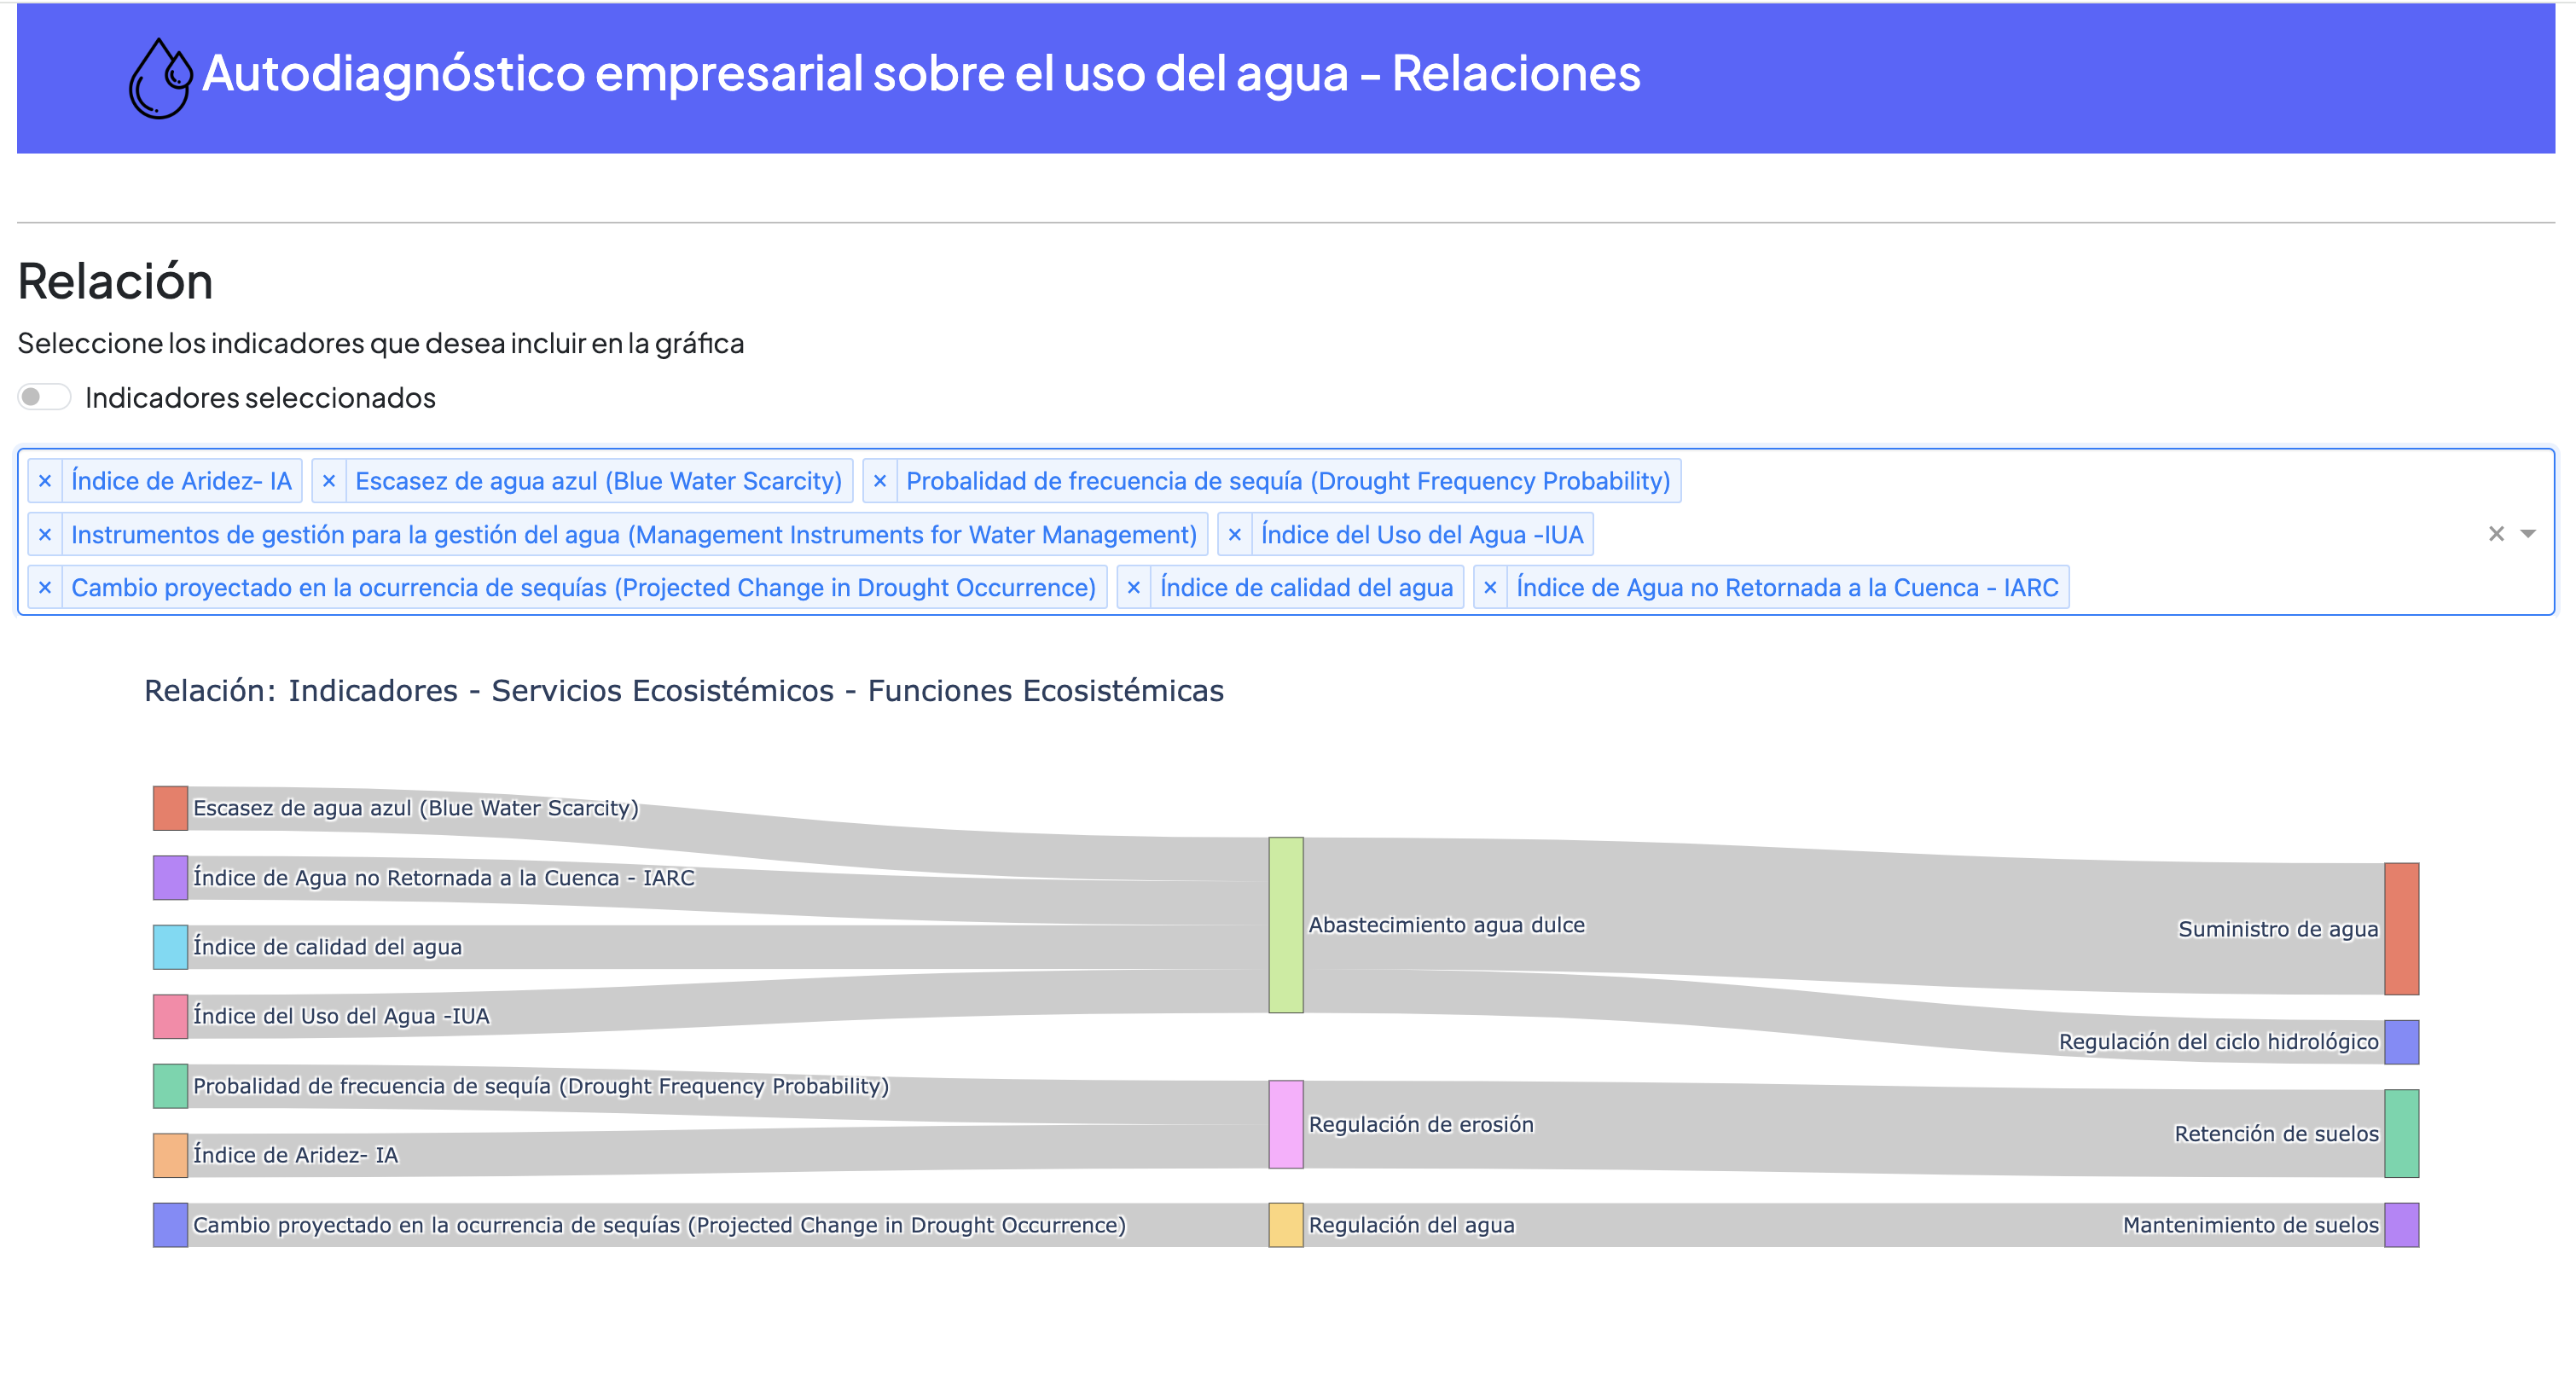
\includegraphics[scale=0.25]{images/99-aplicacion-web/7-relaciones.png}
        \caption{Pantalla donde se muestran las relaciones entre el negocio y los componentes del agua según los indicadores}
\end{figure}

\begin{figure}[H]
        \centering
        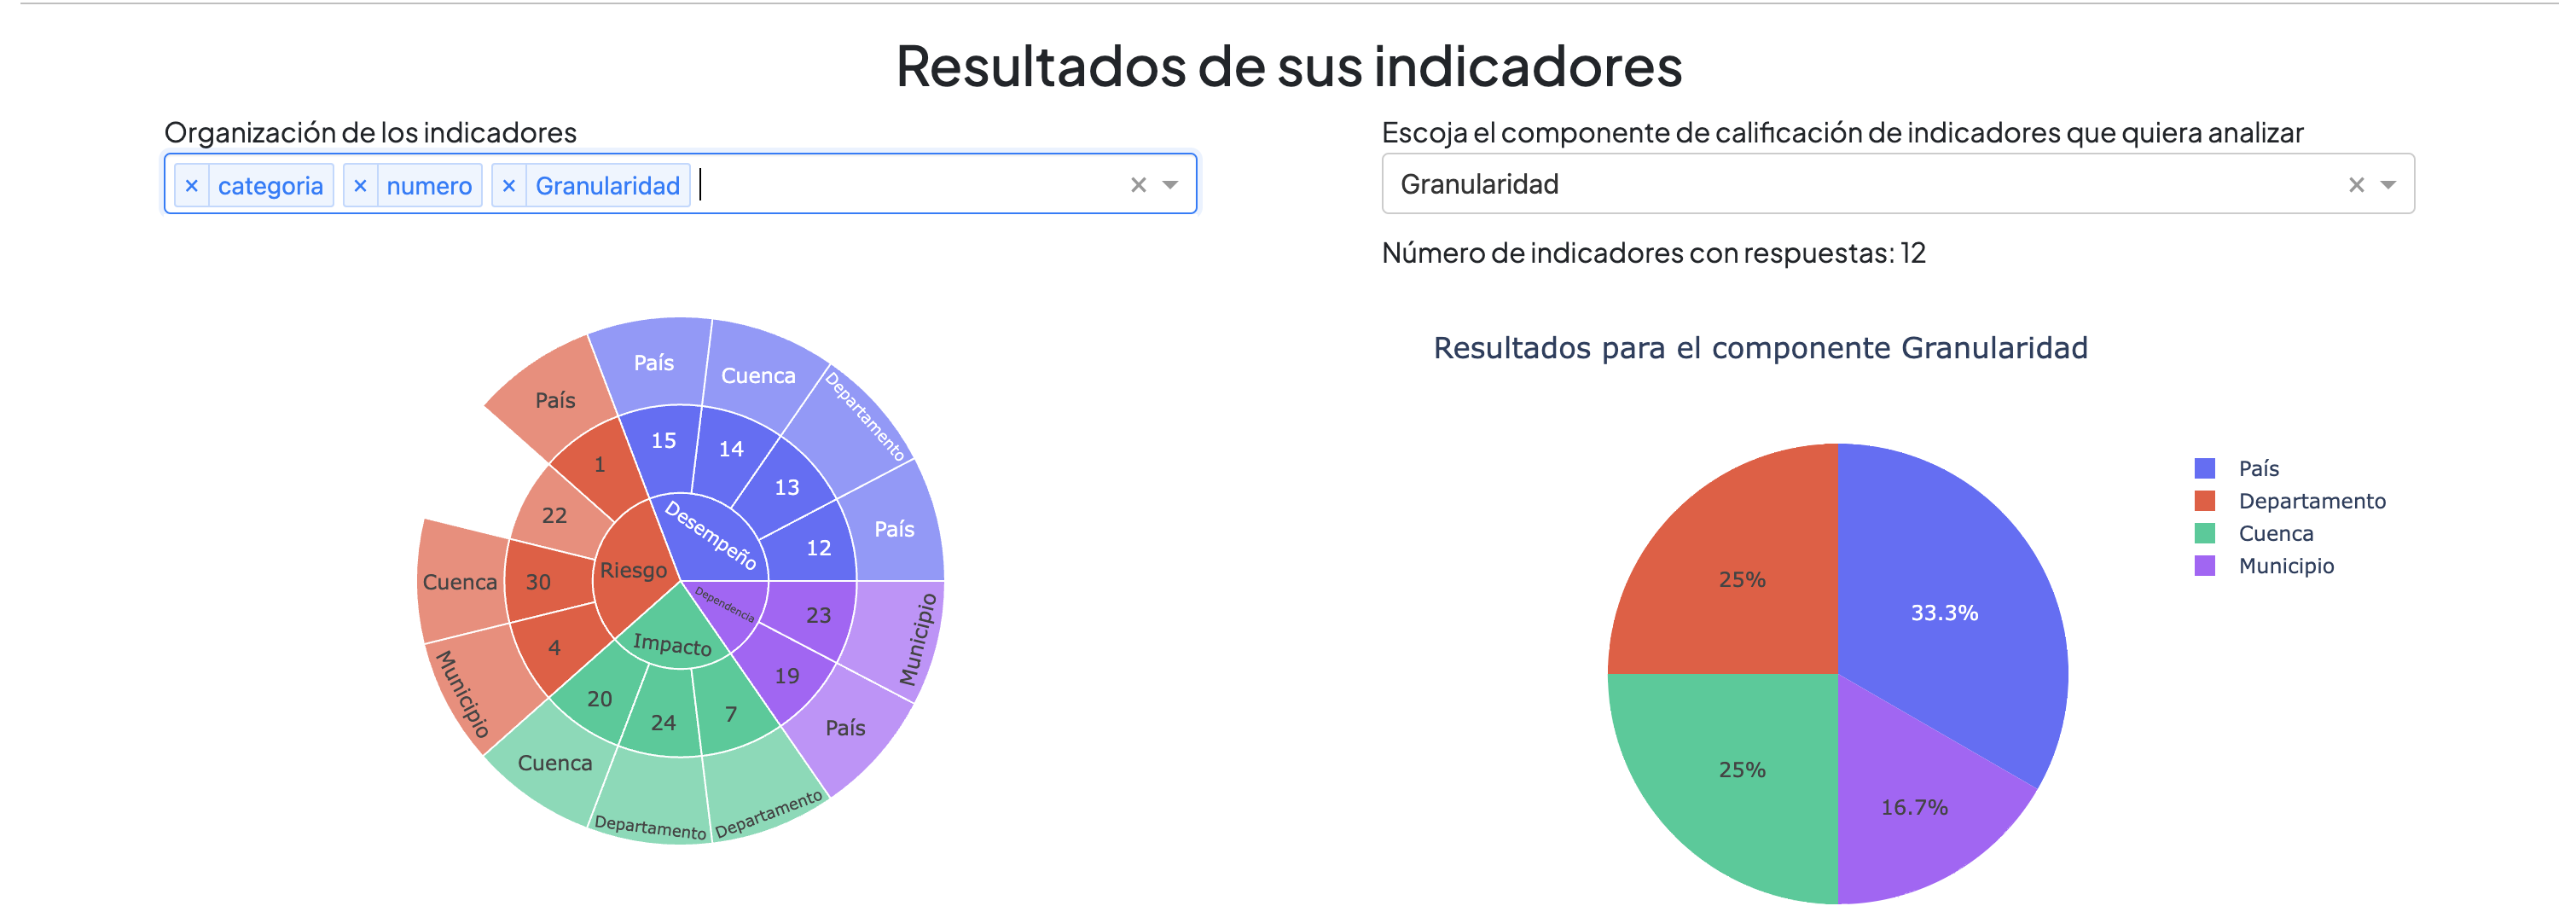
\includegraphics[scale=0.25]{images/99-aplicacion-web/10-respuestas-indicadores.png}
        \caption{Estadísitcas descriptivas de los indicadores seleccionados por la empresa}
\end{figure}

\section{Validación}
\subsection{Formulario}\label{apx:formulario}
\begin{longtable}{p{2.5cm}|p{8cm}|p{5cm}}
    \textbf{Atributo} & \textbf{Pregunta} & \textbf{Opciones}\\
    \hline\hline
    Funcionalidad & ¿Las funciones disponibles en la aplicación cubren todas sus necesidades para evaluar las dependencias e impactos de su empresa sobre el agua? & Sí, No \\
\hline
Funcionalidad & ¿Encontró alguna función que no estuviera disponible y que considere esencial? & Sí, No \\
\hline
Confiabilidad & ¿La aplicación se ha comportado de manera consistente y sin errores durante su uso? & Siempre, A veces, Raramente, Nunca \\
\hline
Confiabilidad & ¿Ha experimentado pérdida de datos o información incorrecta al usar la aplicación? & Sí, No \\
\hline
Usabilidad & ¿Considera que la interfaz de usuario es intuitiva y fácil de usar? & Totalmente de acuerdo, De acuerdo, Neutral, En desacuerdo, Totalmente en desacuerdo \\
\hline
Usabilidad & ¿Cuánto tiempo le tomó familiarizarse con el uso de la aplicación? & Menos de 30 minutos, Entre 30 minutos y 1 hora, Más de 1 hora \\
\hline
Usabilidad & ¿Cuánto tiempo le tomó terminar el cuestionario de la aplicación? & Menos de 30 minutos, Entre 30 minutos y 1 hora, Más de 1 hora \\
\hline
Rendimiento & ¿La velocidad de carga y respuesta de la aplicación es satisfactoria? & Muy satisfactoria, Satisfactoria, Neutral, Insatisfactoria, Muy insatisfactoria \\
\hline
Rendimiento & ¿Ha experimentado tiempos de espera prolongados o bloqueos al usar la aplicación? & Sí, No \\
\hline
Contexto & ¿La aplicación le proporciona suficiente información para entender su nivel de madurez en relación a las dependencias e impactos sobre el agua? & Totalmente de acuerdo, De acuerdo, Neutral, En desacuerdo, Totalmente en desacuerdo \\
\hline
Contexto & ¿Las preguntas del cuestionario inicial son claras y relevantes para su contexto organizacional? & Totalmente de acuerdo, De acuerdo, Neutral, En desacuerdo, Totalmente en desacuerdo \\
\hline
Practicidad & ¿Considera que la aplicación es práctica para el uso en su empresa? & Totalmente de acuerdo, De acuerdo, Neutral, En desacuerdo, Totalmente en desacuerdo \\
\hline
Practicidad & ¿Recomendaría esta aplicación a otras empresas para evaluar sus impactos y dependencias sobre el agua? & Sí, No \\
\hline
Visualizaciones Finales & ¿Las visualizaciones proporcionadas al final del proceso son claras y fáciles de entender? & Totalmente de acuerdo, De acuerdo, Neutral, En desacuerdo, Totalmente en desacuerdo \\
\hline
Visualizaciones Finales & ¿Las gráficas descriptivas y los resultados por dimensión le resultaron útiles para su análisis? & Totalmente de acuerdo, De acuerdo, Neutral, En desacuerdo, Totalmente en desacuerdo \\
\hline
Utilidad & ¿La aplicación le ha ayudado a identificar nuevas áreas de mejora en la gestión del agua en su empresa? & Totalmente de acuerdo, De acuerdo, Neutral, En desacuerdo, Totalmente en desacuerdo \\
\hline
Utilidad & ¿Considera que la aplicación cumplió con los objetivos establecidos (determinar nivel de madurez, entender mejor dimensión, exponer indicadores)? & Totalmente de acuerdo, De acuerdo, Neutral, En desacuerdo, Totalmente en desacuerdo \\
\hline
\caption{Preguntas realizadas en el formulario de validación}
\label{tab:formulari-validacion}
\end{longtable}
    



\clearpage


% Referencias

\printbibliography[
heading=bibintoc
]

\end{document}

\endinput
